% !TeX TS-program = xelatex
\documentclass[12pt]{article}
%\usepackage[utf8]{inputenc}
\usepackage{indentfirst}
\usepackage{float}
\usepackage{array}
\usepackage{comment}
\usepackage{url}
\urlstyle{tt}
\usepackage{enumitem, amsmath, amssymb, amsfonts, latexsym, mathrsfs}
\usepackage{graphicx}
\usepackage{subfig}
\usepackage{multicol}
\usepackage{booktabs}
\usepackage{ragged2e}
\usepackage{svg}
\usepackage{xcolor}
\usepackage{tabularray}
\usepackage{listings}
\usepackage{atkinson} %% Option 'sfdefault' if the base
%% font of the document is to be sans serif.
% \usepackage[T1]{fontenc}


\usepackage{fontspec}
\setmainfont{Atkinson Hyperlegible}
\renewcommand{\familydefault}{\sfdefault}

%\setmainfont{Geist}[
%  Path=./fonts/Geist/,
%  Extension=.otf,
%  UprightFont=*-Regular,
%  BoldFont=*-Bold
%]

\setmonofont{GeistMono}[
  Path=./fonts/GeistMono/,
  Extension=.otf,
  UprightFont=*-Regular,
  BoldFont=*-Bold
]

\usepackage[spanish]{babel}

\usepackage[backend=biber]{biblatex}
\bibliography{referencias}
\usepackage{csquotes}
%New colors defined belowd
\usepackage{}
\definecolor{codegreen}{rgb}{0,0.6,0}
\definecolor{codegray}{rgb}{0.5,0.5,0.5}
\definecolor{codepurple}{rgb}{0.58,0,0.82}
\definecolor{backcolour}{rgb}{0.95,0.95,0.92}
\lstdefinestyle{mystyle}{
  backgroundcolor=\color{backcolour},   commentstyle=\color{codegreen},
  keywordstyle=\color{magenta},
  numberstyle=\tiny\color{codegray},
  stringstyle=\color{codepurple},
  basicstyle=\ttfamily\footnotesize,
  breakatwhitespace=false,
  breaklines=true,
  captionpos=b,
  keepspaces=true,
  numbers=left,
  numbersep=5pt,
  showspaces=false,
  showstringspaces=false,
  showtabs=false,
  tabsize=2
}
%"mystyle" code listing set
\lstset{style=mystyle}
%\lstset{basicstyle=\ttfamily\footnotesize,breaklines=true}

\usepackage{notoccite}

\usepackage{multicol}
\setlength{\columnseprule}{1pt}
\def\columnseprulecolor{\color{black}}





\date{}
% Comand para keywords
\providecommand{\keywords}[1]
{
  \small
  \textbf{\textit{Keywords---}} #1
}

% Tipografía
%\usepackage{helvet}
%\renewcommand{\familydefault}{\sfdefault}
%\usepackage[sfdefault]{Chivo}
%\usepackage{comment}


\urlstyle{same}
% \tolerance=9999
% \emergencystretch=10pt
\hyphenpenalty=10000
\sloppy
% \exhyphenpenalty=100

\renewcommand{\figurename}{\textbf{Figura.}}
\renewcommand\spanishtablename{Tabla.}

% Interlineado
\usepackage{setspace}
\spacing{1.15}

% Márgenes
\usepackage[a4paper]{geometry}
\geometry{top=2.5cm, bottom=2.5cm, left=2cm, right=2cm}

% Número de página
\usepackage{fancyhdr}
\pagestyle{fancy}
\rhead[]{}
\lhead[]{}
\renewcommand{\headrulewidth}{0pt}
\rfoot[]{\thepage}
\cfoot[]{}

\usepackage[breaklinks]{hyperref}
% Setup de hiperenlaces
\hypersetup{
    colorlinks=true,
    linkcolor=blue,
    filecolor=magenta,
    urlcolor=cyan,
    pdftitle={Apuntes de Consolas y Videojuegos},
    pdfpagemode=FullScreen,
    citecolor = green
    }
\usepackage[norule]{footmisc}

%_____________________________________________________________________________
%_____________________________________________________________________________
%_____________________________________________________________________________
%_____________________________________________________________________________
\hbadness=50000
\usepackage{microtype}
\begin{document}
\nocite{atkinson}
\nocite{circuitverse}
\nocite{chatgpt}
\nocite{duke}
\nocite{texstudio}
% PORTADA
\begin{titlepage}
        \begin{center}


        \hrule
        \vspace{1cm}
        %{\bfseries\Large UNIVERSIDAT JAUME I \par}
        \vspace{1cm}
        {\bfseries\huge Apuntes de Consolas y Dispositivos de Videojuegos \par}
        \vspace{2cm}

        \begin{figure}[H]
            \centering
            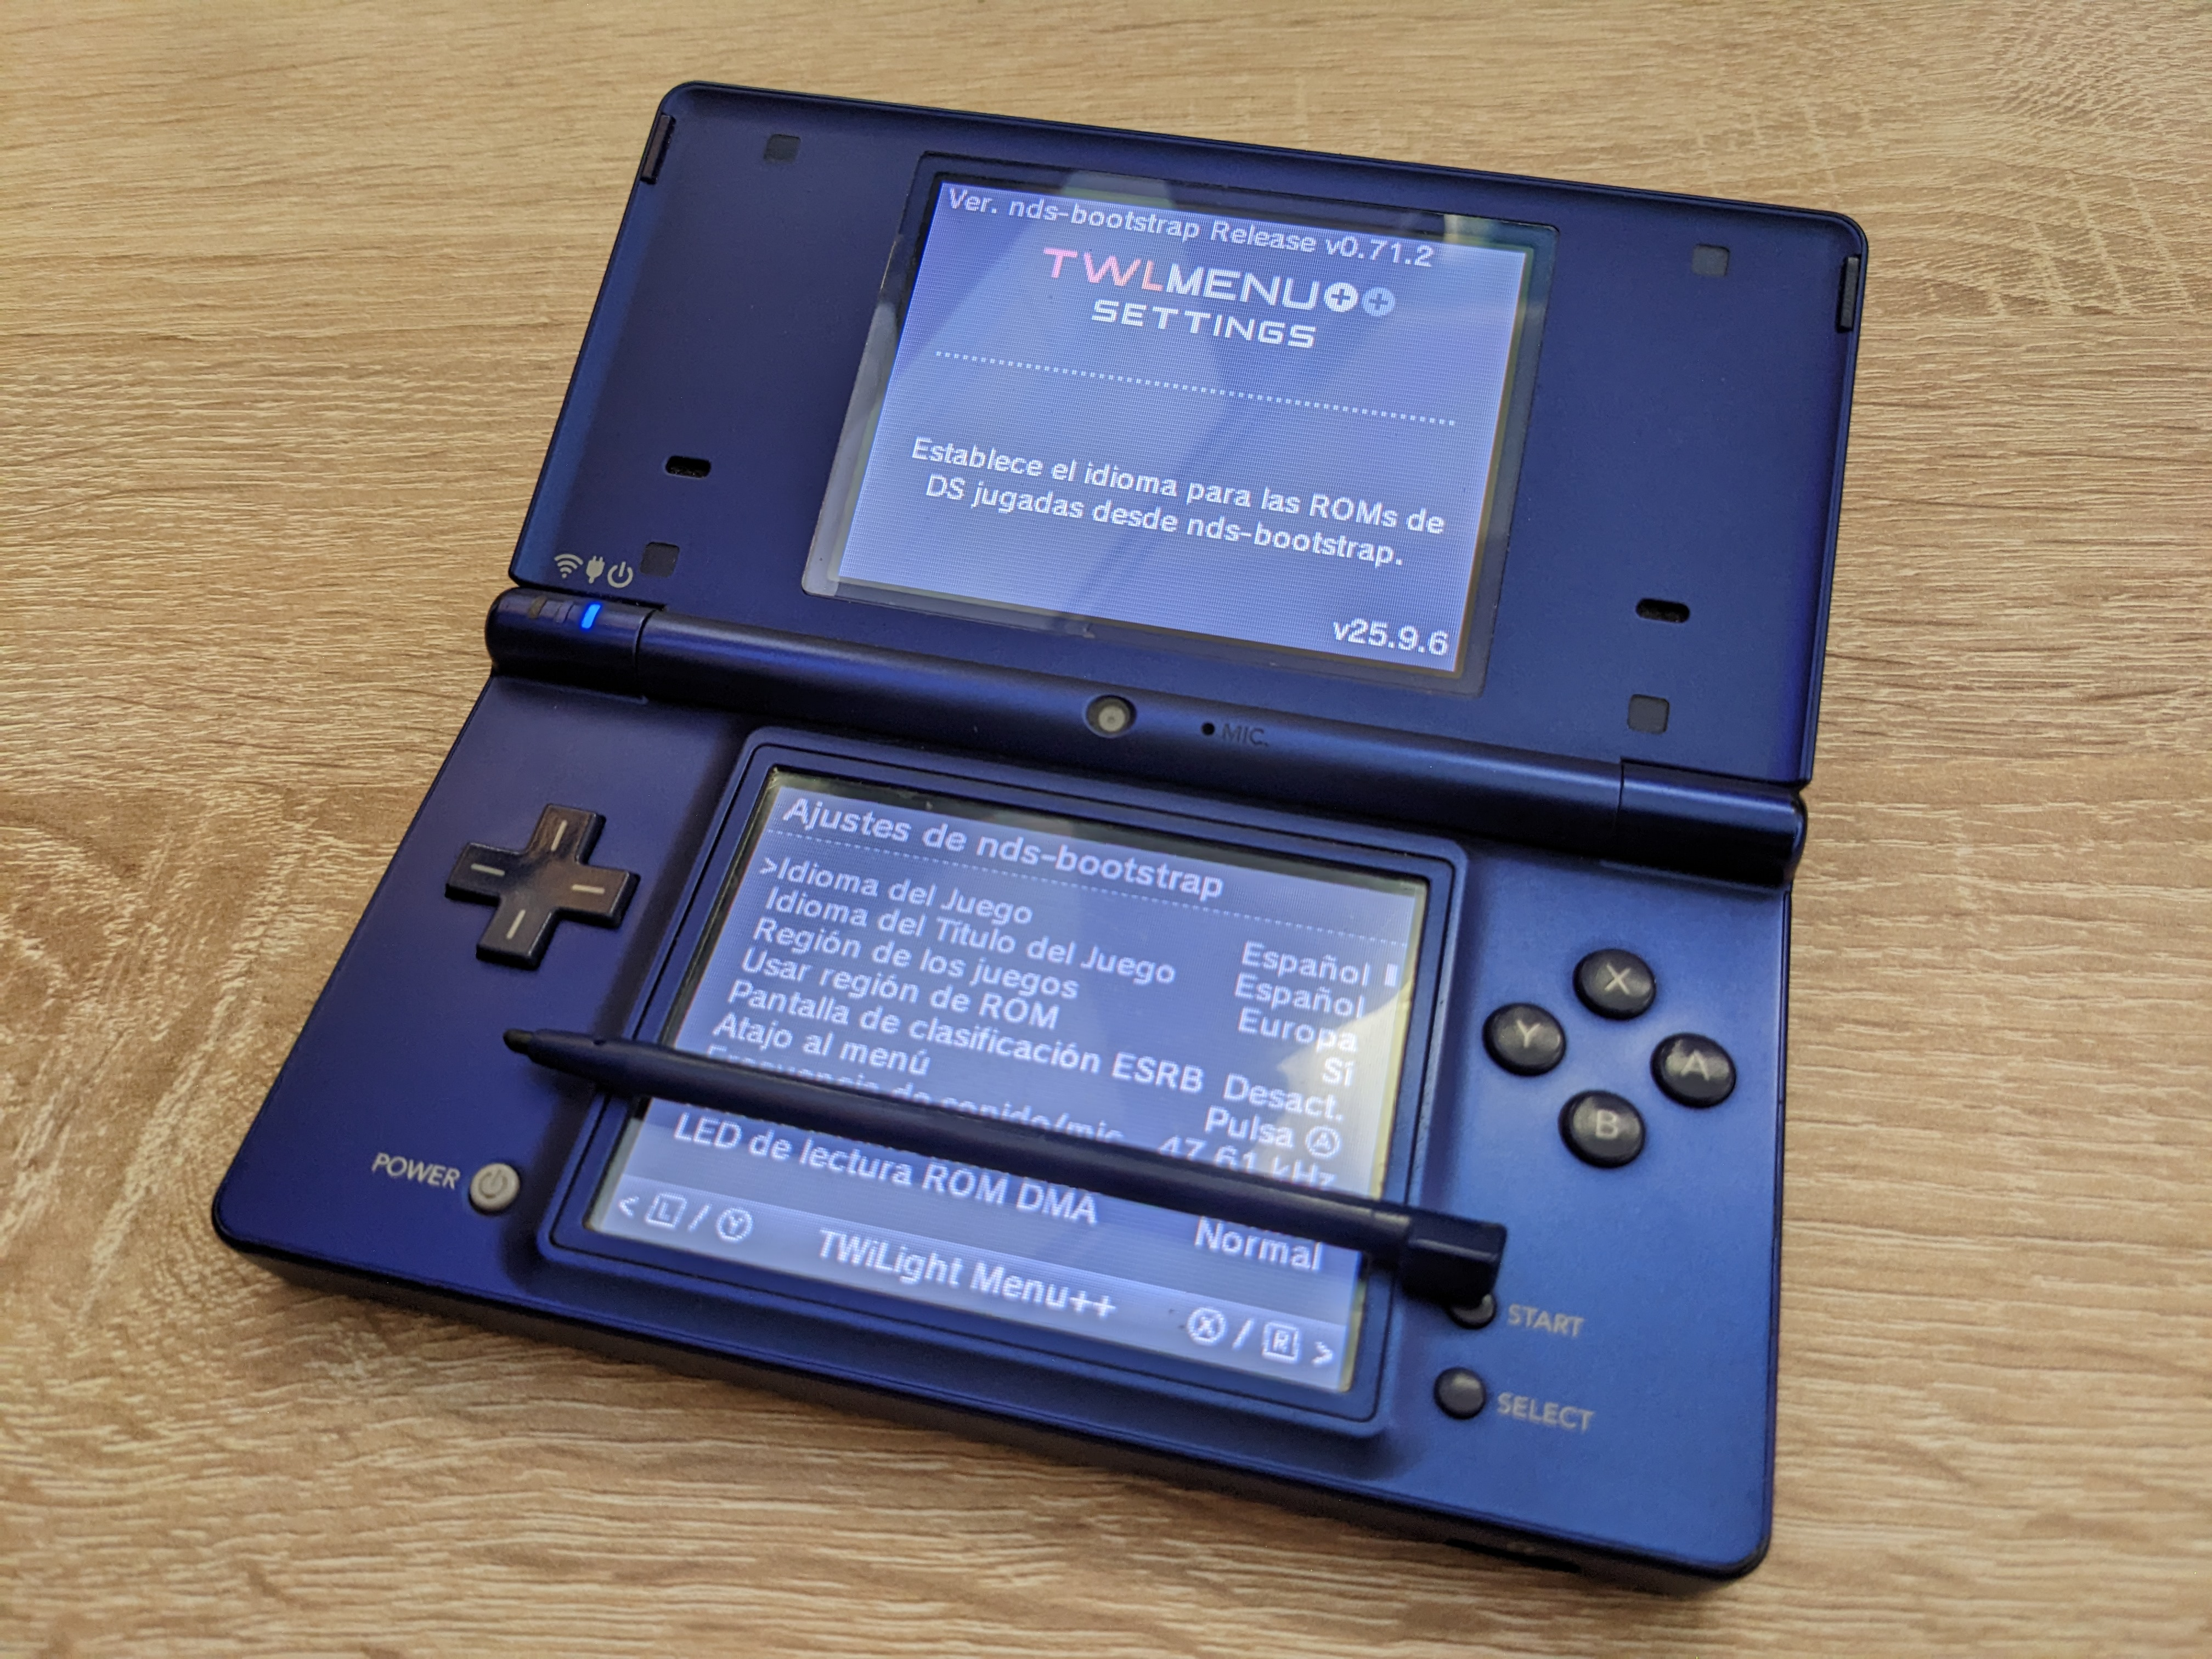
\includegraphics[width=\textwidth]{dsi.jpg}
            \caption*{\footnotesize{\textit{Nintendo DSi con Homebrew y emulador de NDS}}}
            \label{fig:dsi}
        \end{figure}

        {\large
        Jesús Jiménez Montero \\
        \par}
        \vspace{1cm}
        \hrule
        \vspace{1cm}

        {\large
        \textit{Versión 5: Registros y RAM\\
        \today}
        \par}
        \end{center}
\end{titlepage}

% ÍNDICE
%\renewcommand{\tableofcontents}{Indice general}
\newpage
\renewcommand{\contentsname}{Tabla de contenidos}
\setcounter{secnumdepth}{5}
\tableofcontents
\setcounter{tocdepth}{4}

\newpage
%-----------------------------------------------------------------
%-----------------------------------------------------------------
% Tabla de figuras
\newpage
\renewcommand{\listfigurename}{Lista de figuras}
\thispagestyle{empty}
\listoffigures
\newpage

\renewcommand{\listtablename}{Lista de tablas}
\listoftables
\newpage

%-----------------------------------------------------------------
\begin{comment}
	\section{Circuito}
	\subsection{Tabla de verdad y explicación del circuito}

	\subsection{Esquema del circuito exterior y exterior}

	\subsection{Implementación HDL}

		\subsubsection{Archivo .HDL}
			\begin{lstlisting}

			\end{lstlisting}
		\subsubsection{Archivo .TST}
			\begin{lstlisting}

			\end{lstlisting}
		\subsubsection{Archivo .CMP}
			\begin{lstlisting}

			\end{lstlisting}

\newpage
\end{comment}
%-----------------------------------------------------------------
%%%%%%%%%%%%%%%%%%%%%%%%%%%%%%%%%%%%%%%%%%%%%%%%%%%%%%%%%%%%%%%%%%%%%%%%%%
%%%%%%%%%%%%%%%%%%%%%%%%%%%%%%%%%%%%%%%%%%%%%%%%%%%%%%%%%%%%%%%%%%%%%%%%%%
\begin{comment}

\part{El álgebra de Boole}
\section{El álgebra de Boole}

\subsection{Definición del algebra de Boole \cite{floyd_fundamentos_2006} \cite{logic_gate} \cite{puerta_logica}}
El álgebra de Boole es basicamente las matématicas que se usan en computación, necesarias para analizar los circuitos lógicos.

Para realizar esta álgebra se usan varios términos: variable, que referencia a una magnitud que se resume en los valores 0 y 1 y los complementos, que son los inversos de una variable, representados con una barra ($A \rightarrow \overline{A}$).

Las puertas lógicas son circuitos que realizan operaciones lógicas determinadas:

\subsubsection{\textbf{Puerta lógica NOT}}

Negación booleana, $A$ pasa a ser no $A$, es decir, $\overline{A}$.

\begin{multicols}{2}

	\begin{table}[H]
		\centering
		\begin{tabular}{|c|c|}
			$A$ & $\overline{A}$ \\
			\hline
			0 & 1 \\
			1 & 0
		\end{tabular}
		\caption{Tabla de verdad de NOT}
		\label{tab:not}
	\end{table}

	\columnbreak
	\newpage
	\begin{figure}[H]
		\centering
		\includesvg{CIRCUITOS/NOT_ANSI_Labelled.svg}
		\caption{Diagrama de puerta lógica \textit{NOT} \cite{logic_gate}}
		\label{fig:not}
	\end{figure}
\end{multicols}

\subsubsection{\textbf{Puerta lógica OR}}

Suma booleana $A + B$. La suma es igual a 1 si alguno de los literales es 1; y es igual a 0 si todos los literales son 0.

\begin{multicols}{2}

	\begin{table}[H]
		\centering
		\begin{tabular}{|c c|c}
			$A$ & $B$ & $A + B$ \\
			\hline
			0 & 0 & 0 \\
			0 & 1 & 1 \\
			1 & 0 & 1 \\
			1 & 1 & 1
		\end{tabular}
		\caption{Tabla de verdad de OR}
		\label{tab:my_label}
	\end{table}



	\columnbreak
	\newpage
	\begin{figure}[H]
		\centering
		\includesvg{OR_ANSI_Labelled.svg}
		\caption{Diagrama de puerta lógica \textit{OR} \cite{logic_gate}}
		\label{fig:or}
	\end{figure}

\end{multicols}

\subsubsection{\textbf{Puerta lógica AND}}

Multiplicación booleana $AB$. Solo da como resultado un 1 cuando todas las variables son 1, y en el resto, 0.

\begin{multicols}{2}
	\begin{table}[H]
		\centering
		\begin{tabular}{|c c|c}
			$A$ & $B$ & $AB$ \\
			\hline
			0 & 0 & 0 \\
			0 & 1 & 0 \\
			1 & 0 & 0 \\
			1 & 1 & 1
		\end{tabular}
		\caption{Tabla de verdad de AND}
		\label{tab:my_label}
	\end{table}


	\columnbreak
	\newpage
	\begin{figure}[H]
		\centering
		\includesvg{AND_ANSI_Labelled.svg}
		\caption{Diagrama de puerta lógica \textit{AND} \cite{logic_gate}}
		\label{fig:and}
	\end{figure}
\end{multicols}

\newpage
\subsection{Conversión de tabla de verdad a expresión como suma de productos \cite{floyd_fundamentos_2006}}
Usando tablas de verdad, se pueden crear expresiones:

\begin{table}[H]
	\centering
	\resizebox{.35\textwidth}{!}{%
		\begin{tabular}{@{}rrrrl@{}}
			\toprule
			\multicolumn{1}{l}{} & \multicolumn{1}{l}{} & \multicolumn{1}{l}{} & \multicolumn{1}{l}{Salida} & Término \\ \midrule
			\multicolumn{1}{l}{A} & \multicolumn{1}{l}{B} & \multicolumn{1}{l}{C} & \multicolumn{1}{l}{F(ABC)} &  \\
			0 & 0 & 0 & 1 & $\overline{A}\overline{B}\overline{C}$ \\
			0 & 0 & 1 & 0 &  \\
			0 & 1 & 0 & 1 & $\overline{A}B\overline{C}$ \\
			0 & 1 & 1 & 1 & $\overline{A}BC$ \\
			1 & 0 & 0 & 1 & $A\overline{B}\overline{C}$ \\
			1 & 0 & 1 & 0 & $A\overline{B}C$ \\
			1 & 1 & 0 & 1 & $AB\overline{C}$ \\
			1 & 1 & 1 & 0 & $ABC$ \\ \bottomrule
		\end{tabular}
	}
	\caption{Tabla de verdad de la ecuación propuesta}
	\label{tab:verdad}
\end{table}
Como ejemplo, se introducen números aleatorios en la columna de salida F(ABC), se puede obtener una expresión, escribiendo las variables como \textit{NOT} cuando son 0 y sin \textit{NOT} cuando son 1.

Resultando en esta ecuación:

$F(A,B,C) = \overline{A}\overline{B}\overline{C} + \overline{A}B\overline{C} + \overline{A}BC + A\overline{B}\overline{C} + A\overline{B}C + AB\overline{C} + ABC$
\newpage
\subsection{Simplificación de funciones lógicas con mapas de Karnaugh \cite{video_karnaugh}}
Para simplificar ecuaciones en forma estándar, se pueden usar mapas de Karnaugh. Usando la ecuación del punto anterior, se simplifica de tal manera:

Se introducen los términos de la anterior tabla donde corresponden. Por ejemplo, si $A$ = 0, $B$ = 1, y $C$ = 0; se introduce en la columna donde $AB$ son 01 y $C$ es 0. Y así hasta completar la tabla.
% Please add the following required packages to your document preamble:
% \usepackage{graphicx}
% \usepackage[table,xcdraw]{xcolor}
% If you use beamer only pass "xcolor=table" option, i.e. \documentclass[xcolor=table]{beamer}
\begin{table}[H]
	\centering
	\resizebox{.35\textwidth}{!}{%
		\begin{tabular}{lllll}
			\hline
			AB/C & 00                       & 01                           & 11                       & 10                       \\ \hline
			0    & {\color[HTML]{4A86E8} 1} & {\color[HTML]{4A86E8} 1 \color[HTML]{000000} / \color[HTML]{FF9900} 1} & {\color[HTML]{4A86E8} 1} & {\color[HTML]{4A86E8} 1} \\
			1    & 0                        & {\color[HTML]{FF9900} 1}     & 0                        & 0                        \\ \hline
		\end{tabular}%
	}
	\caption{Mapa de Karnaugh de la tabla: \ref{tab:verdad} }
\end{table}

El resultado de la simplificación es: $\overline{C} + \overline{A}B$.

Siendo así debido a que el concepto principal de la simplificación con mapas de Karnaugh se basa en buscar variables que no cambien.

En el grupo de unos azules, como $C$ se mantiene constante, se simplifica a solo $C$ y se niega debido a que su \textit{output} es 0 en la fila donde se encuentra el grupo de unos azules.

Y en el caso del grupo de los unos naranjas, las variables que no varían son $A$ y $B$, se descarta $C$ y se niega $A$ debido a que cambia su \textit{output} entre 0 y 1.
\newpage


\part{Puertas lógicas básicas \cite{floyd_fundamentos_2006}}
\subsection{NOT}
\subsubsection{Descripción y tabla de verdad}
El circuito NOT (o inversor) cambia un nivel lógico al nivel opuesto. En términos de bits, cambia el 1 or el 0 y el 0 por 1.
Básicamente, invierte el resultado de la entrada, si A es 1, el inversor lo convierte en 0.
% Please add the following required packages to your document preamble:
% \usepackage{graphicx}
\begin{table}[H]
	\centering
	\caption{Tabla de verdad de NOT}
	\label{tab:not}
	\resizebox{0.10\linewidth}{!}{%
		\begin{tabular}{l|l}
			A & $\overline{A}$\\ \hline
			0 & 1            \\
			1 & 0
		\end{tabular}%
	}
\end{table}
\subsubsection{Esquema exterior del circuito}
\begin{figure}[H]
	\centering
	\includesvg{not_exit.svg}
	\caption{Diagrama externo del circuito NOT} \cite{diagram}
	\label{fig:enter-label}
\end{figure}
\subsubsection{Esquema interior del circuito}
\begin{figure}[H]
	\centering
	\includesvg{NOT.svg}
	\caption{Diagrama interno del circuito NOT} \cite{diagram}
	\label{fig:enter-label}
\end{figure}
\newpage \subsubsection{Código HDL}
\begin{lstlisting}
	/**
	* Not gate:
	* out = not in
	*/

	CHIP Not {
		IN in;
		OUT out;

		PARTS:
		Nand(a=in,b=in,out=out);
	}
\end{lstlisting}
\newpage
\subsection{AND}
\subsubsection{Descripción y tabla de verdad}
La puerta AND es la puerta básica de todas con la que se contruyen el resto de puertas lógicas. Puede tener dos o más entradas y realiza la multiplicación lógica.
La puerta AND de dos entradas, produce 1 la salida si A y B son 1. La salida será 0 si A es 0, o si B es 0, o ambas son 0.
% Please add the following required packages to your document preamble:
% \usepackage{graphicx}
\begin{table}[H]
	\centering
	\caption{Tabla de verdad de AND}
	\label{tab:AND}
	\resizebox{0.25\linewidth}{!}{%
		\begin{tabular}{ll|l}
			\multicolumn{2}{l|}{Entrada} & Salida \\
			A             & B            & X      \\ \hline
			0             & 0            & 0      \\
			0             & 1            & 0      \\
			1             & 0            & 1      \\
			1             & 1            & 1
		\end{tabular}%
	}
\end{table}
\subsubsection{Esquema exterior del circuito}
\begin{figure}[H]
	\centering
	\includesvg{and_extern.svg}
	\caption{Diagrama externo del circuito AND} \cite{diagram}
	\label{fig:enter-label}
\end{figure}

\subsubsection{Esquema interior del circuito}
\begin{figure}[H]
	\centering
	\includesvg{and_inter.svg}
	\caption{Diagrama interno del circuito AND} \cite{diagram}
	\label{fig:enter-label}
\end{figure}
\newpage \subsubsection{Código HDL}
\begin{lstlisting}
	/**
	* And gate:
	* out = 1 if (a == 1 and b == 1) / 0 otherwise
	*/

	CHIP And {
		IN a, b;
		OUT out;

		PARTS:
		Nand(a=a, b=b, out=n);
		Nand(a=n, b=n, out=out);
	}
\end{lstlisting}
\newpage

\subsection{OR}
\subsubsection{Descripción y tabla de verdad}
La puerta OR es otra de las puertas básicas para construir funciones lógicas. También tienen 2 o más entradas y hace la operación lógica de suma.
En una puerta OR, la salida es 1 si cualquiera de las entradas A o B, o ambas, son 1. La salida será 0 si ambas entradas, A y B, están a 0.

% Please add the following required packages to your document preamble:
% \usepackage{graphicx}
\begin{table}[H]
	\centering
	\caption{Tabla de verdad de OR}
	\label{tab:OR}
	\resizebox{0.25\linewidth}{!}{%
		\begin{tabular}{ll|l}
			\multicolumn{2}{l|}{Entrada} & Salida \\
			A             & B            & X      \\ \hline
			0             & 0            & 0      \\
			0             & 1            & 1      \\
			1             & 0            & 1      \\
			1             & 1            & 1
		\end{tabular}%
	}
\end{table}
\subsubsection{Esquema exterior del circuito}
\begin{figure}[H]
	\centering
	\includesvg{or_exter.svg}
	\caption{Diagrama externo del circuito OR} \cite{diagram}
	\label{fig:enter-label}
\end{figure}
\subsubsection{Esquema interior del circuito}
\begin{figure}[H]
	\centering
	\includesvg{or_inter.svg}
	\caption{Diagrama interno del circuito OR} \cite{diagram}
	\label{fig:enter-label}
\end{figure}
\newpage \subsubsection{Código HDL}
\begin{lstlisting}
	/**
	* Or gate:
	* out = 1 if (a == 1 or b == 1)
	*       0 otherwise
	*/

	CHIP Or {
		IN a, b;
		OUT out;

		PARTS:
		Nand(a=a,b=a,out=c);
		Nand(a=b,b=b,out=d);
		Nand(a=c,b=d,out=out);
	}
\end{lstlisting}
\newpage
\subsection{XOR}

\subsubsection{Descripción y tabla de verdad}
En un XOR (OR-Exclusiva), la salida es 1 si A es 0 y la B es 1; además también la salida será 1 si A es 1 y B a 1. La salida será 0 si tanto A y B son también 0.

El resultado es 0 si todos los términos son iguales y 1 si cualquier término es diferente.
$F(A,B) = XOR(A,B)$

% Please add the following required packages to your document preamble:
% \usepackage{graphicx}
\begin{table}[H]
	\centering
	\caption{Tabla de verdad de XOR}
	\label{tab:XOR}
	\resizebox{0.25\linewidth}{!}{%
		\begin{tabular}{ll|l}
			\multicolumn{2}{l|}{Entrada} & Salida \\
			A             & B            & X      \\ \hline
			0             & 0            & 0      \\
			0             & 1            & 1      \\
			1             & 0            & 1      \\
			1             & 1            & 0
		\end{tabular}%
	}
\end{table}
\subsubsection{Esquema exterior del circuito}
\begin{figure}[H]
	\centering
	\includesvg{xor_exter.svg}
	\caption{Diagrama externo del circuito XOR} \cite{diagram}
	\label{fig:enter-label}
\end{figure}
\subsubsection{Esquema interior del circuito}
\begin{figure}[H]
	\centering
	\includesvg{xor_exter.svg}
	\caption{Diagrama interno del circuito XOR} \cite{diagram}
	\label{fig:enter-label}
\end{figure}
\newpage \subsubsection{Código HDL}
\begin{lstlisting}
	/**
	* Exclusive-or gate:
	* out = not (a == b)
	*/

	CHIP Xor {
		IN a, b;
		OUT out;

		PARTS:
		Not(in=a,out=na);
		Not(in=b,out=nb);
		And(a=na,b=b,out=c);
		And(a=a,b=nb,out=d);
		Or(a=c,b=d,out=out);
	}
\end{lstlisting}
\newpage
\subsection{MUX / Multiplexor}
\subsubsection{Descripción y tabla de verdad}

El multiplexor (MUX) permite dirigir información procedente de diversas fuentes a una sola línea para llegar a un destino común. Al MUX también pueden conmutar las entradas de datos hacia la salida. Además, se les conoce como selectores de datos.
% Please add the following required packages to your document preamble:
% \usepackage{graphicx}
\begin{table}[H]
	\centering
	\caption{Tabla de verdad de MUX}
	\label{tab:mux}
	\resizebox{0.25\linewidth}{!}{%
		\begin{tabular}{l|lll}
			A & B & sel & out \\ \hline
			0 & 0 & 0   & 0   \\
			0 & 1 & 0   & 0   \\
			1 & 0 & 0   & 1   \\
			1 & 1 & 0   & 1   \\
			0 & 0 & 1   & 0   \\
			0 & 1 & 1   & 1   \\
			1 & 0 & 1   & 0   \\
			1 & 1 & 1   & 1
		\end{tabular}%
	}
\end{table}
\subsubsection{Esquema exterior del circuito}
\begin{figure}[H]
	\centering
	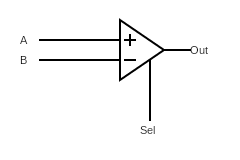
\includegraphics{mux_ext.png}
	\caption{Diagrama externo del circuito MUX} \cite{diagram}
	\label{fig:mux_ext}
\end{figure}
\subsubsection{Esquema interior del circuito}
\begin{figure}[H]
	\centering
	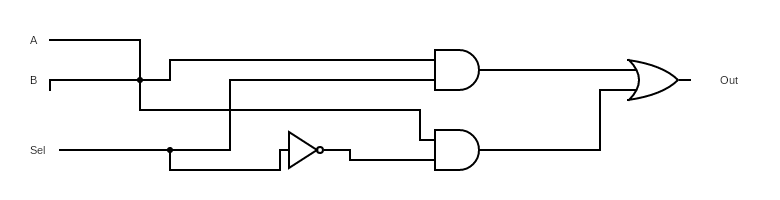
\includegraphics[width=0.5\linewidth]{mux_int.png}
	\caption{Diagrama interior de circuito MUX} \cite{diagram}
	\label{fig:mux_int}
\end{figure}
\subsubsection{Código HDL}

\begin{lstlisting}
	/**
	* Multiplexor:
	* out = a if sel == 0
	*       b otherwise
	*/

	CHIP Mux {
		IN a, b, sel;
		OUT out;

		PARTS:
		Not(in=sel,out=nsel);
		And(a=a,b=nsel,out=c);
		And(a=b,b=sel,out=d);
		Or(a=c,b=d,out=out);
	}
\end{lstlisting}

\newpage
\subsection{DMUX / Demultiplexor}
\subsubsection{Descripción y tabla de verdad}
El demultiplexor (DMUX / DEMUX \cite{floyd_fundamentos_2006}), hace la función contraria del multiplexor; toma datos de una línea y los distribuye a un número determinado de salidas. También se le conoce como distribuidor de datos.

% Please add the following required packages to your document preamble:
% \usepackage{graphicx}
\begin{table}[H]
	\centering
	\caption{Tabla de verdad de DMUX}
	\label{tab:dmux}
	\resizebox{0.25\linewidth}{!}{%
		\begin{tabular}{ll|ll}
			in & sel & A & B \\ \hline
			0  & 0   & 0 & 0 \\
			0  & 1   & 0 & 0 \\
			1  & 0   & 1 & 0 \\
			1  & 1   & 0 & 1
		\end{tabular}%
	}
\end{table}
\subsubsection{Esquema exterior del circuito}
\begin{figure}[H]
	\centering
	\includesvg{dmux_ext.svg}
	\caption{Diagrama externo del circuito DMUX} \cite{diagram}
	\label{fig:dmux_ext}
\end{figure}
\subsubsection{Esquema interior del circuito}
\begin{figure}[H]
	\centering
	\includesvg{dmux_int.svg}
	\caption{Diagrama interno del circuito DMUX} \cite{diagram}
	\label{fig:enter-label}
\end{figure}
\newpage \subsubsection{Código HDL}
\begin{lstlisting}
	/**
	* Demultiplexor:
	* {a, b} = {in, 0} if sel == 0
	*          {0, in} if sel == 1
	*/

	CHIP DMux {
		IN in, sel;
		OUT a, b;

		PARTS:
		Not(in=sel,out=nsel);
		And(a=in,b=nsel,out=a);
		And(a=in,b=sel,out=b);
	}
\end{lstlisting}
\newpage

\section{Not16}
\subsection{Tabla de verdad y explicación del circuito}

Una puerta lógica Not de \textit{N}-Bits, aplica una operación booleana a cada uno de los bits en sus inputs. \cite{nisan_nand2tetris_2005}

\begin{table}[H]
	\centering
	\caption{Tabla de verdad de NOT16}
	\label{tab:tab_not16}
	\resizebox{\textwidth}{!}{%
		\begin{tabular}{@{}ll@{}}
			\toprule
			\texttt{IN}               & \texttt{OUT}              \\ \midrule
			\texttt{0000000000000000} & \texttt{1111111111111111} \\
			\texttt{1111111111111111} & \texttt{0000000000000000} \\
			\texttt{0101010101010101} & \texttt{1010101010101010} \\
			\texttt{. . .}            & \texttt{. . .}            \\ \bottomrule
		\end{tabular}%
	}
\end{table}


\subsection{Esquema del circuito interior}
\begin{figure}[H]
	\centering
	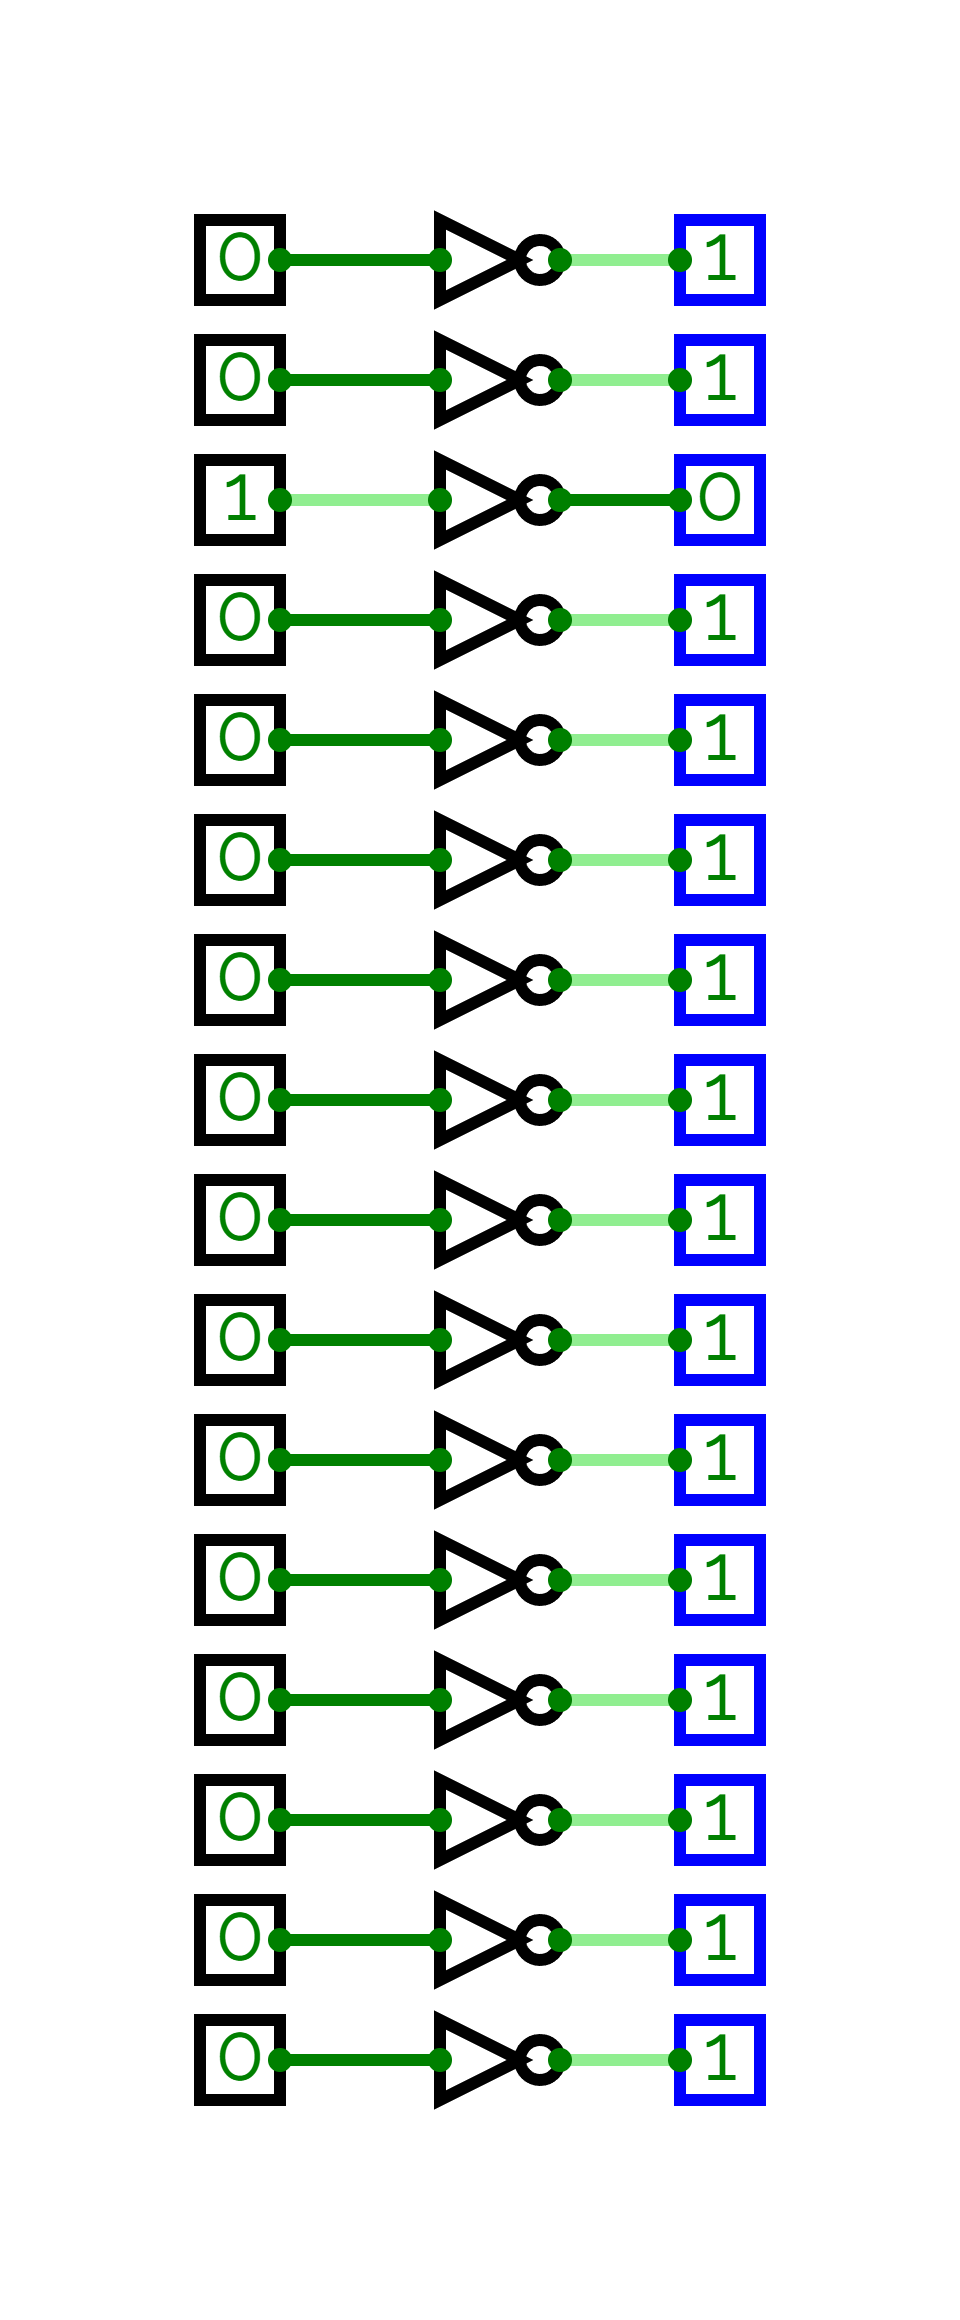
\includegraphics[width=0.4\textwidth]{CIRCUITOS/INT/NOT16_INT.png}
	\caption{Circuito interno de NOT16 \cite{circuitverse}}
	\label{fig:not16_int}
\end{figure}
\subsection{Esquema del circuito exterior}
\begin{figure}[H]
	\centering
	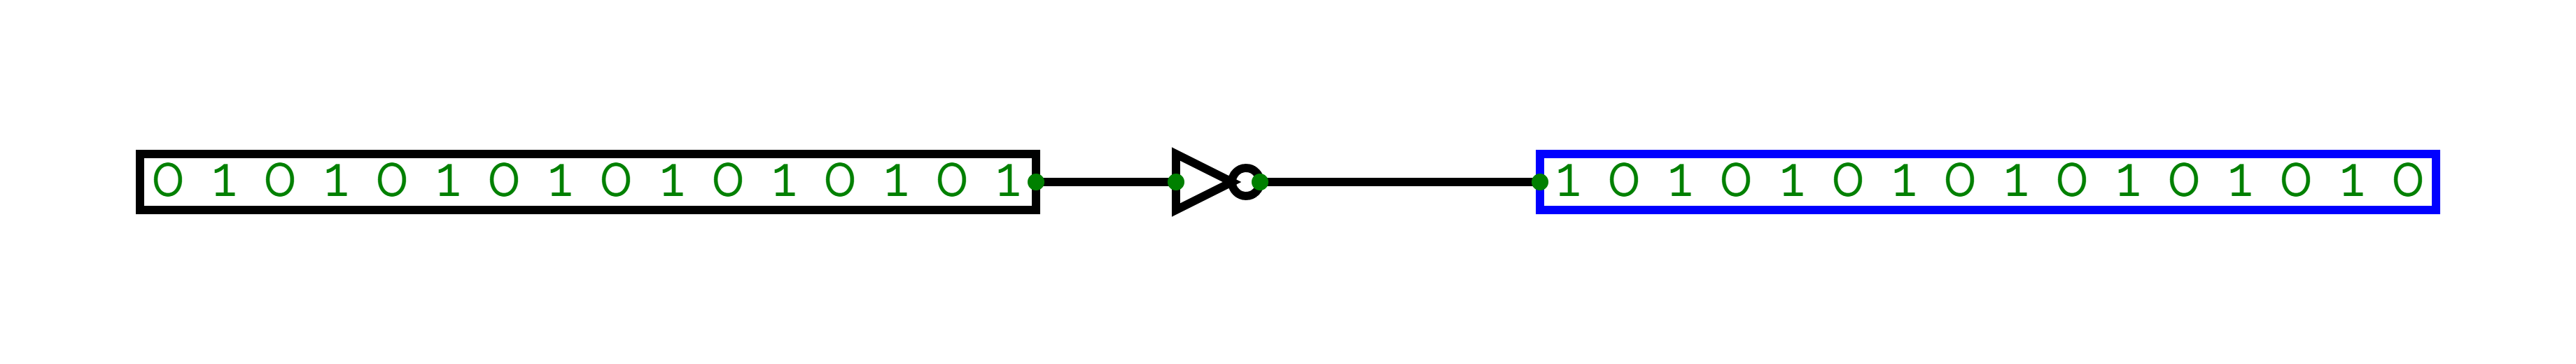
\includegraphics[width=1\textwidth]{CIRCUITOS/EXT/not16_ext.png}
	\caption{Circuito externo de NOT16 \cite{circuitverse}}
	\label{fig:not16_ext}
\end{figure}
\subsection{Implementación HDL}
\begin{figure}[H]
	\centering
	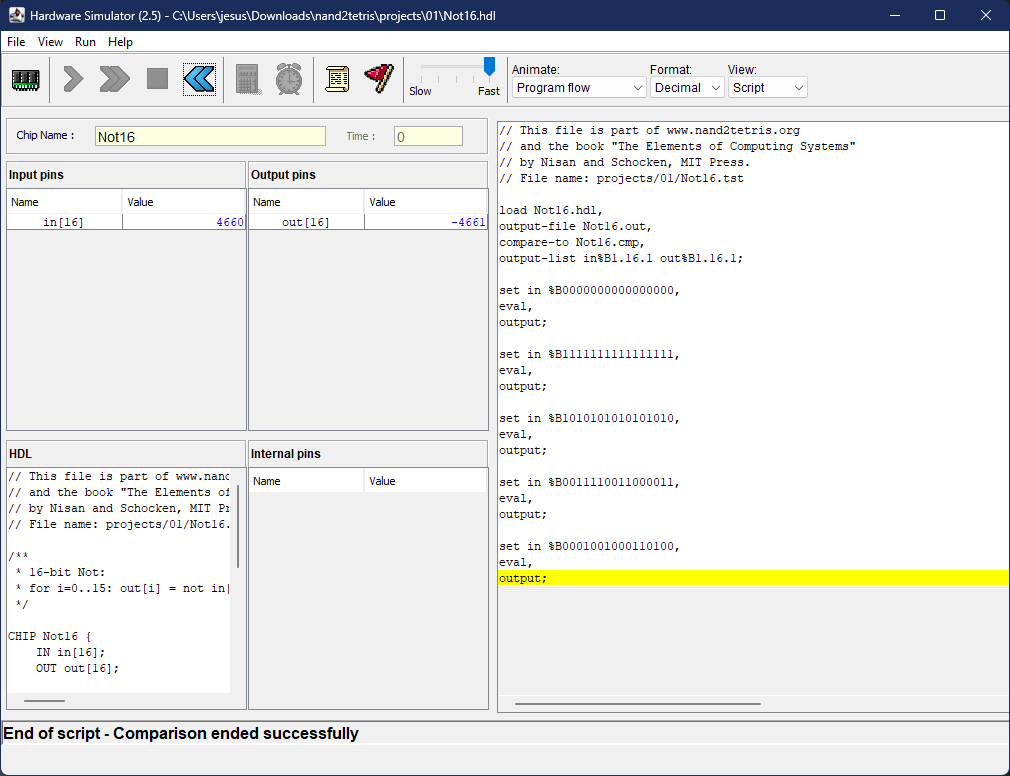
\includegraphics[width=0.75\textwidth]{CIRCUITOS/HDL/not16hdl.png}
	\caption{Test en Hardware Simulator de NOT16 \cite{nand2tetris}}
	\label{fig:hdlnot16}
\end{figure}

\subsubsection{Archivo HDL}
\begin{lstlisting}
	CHIP Not16 {
		IN in[16];
		OUT out[16];

		PARTS:
		Not(in=in[0], out=out[0]);
		Not(in=in[1], out=out[1]);
		Not(in=in[2], out=out[2]);
		Not(in=in[3], out=out[3]);
		Not(in=in[4], out=out[4]);
		Not(in=in[5], out=out[5]);
		Not(in=in[6], out=out[6]);
		Not(in=in[7], out=out[7]);
		Not(in=in[8], out=out[8]);
		Not(in=in[9], out=out[9]);
		Not(in=in[10], out=out[10]);
		Not(in=in[11], out=out[11]);
		Not(in=in[12], out=out[12]);
		Not(in=in[13], out=out[13]);
		Not(in=in[14], out=out[14]);
		Not(in=in[15], out=out[15]);
	}
\end{lstlisting}
\newpage

%%%%%%%%%%%%%%%%%%%%%%%%%%%%%%%%%%%%%%%%%%%%%%%%%%%%%%%%%%%%%%%%%%%%%%%%%%
%%%%%%%%%%%%%%%%%%%%%%%%%%%%%%%%%%%%%%%%%%%%%%%%%%%%%%%%%%%%%%%%%%%%%%%%%%

\section{And16}
Una puerta lógica de \textit{N}-bits And aplica una operación a cada uno de \textit{N}-pares conectados a sus dos buses inputs de \textit{N}-bits. \cite{nisan_nand2tetris_2005}
\subsection{Tabla de verdad y explicación del circuito}
\begin{table}[H]
	\centering
	\caption{Tabla de verdad de AND16}
	\label{tab:tab_and16}
	\resizebox{\textwidth}{!}{%
		\begin{tabular}{@{}lll@{}}
			\toprule
			\texttt{a}                & \texttt{b}                & \texttt{out}              \\ \midrule
			\texttt{0000000000000000} & \texttt{0000000000000000} & \texttt{0000000000000000} \\
			\texttt{0000000000000000} & \texttt{1111111111111111} & \texttt{0000000000000000} \\
			\texttt{1111111111111111} & \texttt{1111111111111111} & \texttt{1111111111111111} \\
			\texttt{1010101010101010} & \texttt{0101010101010101} & \texttt{0000000000000000} \\
			\texttt{0011110011000011} & \texttt{0000111111110000} & \texttt{0000110011000000} \\
			\texttt{0001001000110100} & \texttt{1001100001110110} & \texttt{0001000000110100} \\ \bottomrule
		\end{tabular}%
	}
\end{table}

\subsection{Esquema del circuito interior}
\begin{figure}[H]
	\centering
	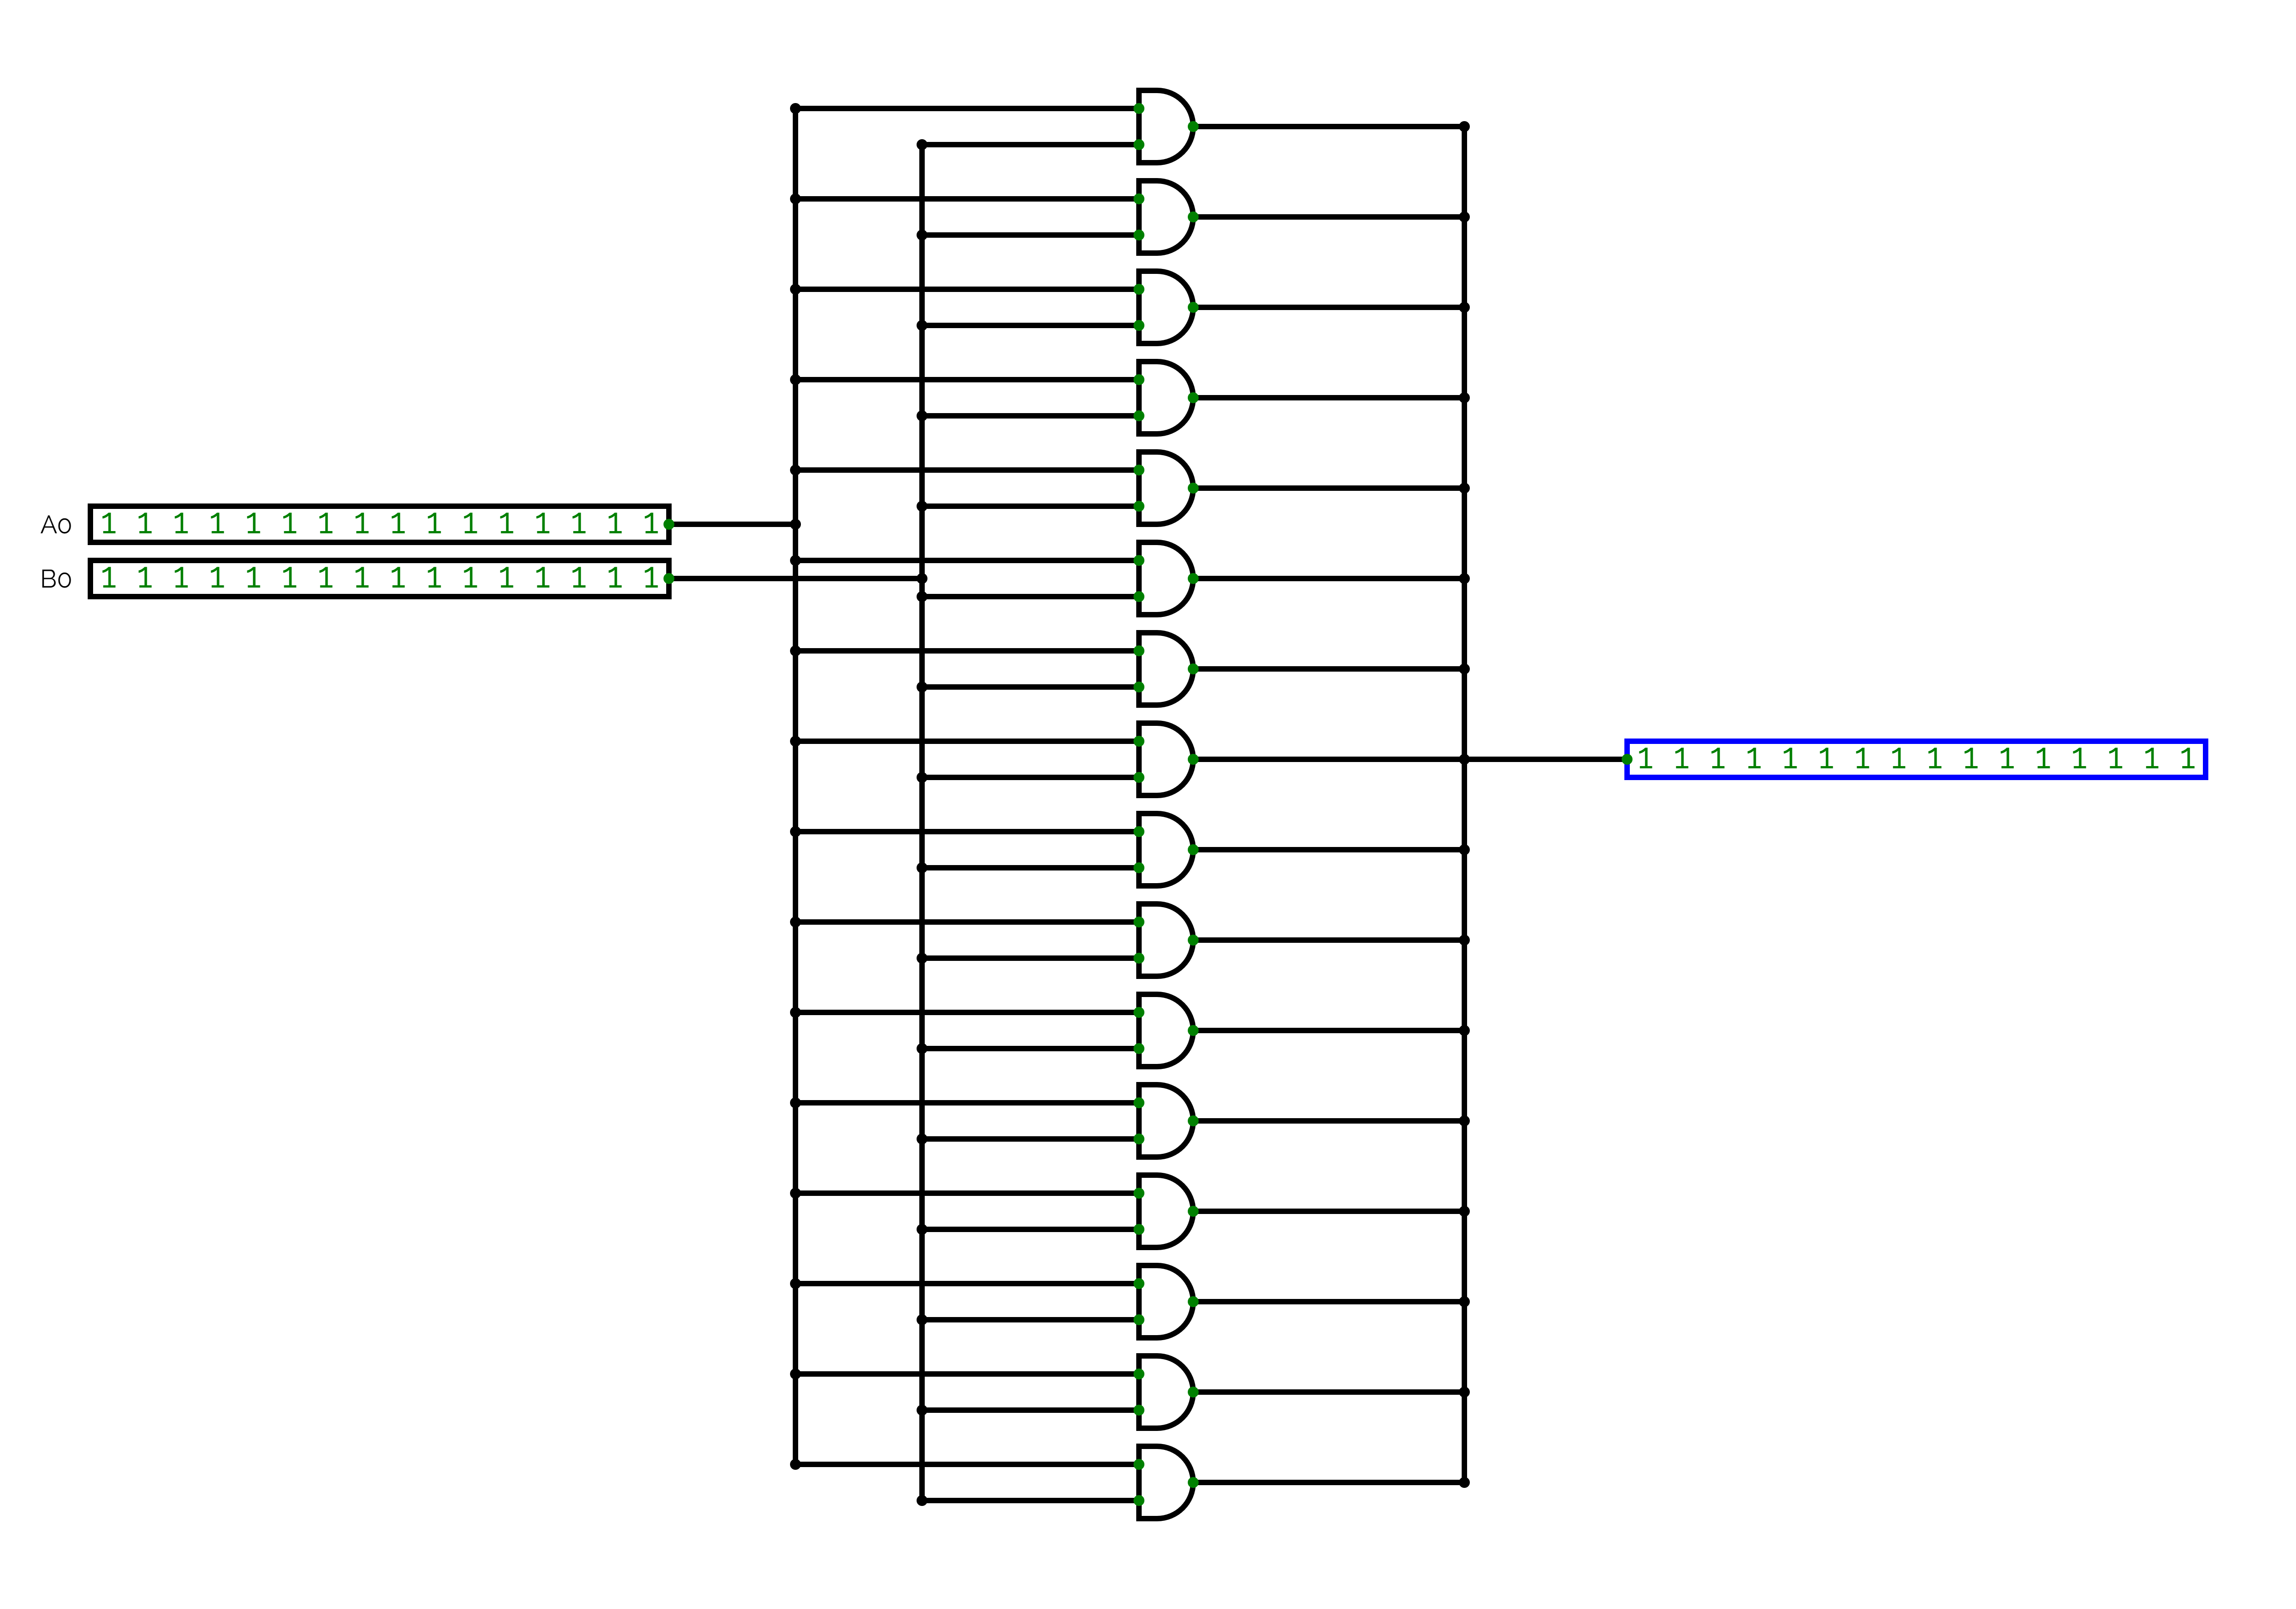
\includegraphics[width=\linewidth]{CIRCUITOS/INT/And16_int.png}
	\caption{Circuito interior de And16 \cite{circuitverse}}
	\label{fig:and16_int}
\end{figure}
\subsection{Esquema del circuito exterior}
\begin{figure}[H]
	\centering
	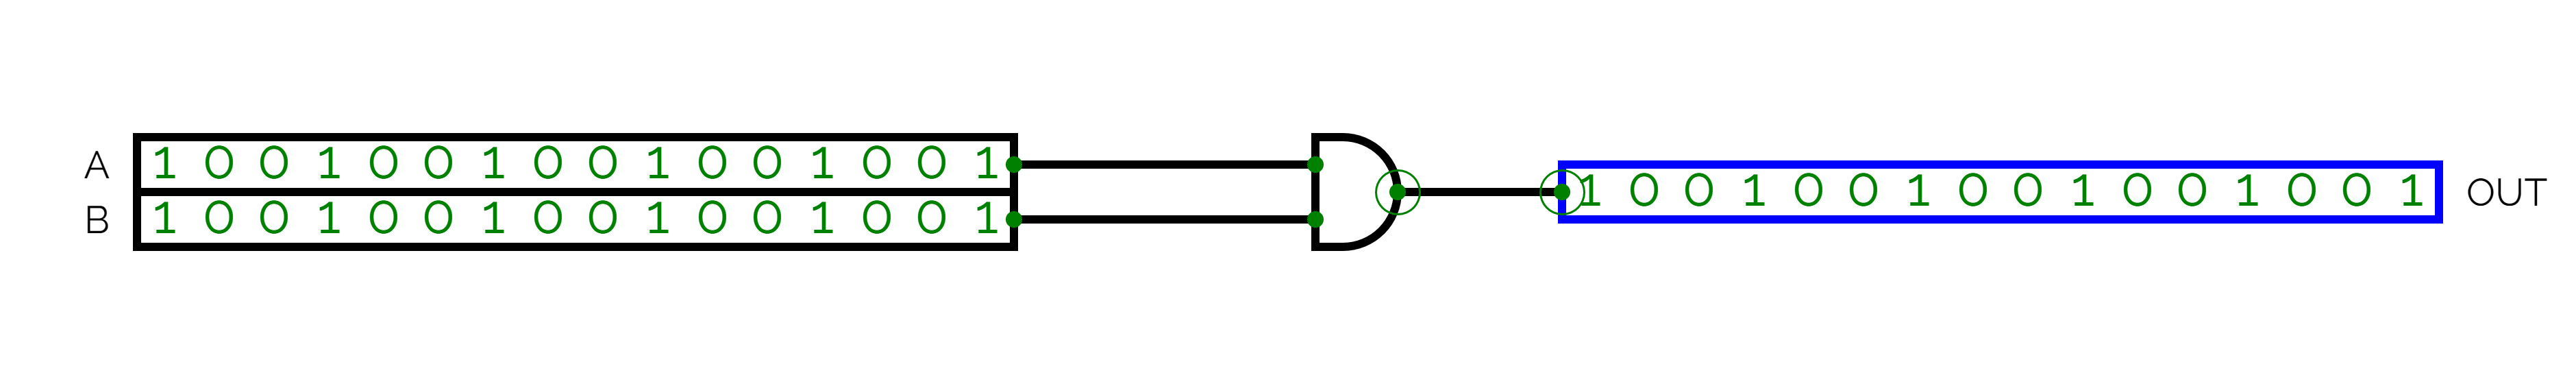
\includegraphics[width=\linewidth]{CIRCUITOS/EXT/and16_ext.png}
	\caption{Circuito exterior de And16 \cite{circuitverse}}
	\label{fig:and16_ext}
\end{figure}
\subsection{Implementación HDL}
\begin{figure}[H]
	\centering
	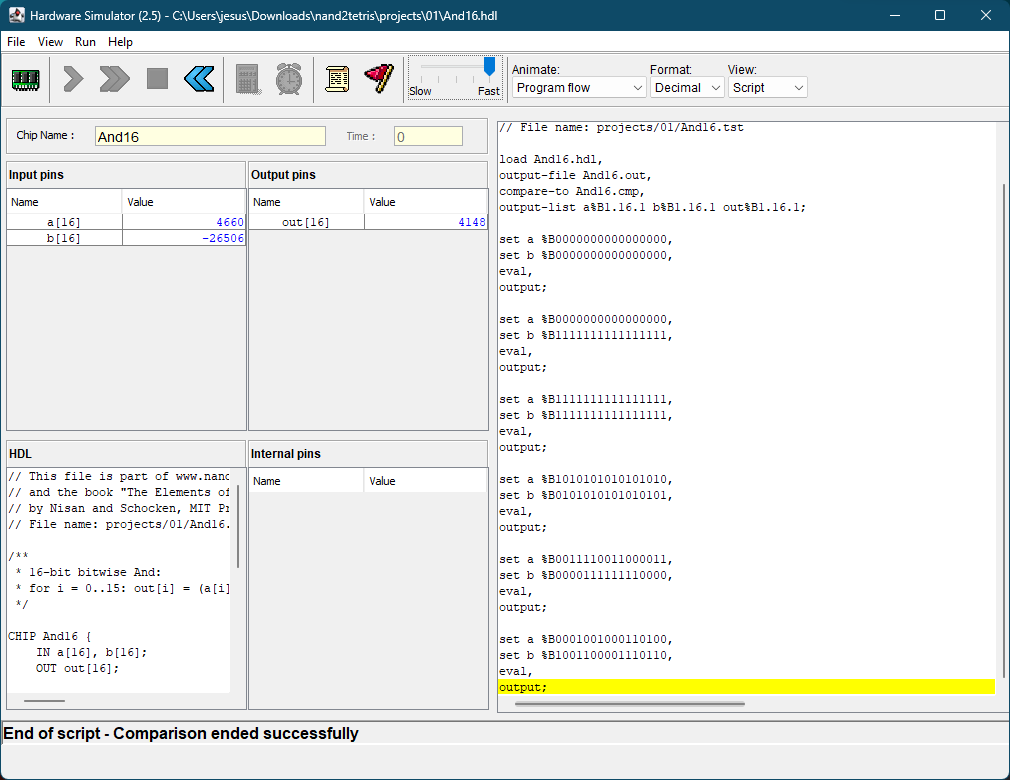
\includegraphics[width=0.75\linewidth]{CIRCUITOS/HDL/and16hdl.png}
	\caption{Test en Hardware Simulator de And16 \cite{nand2tetris}}
	\label{fig:hdland16}
\end{figure}
\subsubsection{Archivo HDL}
\begin{lstlisting}
	CHIP And16 {
		IN a[16], b[16];
		OUT out[16];

		PARTS:
		And(a=a[0],b=b[0], out=out[0]);
		And(a=a[1],b=b[1], out=out[1]);
		And(a=a[2],b=b[2], out=out[2]);
		And(a=a[3],b=b[3], out=out[3]);
		And(a=a[4],b=b[4], out=out[4]);
		And(a=a[5],b=b[5], out=out[5]);
		And(a=a[6],b=b[6], out=out[6]);
		And(a=a[7],b=b[7], out=out[7]);
		And(a=a[8],b=b[8], out=out[8]);
		And(a=a[9],b=b[9], out=out[9]);
		And(a=a[10],b=b[10],out=out[10]);
		And(a=a[11],b=b[11],out=out[11]);
		And(a=a[12],b=b[12],out=out[12]);
		And(a=a[13],b=b[13],out=out[13]);
		And(a=a[14],b=b[14],out=out[14]);
		And(a=a[15],b=b[15],out=out[15]);
	}
\end{lstlisting}
\newpage

%%%%%%%%%%%%%%%%%%%%%%%%%%%%%%%%%%%%%%%%%%%%%%%%%%%%%%%%%%%%%%%%%%%%%%%%%%
%%%%%%%%%%%%%%%%%%%%%%%%%%%%%%%%%%%%%%%%%%%%%%%%%%%%%%%%%%%%%%%%%%%%%%%%%%

\section{Or16}
\subsection{Tabla de verdad y explicación del circuito}
La puerta lógica Or de \textit{N}-bits aplica una operación booleana de tipo Or a cada uno de sus inputs pares de \textit{N}-bits. \cite{nisan_nand2tetris_2005}
\begin{table}[H]
	\centering
	\caption{Tabla de verdad de OR16}
	\label{tab:tab_or16}
	\resizebox{\textwidth}{!}{%
		\begin{tabular}{@{}lll@{}}
			\toprule
			\texttt{a}                & \texttt{b}                & \texttt{out}              \\ \midrule
			\texttt{0000000000000000} & \texttt{0000000000000000} & \texttt{0000000000000000} \\
			\texttt{0000000000000000} & \texttt{1111111111111111} & \texttt{1111111111111111} \\
			\texttt{1111111111111111} & \texttt{1111111111111111} & \texttt{1111111111111111} \\
			\texttt{1010101010101010} & \texttt{0101010101010101} & \texttt{1111111111111111} \\
			\texttt{0011110011000011} & \texttt{0000111111110000} & \texttt{0011111111110011} \\
			\texttt{0001001000110100} & \texttt{1001100001110110} & \texttt{1001101001110110} \\ \bottomrule
		\end{tabular}%
	}
\end{table}

\subsection{Esquema del circuito interior}
\begin{figure}[H]
	\centering
	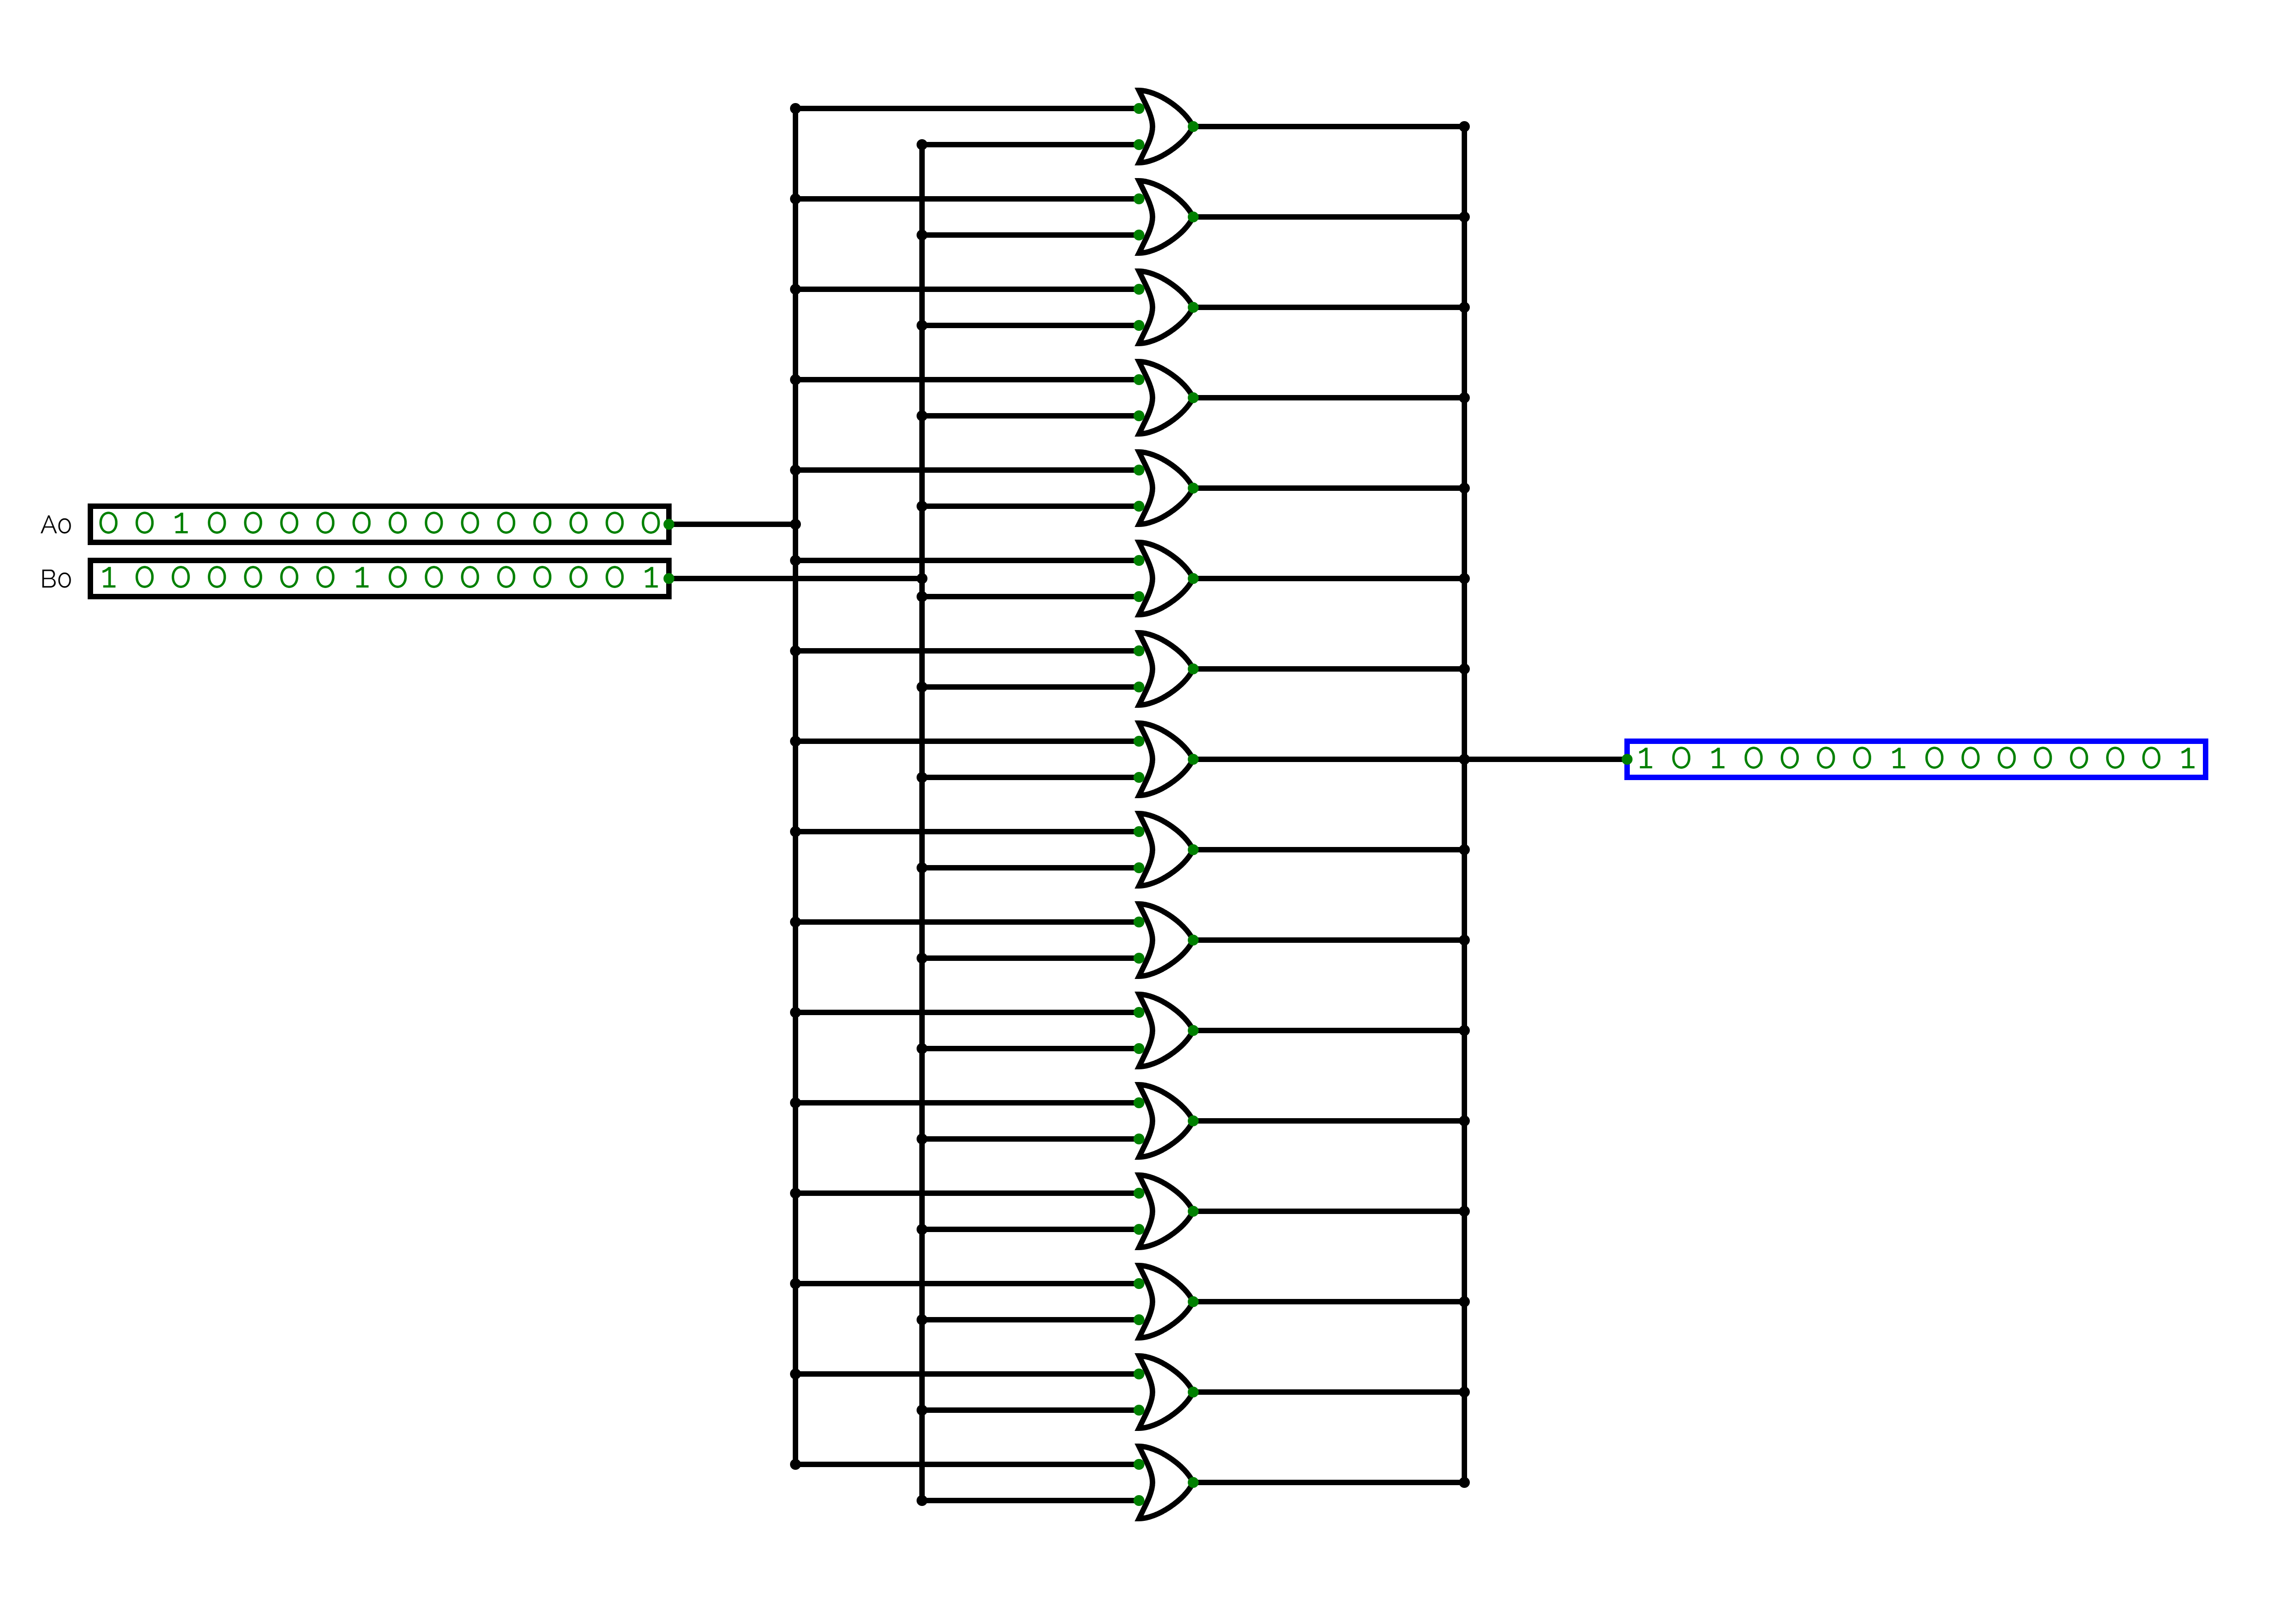
\includegraphics[width=1\textwidth]{CIRCUITOS/INT/OR16_int.png}
	\caption{Circuito interior de Or16 \cite{circuitverse}}
	\label{fig:or16_int}
\end{figure}
\subsection{Esquema del circuito exterior}
\begin{figure}[H]
	\centering
	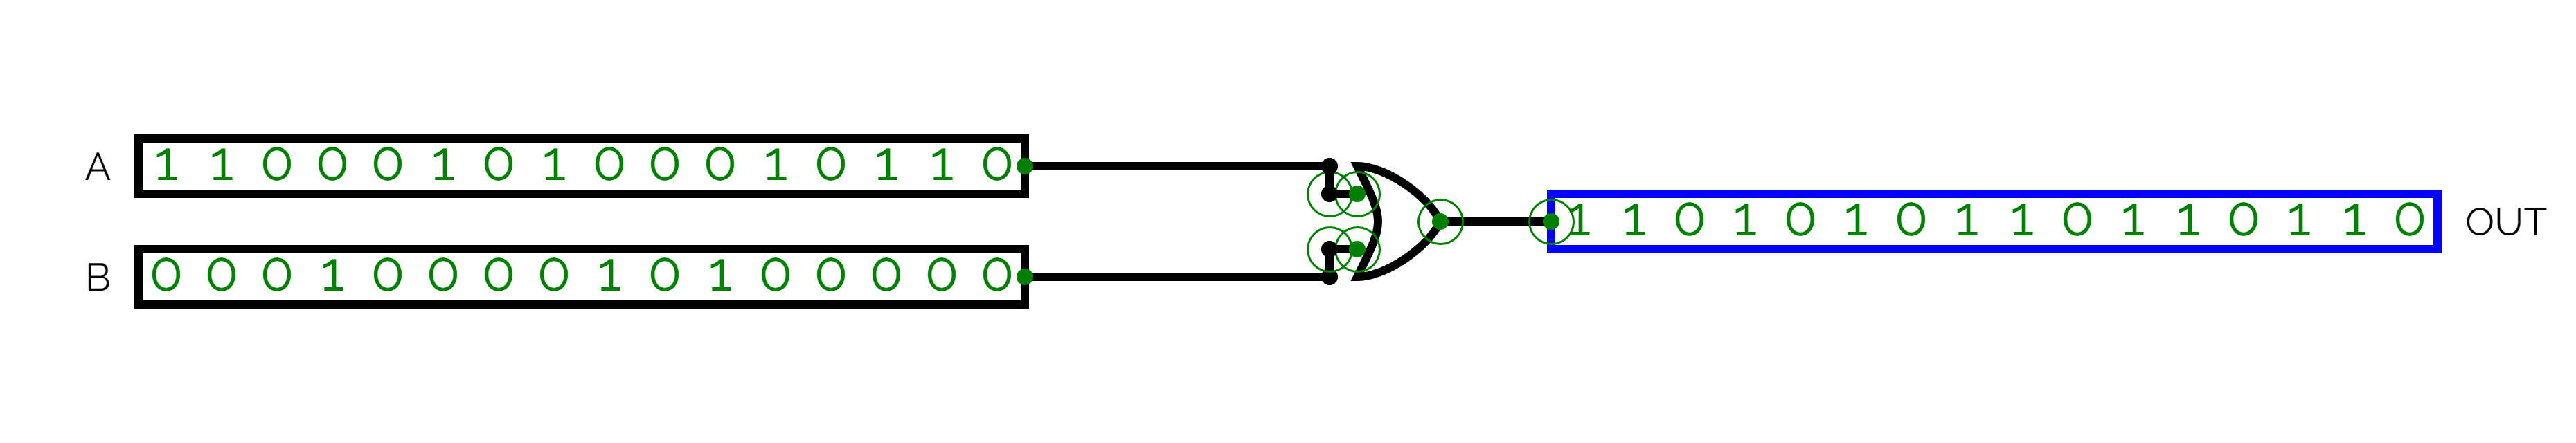
\includegraphics[width=1\textwidth]{CIRCUITOS/EXT/OR16_ext.png}
	\caption{Circuito exterior de Or16 \cite{circuitverse}}
	\label{fig:or16_ext}
\end{figure}
\subsection{Implementación HDL}
\begin{figure}[H]
	\centering
	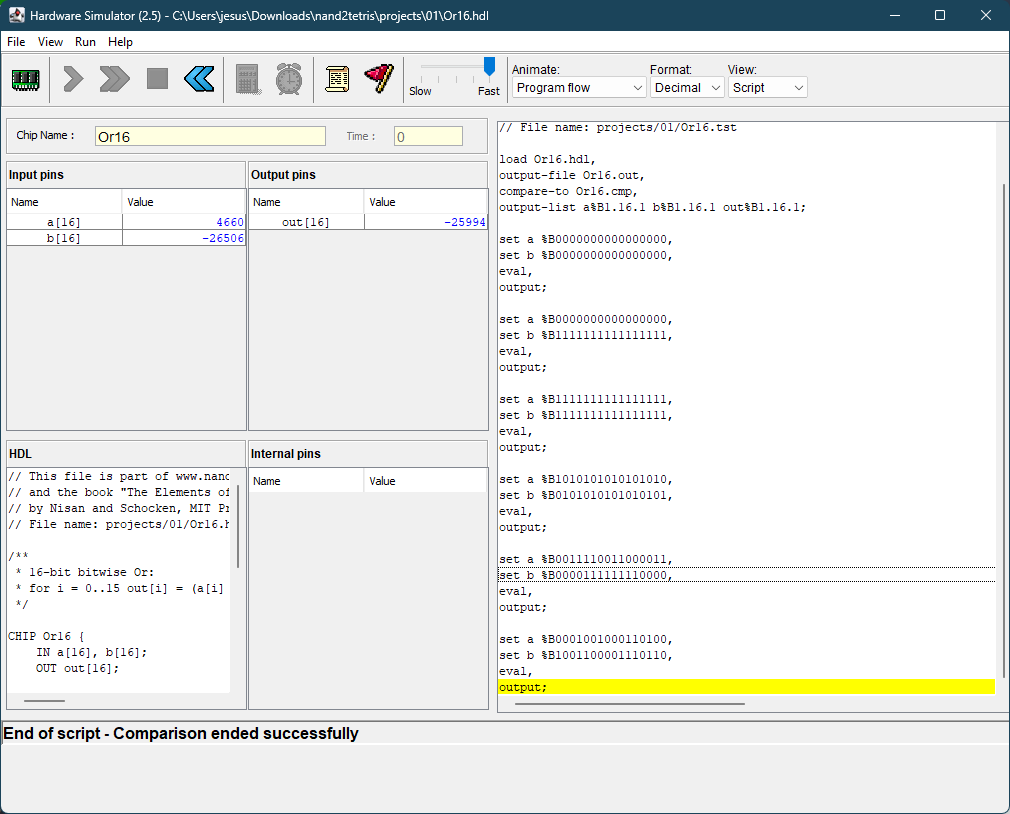
\includegraphics[width=0.75\linewidth]{CIRCUITOS//HDL/or16hdl.png}
	\caption{Test en Hardware Simulator de Or16 \cite{nand2tetris}}
	\label{fig:hdlor16}
\end{figure}
\subsubsection{Archivo HDL}
\begin{lstlisting}
	CHIP Or16 {
		IN a[16], b[16];
		OUT out[16];

		PARTS:
		Or(a=a[0], b=b[0], out=out[0]);
		Or(a=a[1], b=b[1], out=out[1]);
		Or(a=a[2], b=b[2], out=out[2]);
		Or(a=a[3], b=b[3], out=out[3]);
		Or(a=a[4], b=b[4], out=out[4]);
		Or(a=a[5], b=b[5], out=out[5]);
		Or(a=a[6], b=b[6], out=out[6]);
		Or(a=a[7], b=b[7], out=out[7]);
		Or(a=a[8], b=b[8], out=out[8]);
		Or(a=a[9], b=b[9], out=out[9]);
		Or(a=a[10], b=b[10], out=out[10]);
		Or(a=a[11], b=b[11], out=out[11]);
		Or(a=a[12], b=b[12], out=out[12]);
		Or(a=a[13], b=b[13], out=out[13]);
		Or(a=a[14], b=b[14], out=out[14]);
		Or(a=a[15], b=b[15], out=out[15]);
	}
\end{lstlisting}
\newpage

%%%%%%%%%%%%%%%%%%%%%%%%%%%%%%%%%%%%%%%%%%%%%%%%%%%%%%%%%%%%%%%%%%%%%%%%%%
%%%%%%%%%%%%%%%%%%%%%%%%%%%%%%%%%%%%%%%%%%%%%%%%%%%%%%%%%%%%%%%%%%%%%%%%%%

\section{Mux16}
\subsection{Tabla de verdad y explicación del circuito}
Un multiplexador (Mux\textit{X}bits) de \textit{N}-bits, se comporta de manera parecida a un Mux exceptuando en que sus dos inputs son de \textit{N}-bits de ancho (16 en este caso). \cite{nisan_nand2tetris_2005}
\begin{table}[H]
	\centering
	\caption{Tabla de verdad de MUX16}
	\label{tab:tab_mux16}
	\resizebox{\columnwidth}{!}{%
		\begin{tabular}{@{}llll@{}}
			\toprule
			\texttt{a}                & \texttt{b}                & \texttt{sel} & \texttt{out}              \\ \midrule
			\texttt{0000000000000000} & \texttt{0000000000000000} & \texttt{0}   & \texttt{0000000000000000} \\
			\texttt{0000000000000000} & \texttt{0000000000000000} & \texttt{1}   & \texttt{0000000000000000} \\
			\texttt{0000000000000000} & \texttt{0001001000110100} & \texttt{0}   & \texttt{0000000000000000} \\
			\texttt{0000000000000000} & \texttt{0001001000110100} & \texttt{1}   & \texttt{0001001000110100} \\
			\texttt{1001100001110110} & \texttt{0000000000000000} & \texttt{0}   & \texttt{1001100001110110} \\
			\texttt{1001100001110110} & \texttt{0000000000000000} & \texttt{1}   & \texttt{0000000000000000} \\
			\texttt{1010101010101010} & \texttt{0101010101010101} & \texttt{0}   & \texttt{1010101010101010} \\
			\texttt{1010101010101010} & \texttt{0101010101010101} & \texttt{1}   & \texttt{0101010101010101} \\ \bottomrule
		\end{tabular}%
	}
\end{table}

\subsection{Esquema del circuito interior}
\begin{figure}[H]
	\centering
	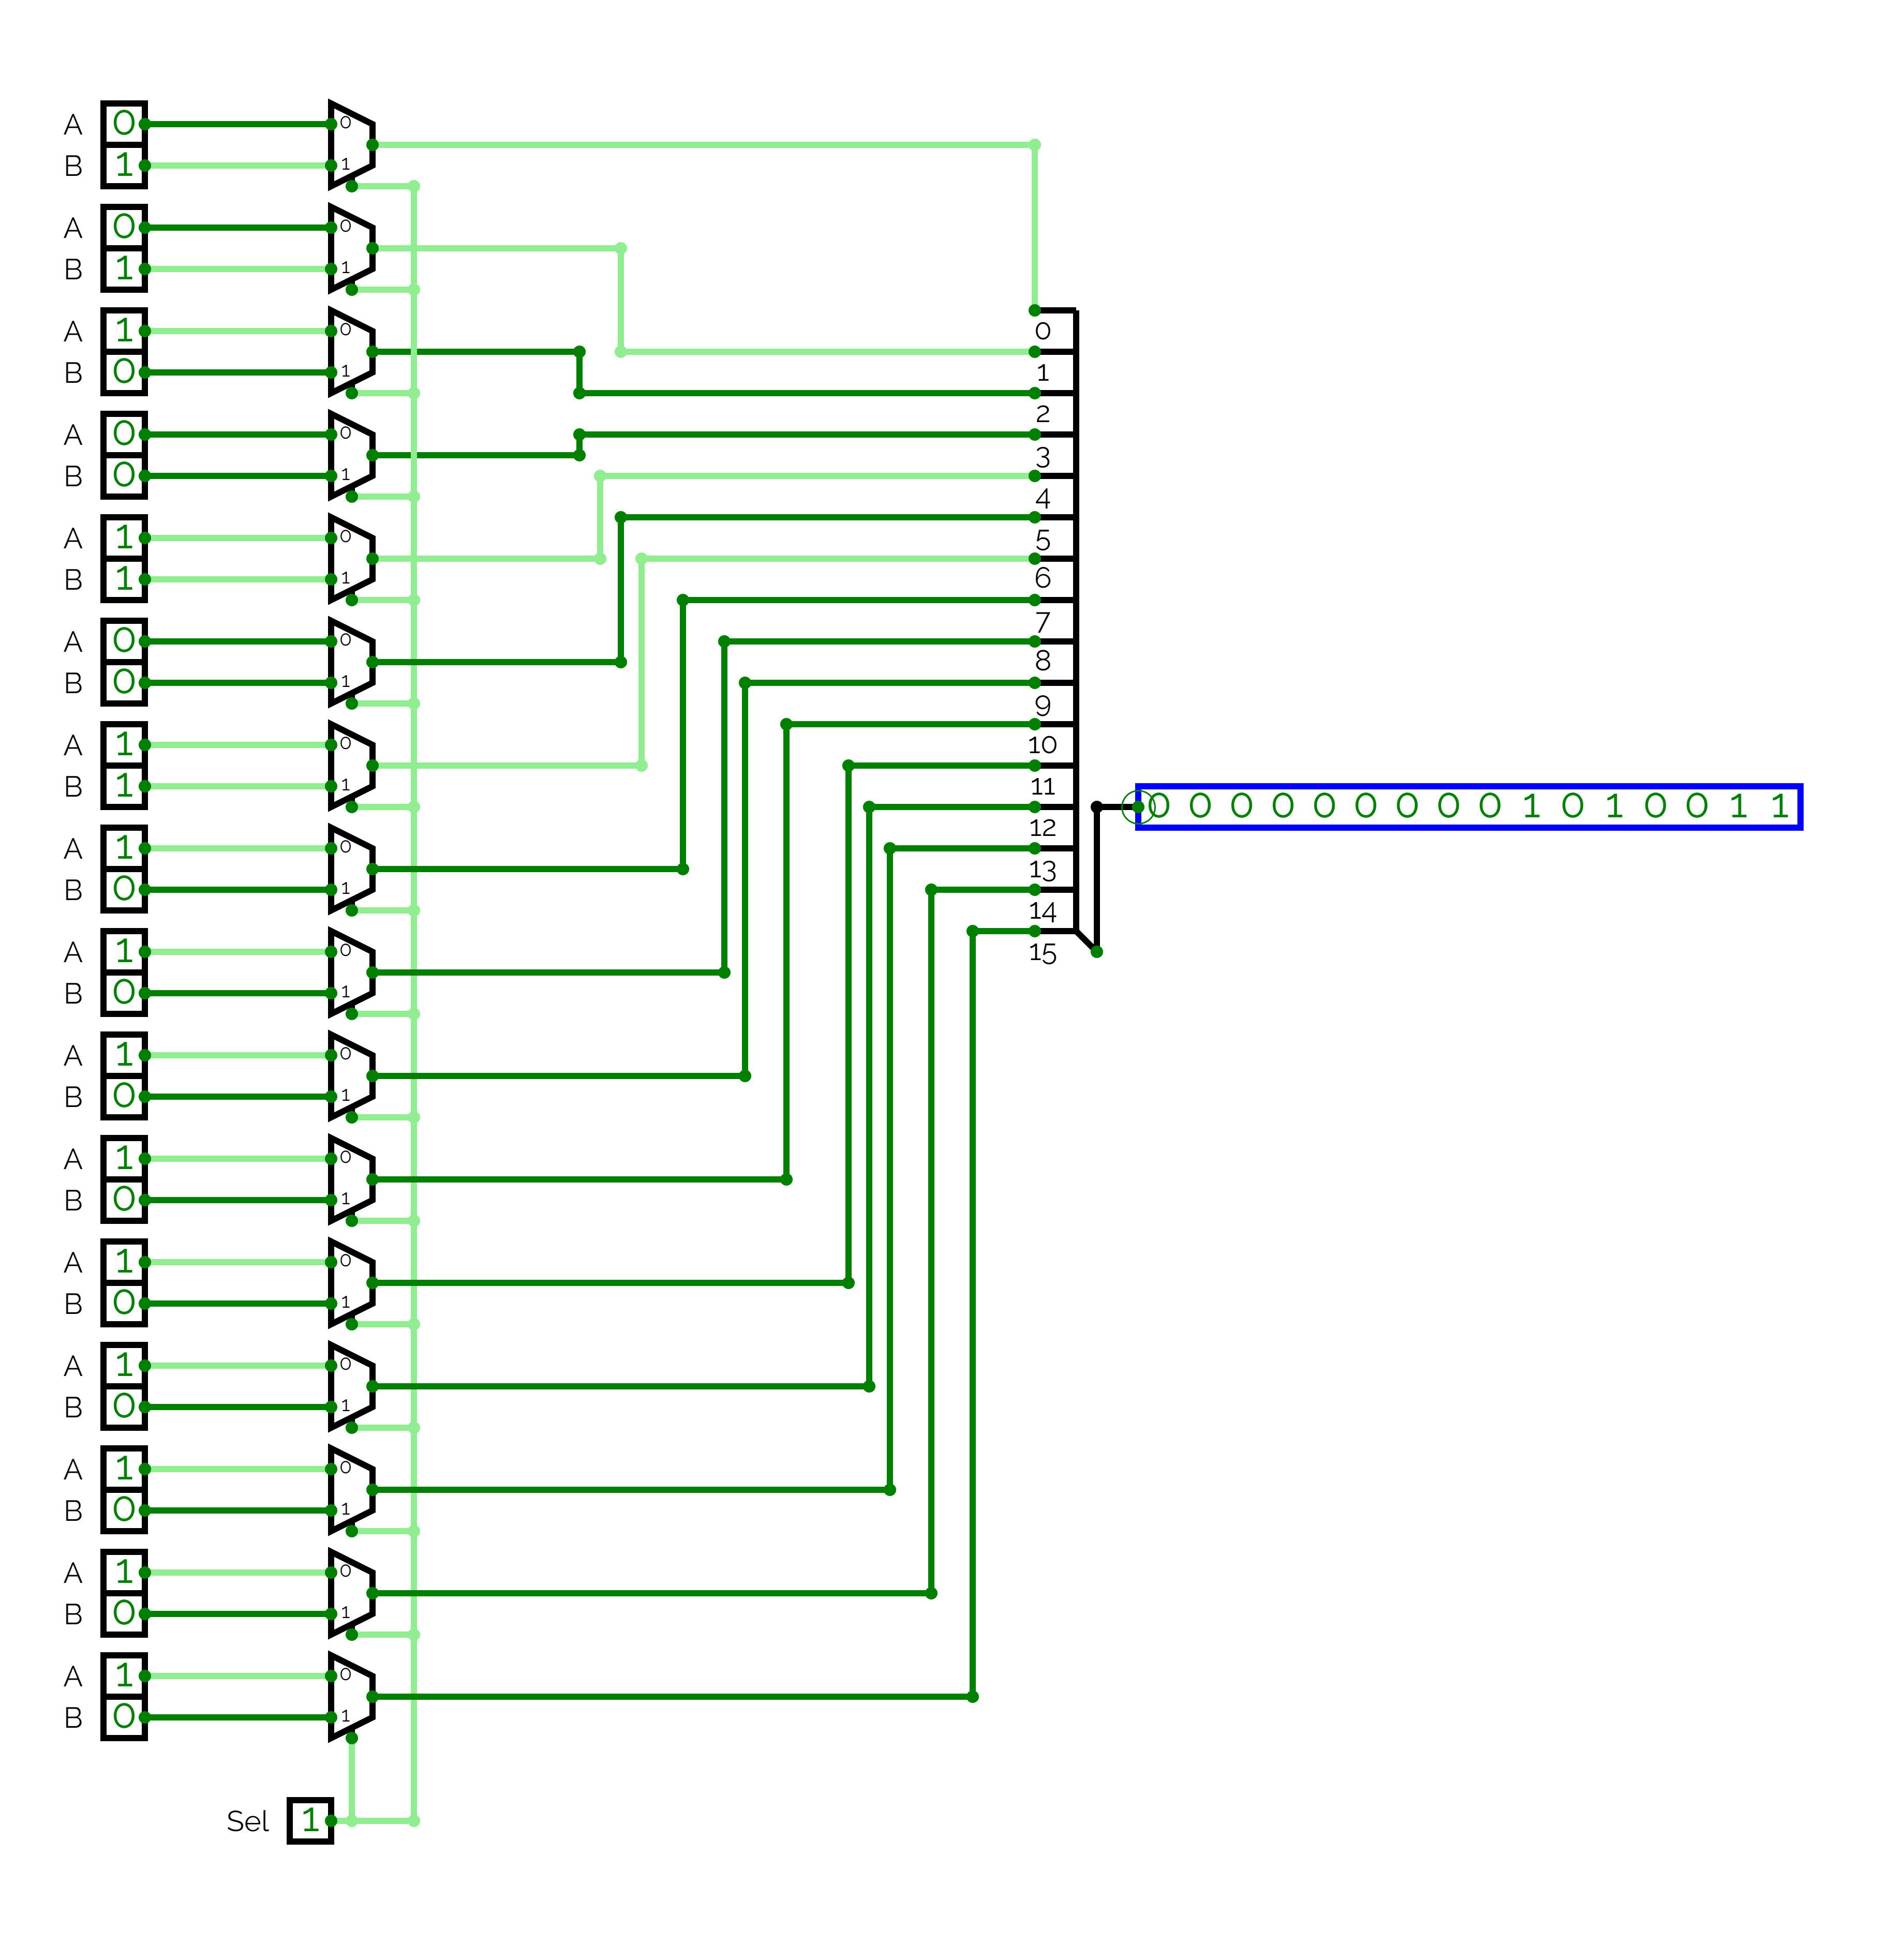
\includegraphics[width=1\textwidth]{CIRCUITOS/INT/Mux16_int.png}
	\caption{Circuito interior de Mux16 \cite{circuitverse}}
	\label{fig:mux16_int}
\end{figure}
\subsection{Esquema del circuito exterior}
\begin{figure}[H]
	\centering
	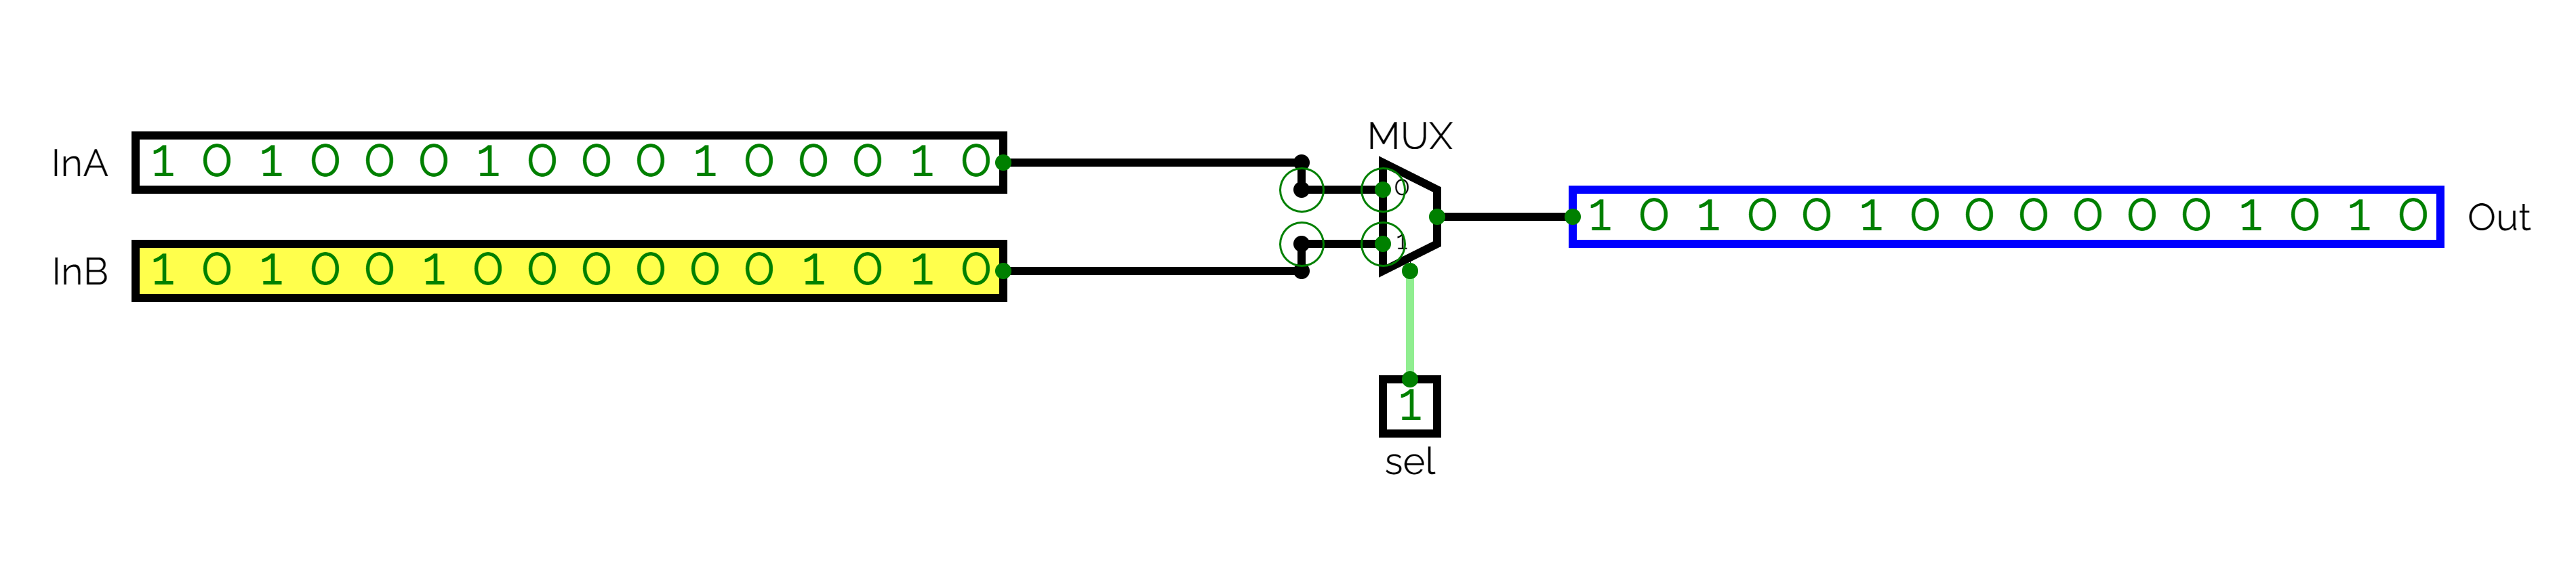
\includegraphics[width=1\textwidth]{CIRCUITOS/EXT/Mux16_ext1.png}
	\caption{Circuito exterior de Mux16 \cite{circuitverse}}
	\label{fig:mux16_ext}
\end{figure}
\subsection{Implementación HDL}
\begin{figure}[H]
	\centering
	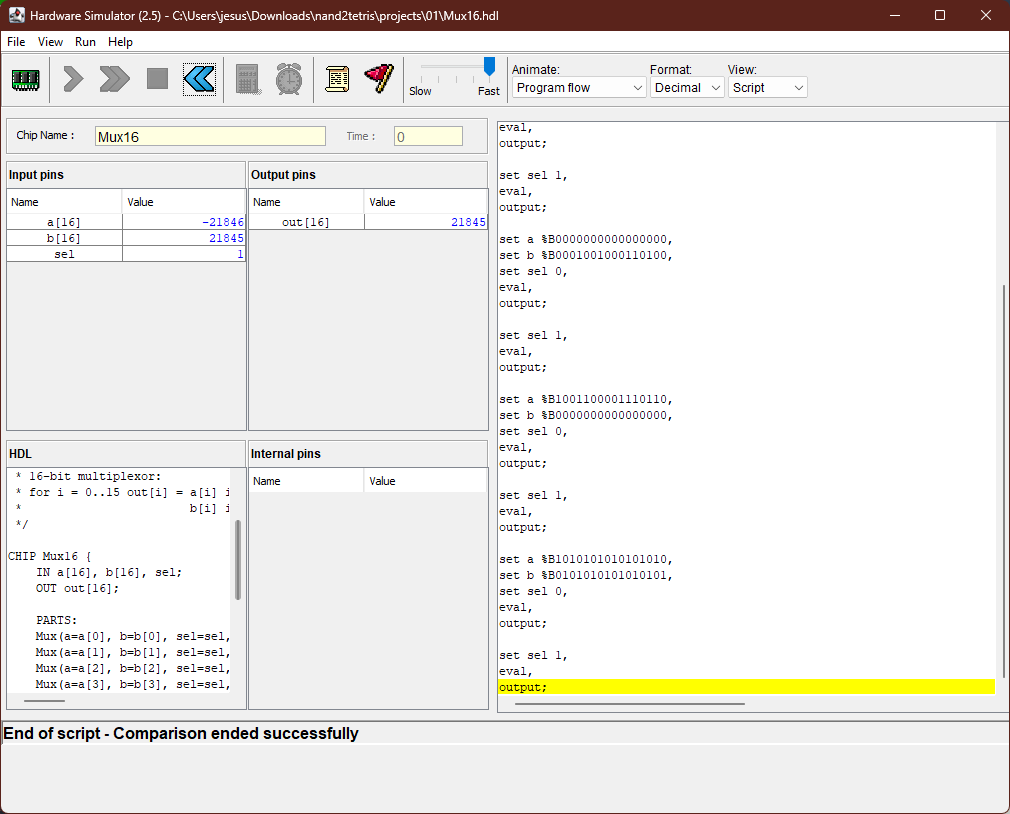
\includegraphics[width=0.75\linewidth]{CIRCUITOS//HDL/mux16hdl.png}
	\caption{Test en Hardware Simulator de Mux16 \cite{nand2tetris}}
	\label{fig:hdlmux16}
\end{figure}
\subsubsection{Archivo HDL}
\begin{lstlisting}

	CHIP Mux16 {
		IN a[16], b[16], sel;
		OUT out[16];

		PARTS:
		Mux(a=a[0], b=b[0], sel=sel, out=out[0]);
		Mux(a=a[1], b=b[1], sel=sel, out=out[1]);
		Mux(a=a[2], b=b[2], sel=sel, out=out[2]);
		Mux(a=a[3], b=b[3], sel=sel, out=out[3]);
		Mux(a=a[4], b=b[4], sel=sel, out=out[4]);
		Mux(a=a[5], b=b[5], sel=sel, out=out[5]);
		Mux(a=a[6], b=b[6], sel=sel, out=out[6]);
		Mux(a=a[7], b=b[7], sel=sel, out=out[7]);
		Mux(a=a[8], b=b[8], sel=sel, out=out[8]);
		Mux(a=a[9], b=b[9], sel=sel, out=out[9]);
		Mux(a=a[10], b=b[10], sel=sel, out=out[10]);
		Mux(a=a[11], b=b[11], sel=sel, out=out[11]);
		Mux(a=a[12], b=b[12], sel=sel, out=out[12]);
		Mux(a=a[13], b=b[13], sel=sel, out=out[13]);
		Mux(a=a[14], b=b[14], sel=sel, out=out[14]);
		Mux(a=a[15], b=b[15], sel=sel, out=out[15]);
	}
\end{lstlisting}
\newpage

%%%%%%%%%%%%%%%%%%%%%%%%%%%%%%%%%%%%%%%%%%%%%%%%%%%%%%%%%%%%%%%%%%%%%%%%%%
%%%%%%%%%%%%%%%%%%%%%%%%%%%%%%%%%%%%%%%%%%%%%%%%%%%%%%%%%%%%%%%%%%%%%%%%%%

\section{DMux4Way (DMuxi1o4b1)} \label{dmux4label}
\subsection{Tabla de verdad y explicación del circuito}
Un demultiplexador de \textit{M}-vías y \textit{N}-bits guía a 1 bit desde su input de un 1 bit, hasta uno de los posibles outputs de \textit{N}-bits. Cuya selección se realiza mediante una colección de bits \textit{k}, cuya fórmula es $k = log_{2}m$. \label{dmux4text} \cite{nisan_nand2tetris_2005}
\begin{table}[H]
	\centering
	\caption{Tabla de verdad de DMUX4WAY}
	\label{tab:tab_dmux4way}
	\resizebox{0.9\columnwidth}{!}{%
		\begin{tabular}{@{}llllll@{}}
			\toprule
			\texttt{in} & \texttt{sel} & \texttt{a} & \texttt{b} & \texttt{c} & \texttt{d} \\ \midrule
			\texttt{0}  & \texttt{00}  & \texttt{0} & \texttt{0} & \texttt{0} & \texttt{0} \\
			\texttt{0}  & \texttt{01}  & \texttt{0} & \texttt{0} & \texttt{0} & \texttt{0} \\
			\texttt{0}  & \texttt{10}  & \texttt{0} & \texttt{0} & \texttt{0} & \texttt{0} \\
			\texttt{0}  & \texttt{11}  & \texttt{0} & \texttt{0} & \texttt{0} & \texttt{0} \\
			\texttt{1}  & \texttt{00}  & \texttt{1} & \texttt{0} & \texttt{0} & \texttt{0} \\
			\texttt{1}  & \texttt{01}  & \texttt{0} & \texttt{1} & \texttt{0} & \texttt{0} \\
			\texttt{1}  & \texttt{10}  & \texttt{0} & \texttt{0} & \texttt{1} & \texttt{0} \\
			\texttt{1}  & \texttt{11}  & \texttt{0} & \texttt{0} & \texttt{0} & \texttt{1} \\ \bottomrule
		\end{tabular}%
	}
\end{table}

\subsection{Esquema del circuito interior}
\begin{figure}[H]
	\centering
	\includegraphics[width=1\textwidth]{CIRCUITOS/INT/Dmux4way_int.png}
	\caption{Circuito interior de DMux4Way \cite{circuitverse}}
	\label{fig:dmux4way_int}
\end{figure}

\subsection{Esquema del circuito exterior}
\begin{figure}[H]
	\centering
	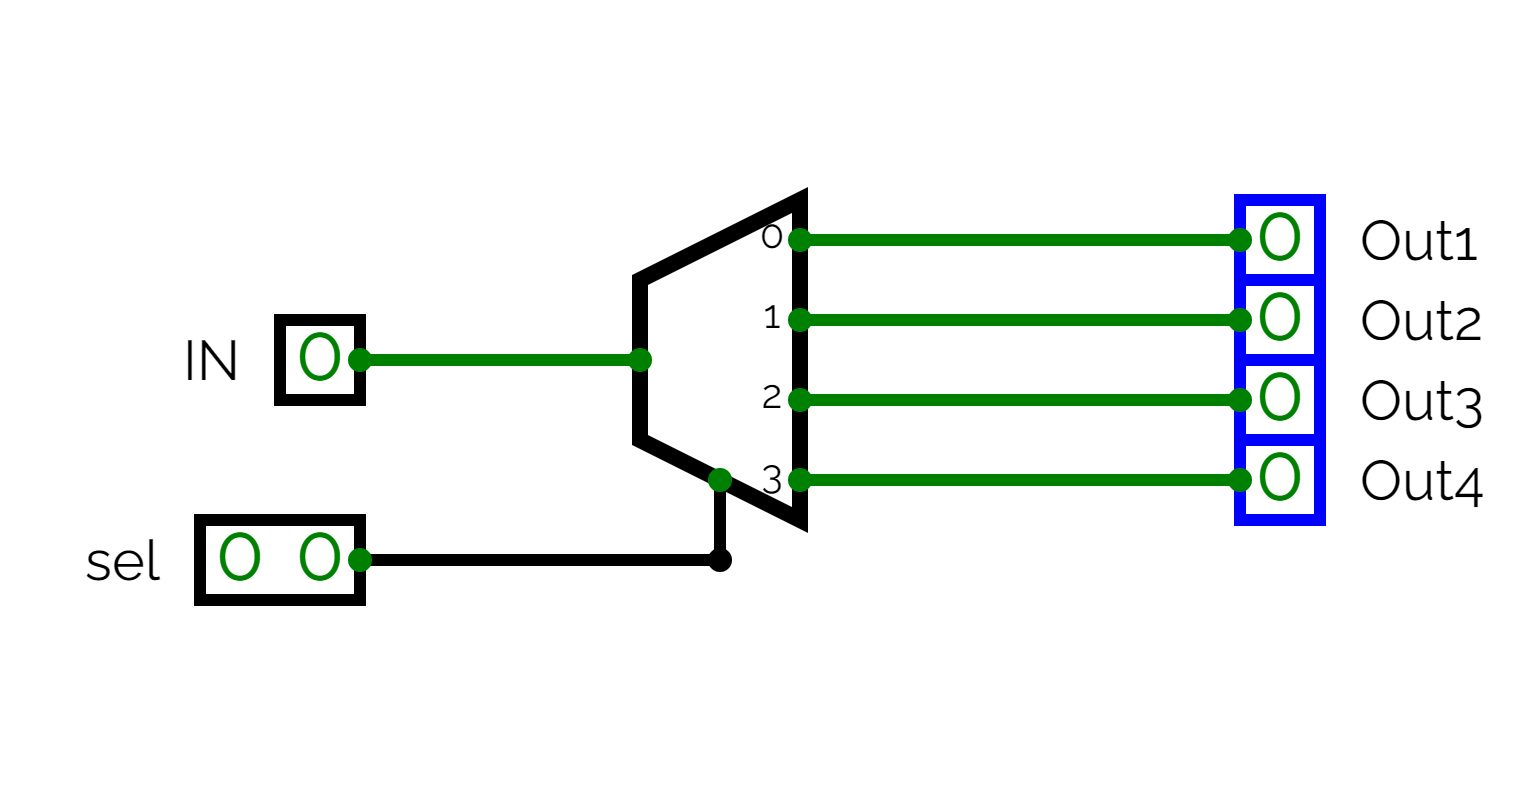
\includegraphics[width=1\textwidth]{CIRCUITOS/EXT/DMUX4WAY_ext.png}
	\caption{Circuito exterior de DMux4Way \cite{circuitverse}}
	\label{fig:dmux4way_ext}
\end{figure}
\subsection{Implementación HDL}
\begin{figure}[H]
	\centering
	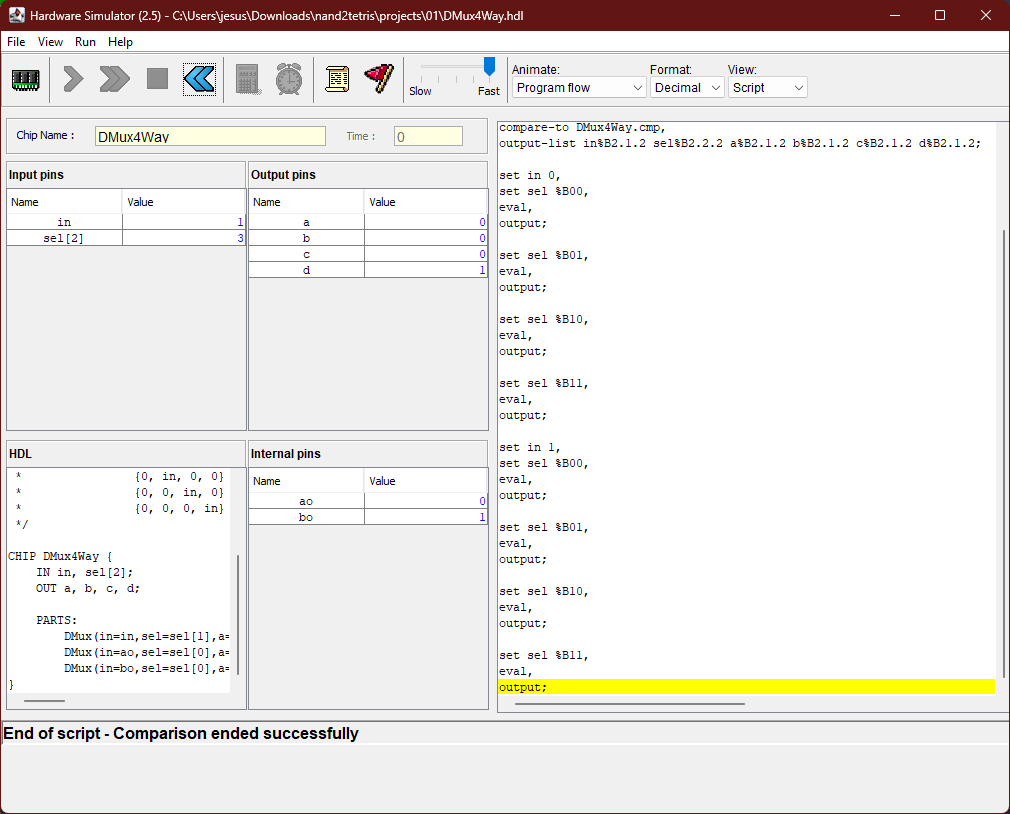
\includegraphics[width=0.75\linewidth]{CIRCUITOS//HDL/dmux4way.png}
	\caption{Test en Hardware Simulator de DMux4Way \cite{nand2tetris}}
	\label{fig:hdldmux4way}
\end{figure}
\subsubsection{Archivo HDL}
\begin{lstlisting}
	CHIP DMux4Way {
		IN in, sel[2];
		OUT a, b, c, d;

		PARTS:
		DMux(in=in,sel=sel[1],a=ao,b=bo);
		DMux(in=ao,sel=sel[0],a=a,b=b);
		DMux(in=bo,sel=sel[0],a=c,b=d);
	}
\end{lstlisting}
\newpage

%%%%%%%%%%%%%%%%%%%%%%%%%%%%%%%%%%%%%%%%%%%%%%%%%%%%%%%%%%%%%%%%%%%%%%%%%%
%%%%%%%%%%%%%%%%%%%%%%%%%%%%%%%%%%%%%%%%%%%%%%%%%%%%%%%%%%%%%%%%%%%%%%%%%%

\section{DMux8Way (DMuxi1o8b1)}
\subsection{Tabla de verdad y explicación del circuito}
Mismo concepto usado en \ref{dmux4label}, exceptuando que en vez de 4 outputs \ref{dmux4text}, se usan 8 outputs. \cite{nisan_nand2tetris_2005}

\begin{table}[H]
	\centering
	\caption{Tabla de verdad de DMUX8WAY}
	\label{tab:tab_dmux8way}
	\resizebox{0.8\columnwidth}{!}{%
		\begin{tabular}{@{}llllllllll@{}}
			\toprule
			\texttt{in} & \texttt{sel} & \texttt{a} & \texttt{b} & \texttt{c} & \texttt{d} & \texttt{e} & \texttt{f} & \texttt{g} & \texttt{h} \\ \midrule
			\texttt{0} & \texttt{000} & \texttt{0} & \texttt{0} & \texttt{0} & \texttt{0} & \texttt{0} & \texttt{0} & \texttt{0} & \texttt{0} \\
			\texttt{0} & \texttt{001} & \texttt{0} & \texttt{0} & \texttt{0} & \texttt{0} & \texttt{0} & \texttt{0} & \texttt{0} & \texttt{0} \\
			\texttt{0} & \texttt{010} & \texttt{0} & \texttt{0} & \texttt{0} & \texttt{0} & \texttt{0} & \texttt{0} & \texttt{0} & \texttt{0} \\
			\texttt{0} & \texttt{011} & \texttt{0} & \texttt{0} & \texttt{0} & \texttt{0} & \texttt{0} & \texttt{0} & \texttt{0} & \texttt{0} \\
			\texttt{0} & \texttt{100} & \texttt{0} & \texttt{0} & \texttt{0} & \texttt{0} & \texttt{0} & \texttt{0} & \texttt{0} & \texttt{0} \\
			\texttt{0} & \texttt{101} & \texttt{0} & \texttt{0} & \texttt{0} & \texttt{0} & \texttt{0} & \texttt{0} & \texttt{0} & \texttt{0} \\
			\texttt{0} & \texttt{110} & \texttt{0} & \texttt{0} & \texttt{0} & \texttt{0} & \texttt{0} & \texttt{0} & \texttt{0} & \texttt{0} \\
			\texttt{0} & \texttt{111} & \texttt{0} & \texttt{0} & \texttt{0} & \texttt{0} & \texttt{0} & \texttt{0} & \texttt{0} & \texttt{0} \\
			\texttt{1} & \texttt{000} & \texttt{1} & \texttt{0} & \texttt{0} & \texttt{0} & \texttt{0} & \texttt{0} & \texttt{0} & \texttt{0} \\
			\texttt{1} & \texttt{001} & \texttt{0} & \texttt{1} & \texttt{0} & \texttt{0} & \texttt{0} & \texttt{0} & \texttt{0} & \texttt{0} \\
			\texttt{1} & \texttt{010} & \texttt{0} & \texttt{0} & \texttt{1} & \texttt{0} & \texttt{0} & \texttt{0} & \texttt{0} & \texttt{0} \\
			\texttt{1} & \texttt{011} & \texttt{0} & \texttt{0} & \texttt{0} & \texttt{1} & \texttt{0} & \texttt{0} & \texttt{0} & \texttt{0} \\
			\texttt{1} & \texttt{100} & \texttt{0} & \texttt{0} & \texttt{0} & \texttt{0} & \texttt{1} & \texttt{0} & \texttt{0} & \texttt{0} \\
			\texttt{1} & \texttt{101} & \texttt{0} & \texttt{0} & \texttt{0} & \texttt{0} & \texttt{0} & \texttt{1} & \texttt{0} & \texttt{0} \\
			\texttt{1} & \texttt{110} & \texttt{0} & \texttt{0} & \texttt{0} & \texttt{0} & \texttt{0} & \texttt{0} & \texttt{1} & \texttt{0} \\
			\texttt{1} & \texttt{111} & \texttt{0} & \texttt{0} & \texttt{0} & \texttt{0} & \texttt{0} & \texttt{0} & \texttt{0} & \texttt{1} \\ \bottomrule
		\end{tabular}%
	}
\end{table}



\subsection{Esquema del circuito interior}
\begin{figure}[H]
	\centering
	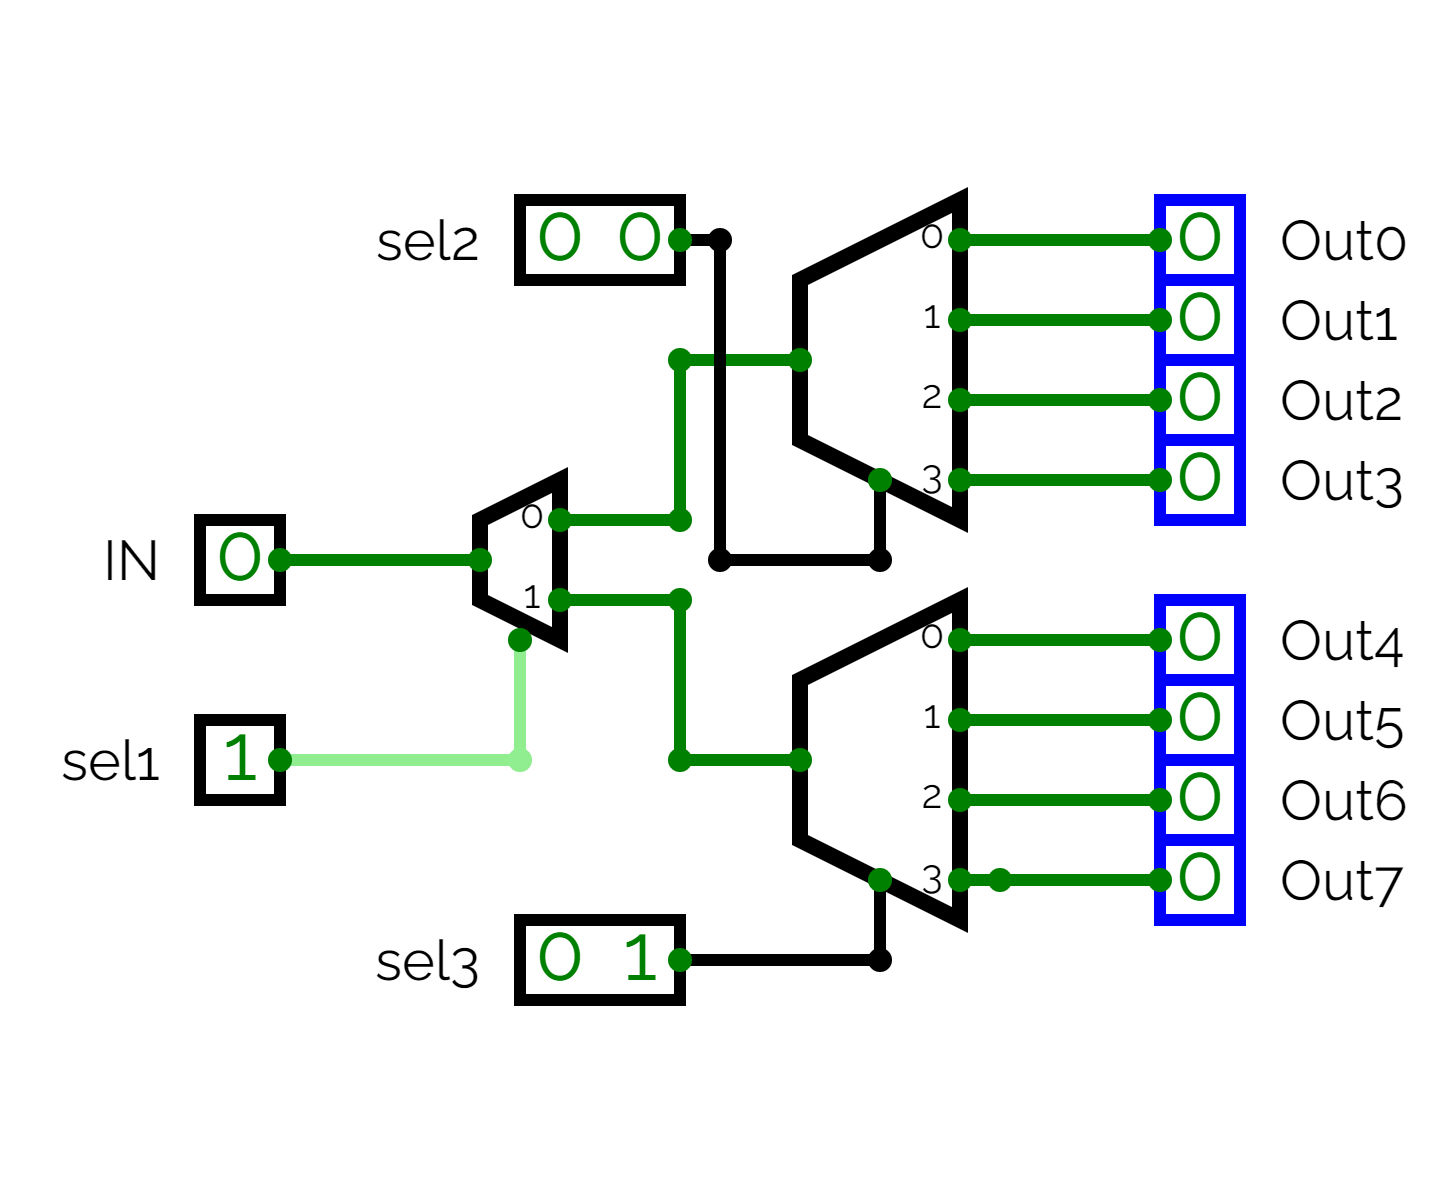
\includegraphics[width=1\textwidth]{CIRCUITOS/INT/Dmux8way_int.png}            \caption{Circuito interior de DMux8Way \cite{circuitverse}}
	\label{fig:dmux8way_int}
\end{figure}
\subsection{Esquema del circuito exterior}
\begin{figure}[H]
	\centering
	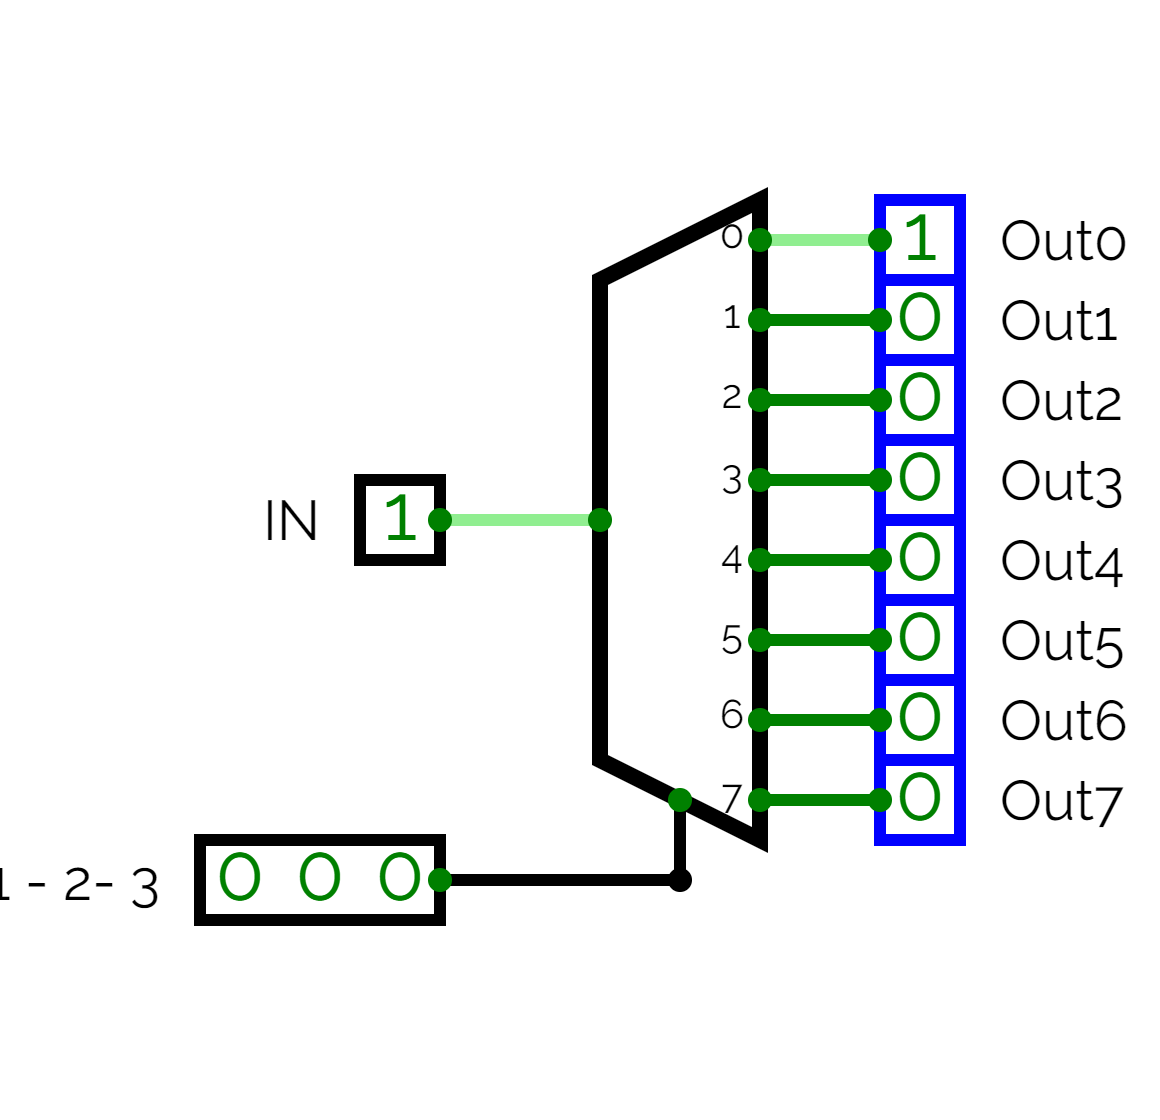
\includegraphics[width=1\textwidth]{CIRCUITOS/EXT/DMUX8WAY_ext.png}            \caption{Circuito exterior de DMux8Way \cite{circuitverse}}
	\label{fig:dmux8way_ext}
\end{figure}
\subsection{Implementación HDL}
\begin{figure}[H]
	\centering
	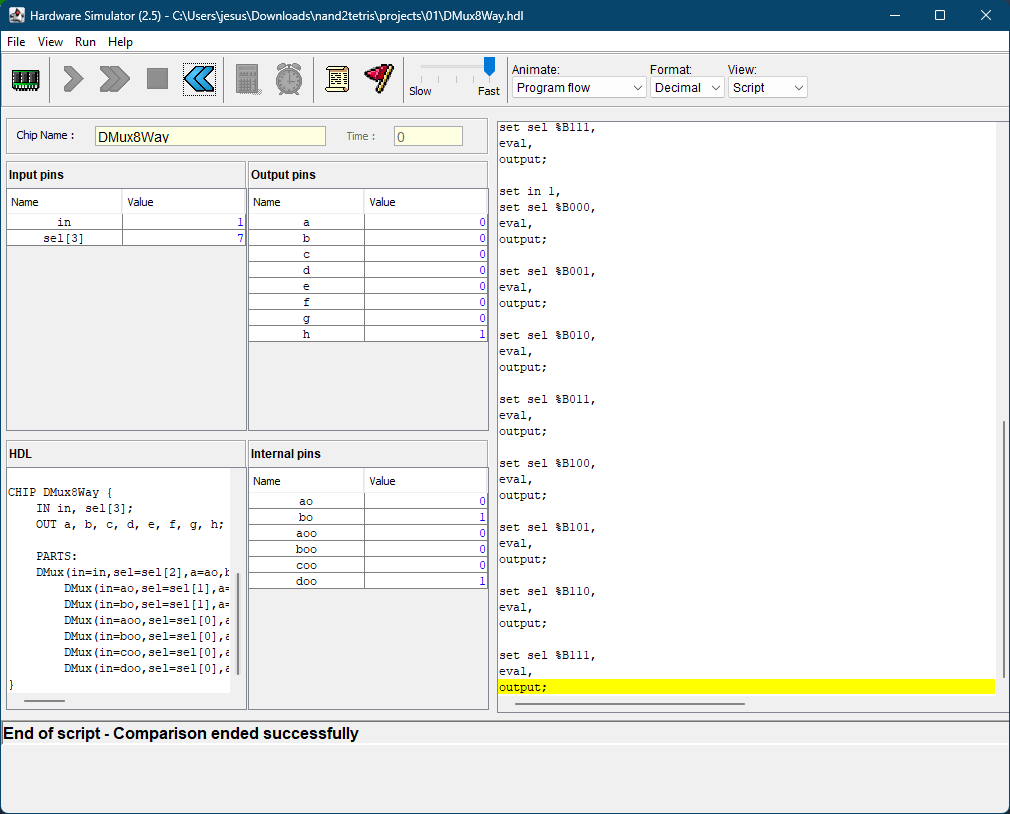
\includegraphics[width=0.75\linewidth]{CIRCUITOS//HDL/dmux8way.png}
	\caption{Test en Hardware Simulator de DMux8Way \cite{nand2tetris}}
	\label{fig:hdldmux8way}
\end{figure}
\subsubsection{Archivo HDL}
\begin{lstlisting}
	CHIP DMux8Way {
		IN in, sel[3];
		OUT a, b, c, d, e, f, g, h;

		PARTS:
		DMux(in=in,sel=sel[2],a=ao,b=bo);
		DMux(in=ao,sel=sel[1],a=aoo,b=boo);
		DMux(in=bo,sel=sel[1],a=coo,b=doo);
		DMux(in=aoo,sel=sel[0],a=a,b=b);
		DMux(in=boo,sel=sel[0],a=c,b=d);
		DMux(in=coo,sel=sel[0],a=e,b=f);
		DMux(in=doo,sel=sel[0],a=g,b=h);
	}
\end{lstlisting}
\newpage

%%%%%%%%%%%%%%%%%%%%%%%%%%%%%%%%%%%%%%%%%%%%%%%%%%%%%%%%%%%%%%%%%%%%%%%%%%
%%%%%%%%%%%%%%%%%%%%%%%%%%%%%%%%%%%%%%%%%%%%%%%%%%%%%%%%%%%%%%%%%%%%%%%%%%

\section{Mux4Way16 (Muxi4o1b16)} \label{mux4waytitle}
\subsection{Tabla de verdad y explicación del circuito}
Un multiplexador de \textit{M}-vías y \textit{N}-bits selecciona un bit de un input y lo transfiere a un output de 1 bit. La selección se produce mediante una colección de control bits de número \textit{k}, con fórmula $k = log_{2}m$. \cite{nisan_nand2tetris_2005} \label{mux4way}
\begin{table}[H]
	\centering
	\caption{Tabla de verdad de MUX4WAY16}
	\label{tab:tab_mux4way16}
	\resizebox{\textwidth}{!}{%
		\begin{tabular}{@{}llllll@{}}
			\toprule
			\texttt{a}                & \texttt{b}                & \texttt{c}                & \texttt{d}                & \texttt{sel} & \texttt{out}              \\ \midrule
			\texttt{0000000000000000} & \texttt{0000000000000000} & \texttt{0000000000000000} & \texttt{0000000000000000} & \texttt{00}  & \texttt{0000000000000000} \\
			\texttt{0000000000000000} & \texttt{0000000000000000} & \texttt{0000000000000000} & \texttt{0000000000000000} & \texttt{01}  & \texttt{0000000000000000} \\
			\texttt{0000000000000000} & \texttt{0000000000000000} & \texttt{0000000000000000} & \texttt{0000000000000000} & \texttt{10}  & \texttt{0000000000000000} \\ \midrule
			\texttt{0000000000000000} & \texttt{0000000000000000} & \texttt{0000000000000000} & \texttt{0000000000000000} & \texttt{11}  & \texttt{0000000000000000} \\
			\texttt{0001001000110100} & \texttt{1001100001110110} & \texttt{1010101010101010} & \texttt{0101010101010101} & \texttt{00}  & \texttt{0001001000110100} \\
			\texttt{0001001000110100} & \texttt{1001100001110110} & \texttt{1010101010101010} & \texttt{0101010101010101} & \texttt{01}  & \texttt{1001100001110110} \\
			\texttt{0001001000110100} & \texttt{1001100001110110} & \texttt{1010101010101010} & \texttt{0101010101010101} & \texttt{10}  & \texttt{1010101010101010} \\
			\texttt{0001001000110100} & \texttt{1001100001110110} & \texttt{1010101010101010} & \texttt{0101010101010101} & \texttt{11} & \textit{\texttt{0101010101010101}} \\ \bottomrule
		\end{tabular}%
	}
\end{table}

\subsection{Esquema del circuito interior}
\begin{figure}[H]
	\centering
	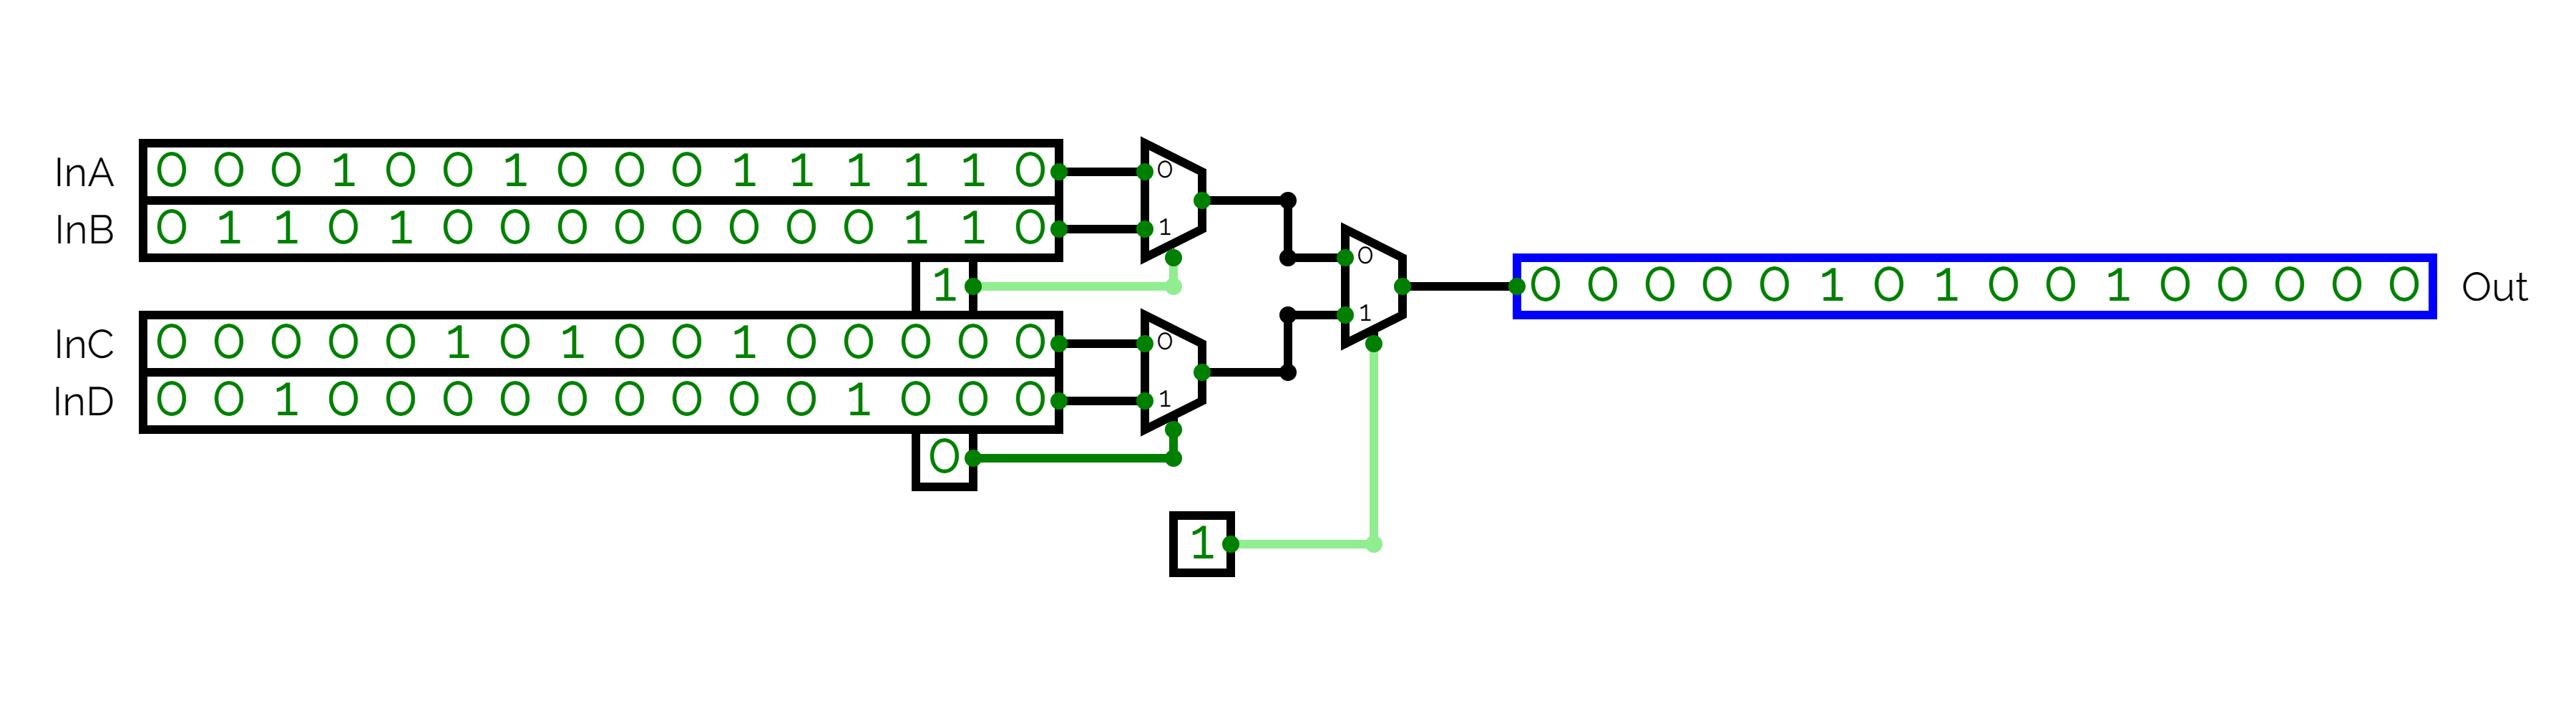
\includegraphics[width=1\textwidth]{CIRCUITOS/INT/Mux4Way16_int.png}            \caption{Circuito interior de Mux4Way16 \cite{circuitverse}}
	\label{fig:mux4way16_int}
\end{figure}
\subsection{Esquema del circuito exterior}
\begin{figure}[H]
	\centering
	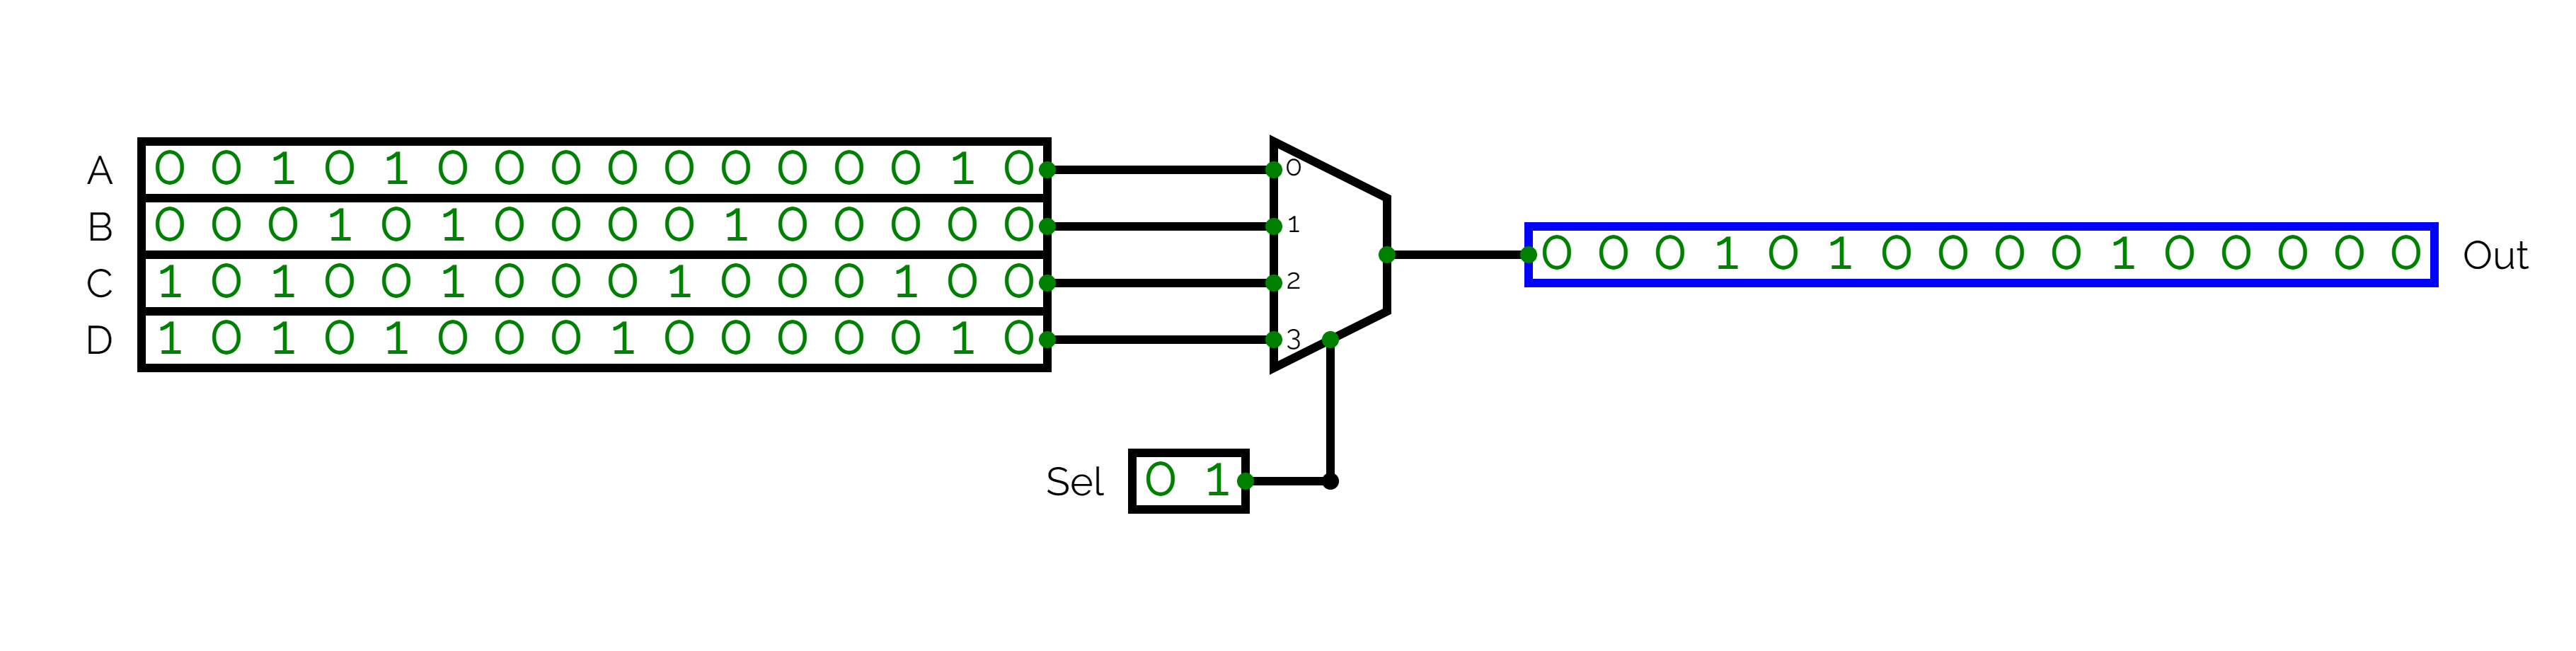
\includegraphics[width=1\textwidth]{CIRCUITOS/EXT/Mux4Way16_ext.png}            \caption{Circuito exterior de Mux4Way16 \cite{circuitverse}}
	\label{fig:mux4way16_ext}
\end{figure}
\subsection{Implementación HDL}
\begin{figure}[H]
	\centering
	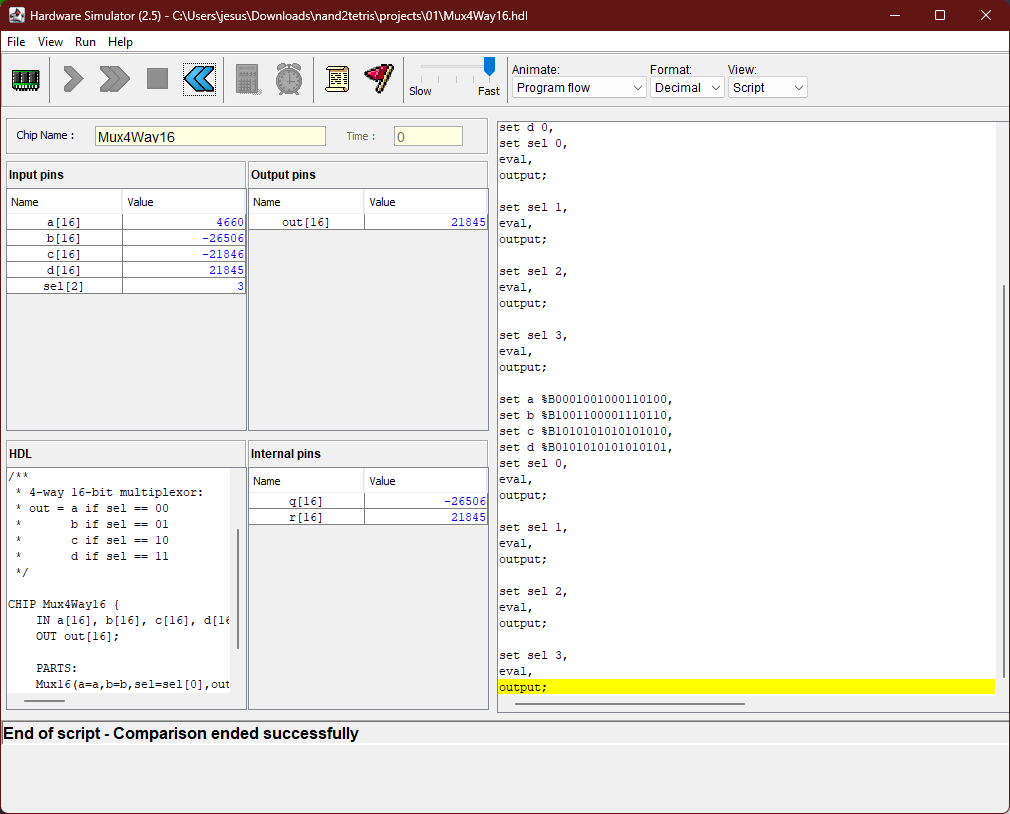
\includegraphics[width=0.75\linewidth]{mux4way16.png}
	\caption{Test en Hardware Simulator de Mux4Way16 \cite{nand2tetris}}
	\label{fig:hdlmux4way16}
\end{figure}
\subsubsection{Archivo HDL}
\begin{lstlisting}
	CHIP Mux4Way16 {
		IN a[16], b[16], c[16], d[16], sel[2];
		OUT out[16];

		PARTS:
		Mux16(a=a,b=b,sel=sel[0],out=q);
		Mux16(a=c,b=d,sel=sel[0],out=r);
		Mux16(a=q,b=r,sel=sel[1],out=out);
	}
\end{lstlisting}
\newpage

%%%%%%%%%%%%%%%%%%%%%%%%%%%%%%%%%%%%%%%%%%%%%%%%%%%%%%%%%%%%%%%%%%%%%%%%%%
%%%%%%%%%%%%%%%%%%%%%%%%%%%%%%%%%%%%%%%%%%%%%%%%%%%%%%%%%%%%%%%%%%%%%%%%%%

\section{Mux8Way16 (Muxi8o1b16)}
\subsection{Tabla de verdad y explicación del circuito}
Mismo circuito que se ha visto en: \ref{mux4waytitle}, con la descripción: \ref{mux4way}. En pocas palabras, es un multiplexador de 8 puertas, en lugar de 4. \cite{nisan_nand2tetris_2005}
\begin{table}[H]
	\centering
	\caption{Tabla de verdad de MUX8WAY16}
	\label{tab:tab_mux8way16}
	\resizebox{\columnwidth}{!}{%
		\begin{tabular}{@{}llllllllll@{}}
			\toprule
			\multicolumn{1}{c}{\texttt{a}} &
			\multicolumn{1}{c}{\texttt{b}} &
			\multicolumn{1}{c}{\texttt{c}} &
			\multicolumn{1}{c}{\texttt{d}} &
			\multicolumn{1}{c}{\texttt{e}} &
			\multicolumn{1}{c}{\texttt{f}} &
			\multicolumn{1}{c}{\texttt{g}} &
			\multicolumn{1}{c}{\texttt{h}} &
			\multicolumn{1}{c}{\texttt{sel}} &
			\multicolumn{1}{c}{\texttt{out}} \\ \midrule
			\texttt{0000000000000000} &
			\texttt{0000000000000000} &
			\texttt{0000000000000000} &
			\texttt{0000000000000000} &
			\texttt{0000000000000000} &
			\texttt{0000000000000000} &
			\texttt{0000000000000000} &
			\texttt{0000000000000000} &
			\texttt{000} &
			\texttt{0000000000000000} \\
			\texttt{0000000000000000} &
			\texttt{0000000000000000} &
			\texttt{0000000000000000} &
			\texttt{0000000000000000} &
			\texttt{0000000000000000} &
			\texttt{0000000000000000} &
			\texttt{0000000000000000} &
			\texttt{0000000000000000} &
			\texttt{001} &
			\texttt{0000000000000000} \\
			\texttt{0000000000000000} &
			\texttt{0000000000000000} &
			\texttt{0000000000000000} &
			\texttt{0000000000000000} &
			\texttt{0000000000000000} &
			\texttt{0000000000000000} &
			\texttt{0000000000000000} &
			\texttt{0000000000000000} &
			\texttt{010} &
			\texttt{0000000000000000} \\
			\texttt{0000000000000000} &
			\texttt{0000000000000000} &
			\texttt{0000000000000000} &
			\texttt{0000000000000000} &
			\texttt{0000000000000000} &
			\texttt{0000000000000000} &
			\texttt{0000000000000000} &
			\texttt{0000000000000000} &
			\texttt{011} &
			\texttt{0000000000000000} \\
			\texttt{0000000000000000} &
			\texttt{0000000000000000} &
			\texttt{0000000000000000} &
			\texttt{0000000000000000} &
			\texttt{0000000000000000} &
			\texttt{0000000000000000} &
			\texttt{0000000000000000} &
			\texttt{0000000000000000} &
			\texttt{100} &
			\texttt{0000000000000000} \\
			\texttt{0000000000000000} &
			\texttt{0000000000000000} &
			\texttt{0000000000000000} &
			\texttt{0000000000000000} &
			\texttt{0000000000000000} &
			\texttt{0000000000000000} &
			\texttt{0000000000000000} &
			\texttt{0000000000000000} &
			\texttt{101} &
			\texttt{0000000000000000} \\
			\texttt{0000000000000000} &
			\texttt{0000000000000000} &
			\texttt{0000000000000000} &
			\texttt{0000000000000000} &
			\texttt{0000000000000000} &
			\texttt{0000000000000000} &
			\texttt{0000000000000000} &
			\texttt{0000000000000000} &
			\texttt{110} &
			\texttt{0000000000000000} \\
			\texttt{0000000000000000} &
			\texttt{0000000000000000} &
			\texttt{0000000000000000} &
			\texttt{0000000000000000} &
			\texttt{0000000000000000} &
			\texttt{0000000000000000} &
			\texttt{0000000000000000} &
			\texttt{0000000000000000} &
			\texttt{111} &
			\texttt{0000000000000000} \\
			\texttt{0001001000110100} &
			\texttt{0010001101000101} &
			\texttt{0011010001010110} &
			\texttt{0100010101100111} &
			\texttt{0101011001111000} &
			\texttt{0110011110001001} &
			\texttt{0111100010011010} &
			\texttt{1000100110101011} &
			\texttt{000} &
			\texttt{0001001000110100} \\
			\texttt{0001001000110100} &
			\texttt{0010001101000101} &
			\texttt{0011010001010110} &
			\texttt{0100010101100111} &
			\texttt{0101011001111000} &
			\texttt{0110011110001001} &
			\texttt{0111100010011010} &
			\texttt{1000100110101011} &
			\texttt{001} &
			\texttt{0010001101000101} \\
			\texttt{0001001000110100} &
			\texttt{0010001101000101} &
			\texttt{0011010001010110} &
			\texttt{0100010101100111} &
			\texttt{0101011001111000} &
			\texttt{0110011110001001} &
			\texttt{0111100010011010} &
			\texttt{1000100110101011} &
			\texttt{010} &
			\texttt{0011010001010110} \\
			\texttt{0001001000110100} &
			\texttt{0010001101000101} &
			\texttt{0011010001010110} &
			\texttt{0100010101100111} &
			\texttt{0101011001111000} &
			\texttt{0110011110001001} &
			\texttt{0111100010011010} &
			\texttt{1000100110101011} &
			\texttt{011} &
			\texttt{0100010101100111} \\
			\texttt{0001001000110100} &
			\texttt{0010001101000101} &
			\texttt{0011010001010110} &
			\texttt{0100010101100111} &
			\texttt{0101011001111000} &
			\texttt{0110011110001001} &
			\texttt{0111100010011010} &
			\texttt{1000100110101011} &
			\texttt{100} &
			\texttt{0101011001111000} \\
			\texttt{0001001000110100} &
			\texttt{0010001101000101} &
			\texttt{0011010001010110} &
			\texttt{0100010101100111} &
			\texttt{0101011001111000} &
			\texttt{0110011110001001} &
			\texttt{0111100010011010} &
			\texttt{1000100110101011} &
			\texttt{101} &
			\texttt{0110011110001001} \\
			\texttt{0001001000110100} &
			\texttt{0010001101000101} &
			\texttt{0011010001010110} &
			\texttt{0100010101100111} &
			\texttt{0101011001111000} &
			\texttt{0110011110001001} &
			\texttt{0111100010011010} &
			\texttt{1000100110101011} &
			\texttt{110} &
			\texttt{0111100010011010} \\
			\texttt{0001001000110100} &
			\texttt{0010001101000101} &
			\texttt{0011010001010110} &
			\texttt{0100010101100111} &
			\texttt{0101011001111000} &
			\texttt{0110011110001001} &
			\texttt{0111100010011010} &
			\texttt{1000100110101011} &
			\texttt{111} &
			\texttt{1000100110101011} \\ \bottomrule
		\end{tabular}%
	}
\end{table}

\subsection{Esquema del circuito interior}
\begin{figure}[H]
	\centering
	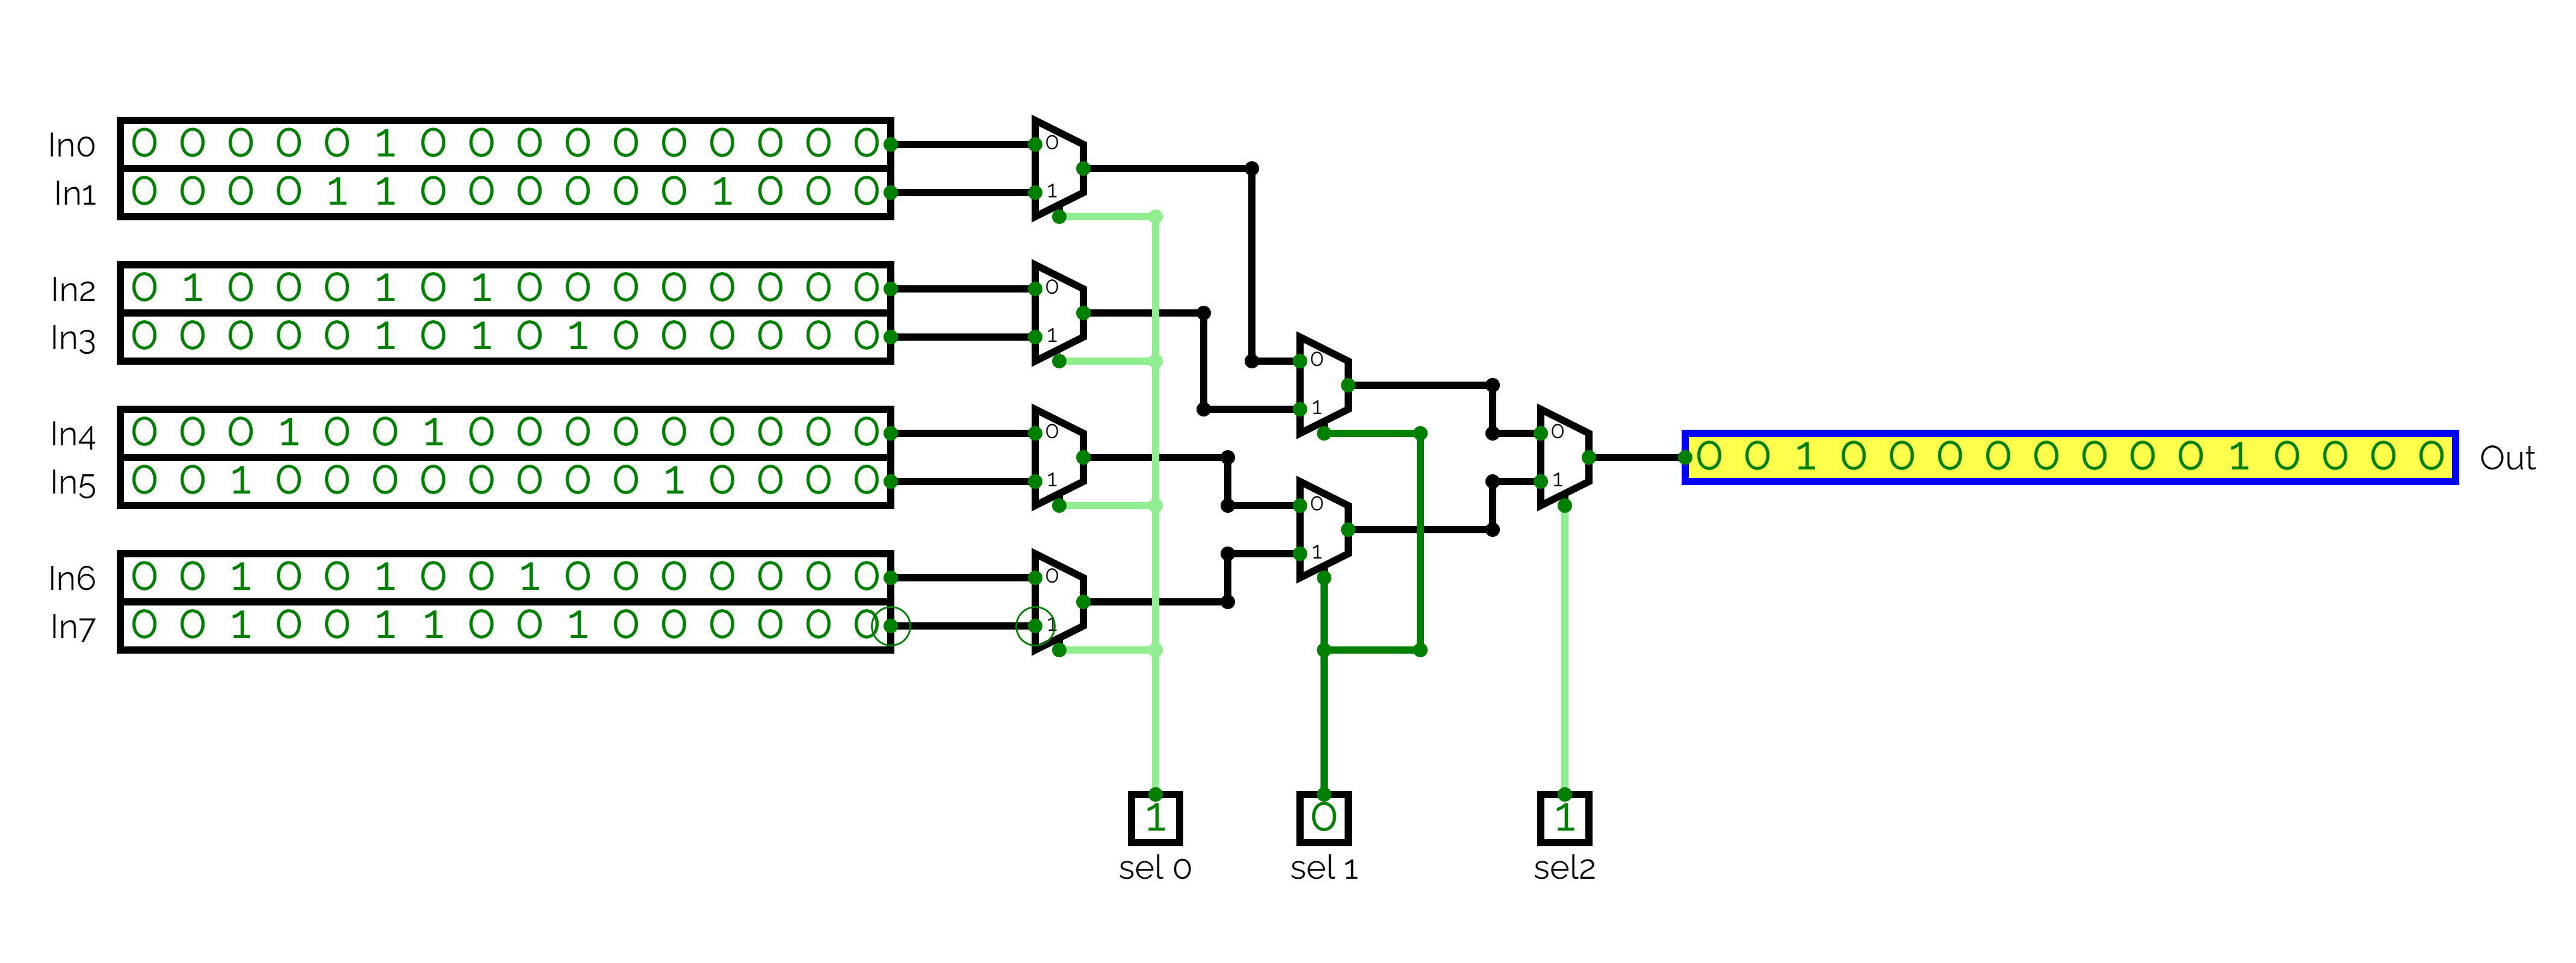
\includegraphics[width=1\textwidth]{CIRCUITOS/INT/Mux8Way16_int.png}            \caption{Circuito interior de Mux8Way16 \cite{circuitverse}}
	\label{fig:mux8way16_int}
\end{figure}
\subsection{Esquema del circuito exterior}
\begin{figure}[H]
	\centering
	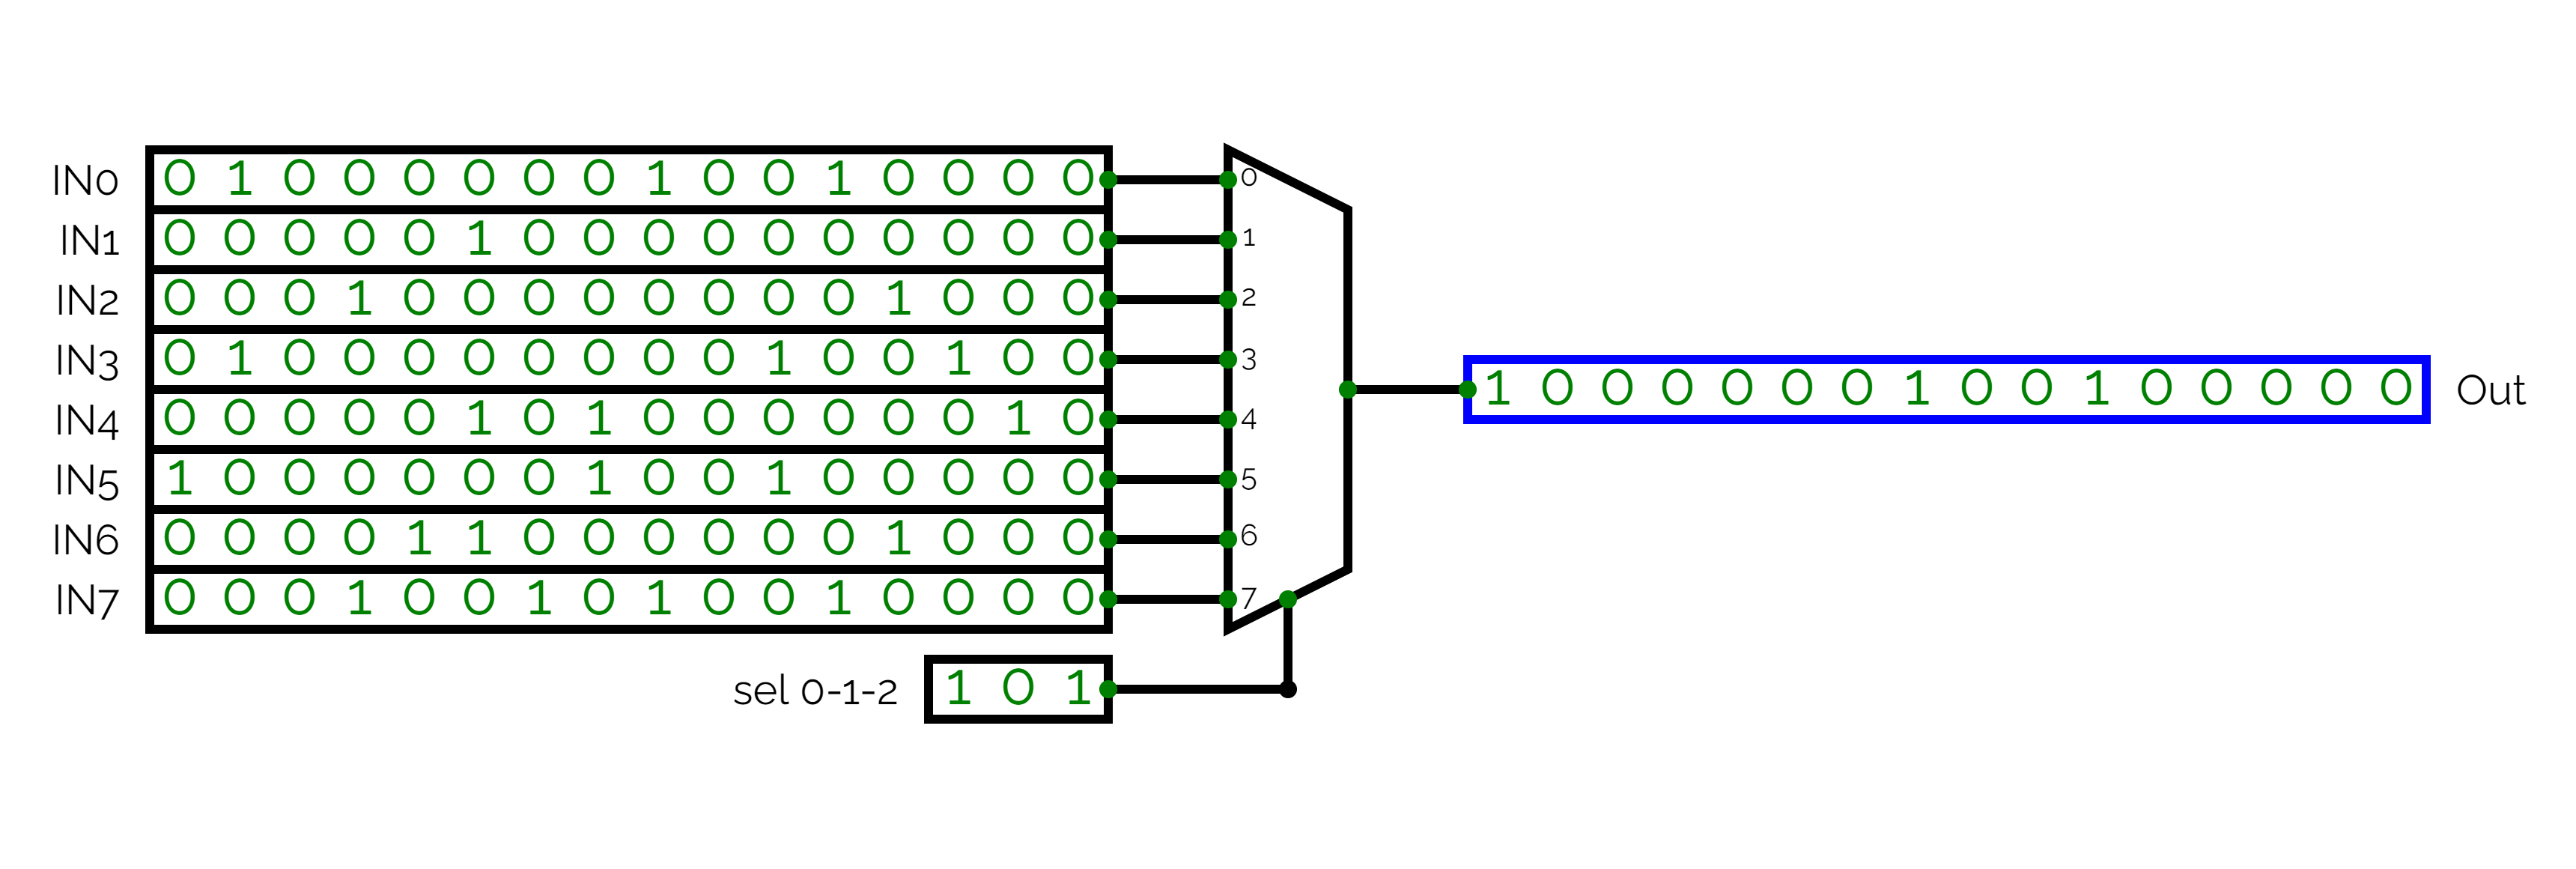
\includegraphics[width=1\textwidth]{CIRCUITOS/EXT/MUX8WAY16_ext.png}
	\caption{Circuito exterior de Mux8Way16 \cite{circuitverse}}
	\label{fig:mux8way16_ext}
\end{figure}
\subsection{Implementación HDL}
\begin{figure}[H]
	\centering
	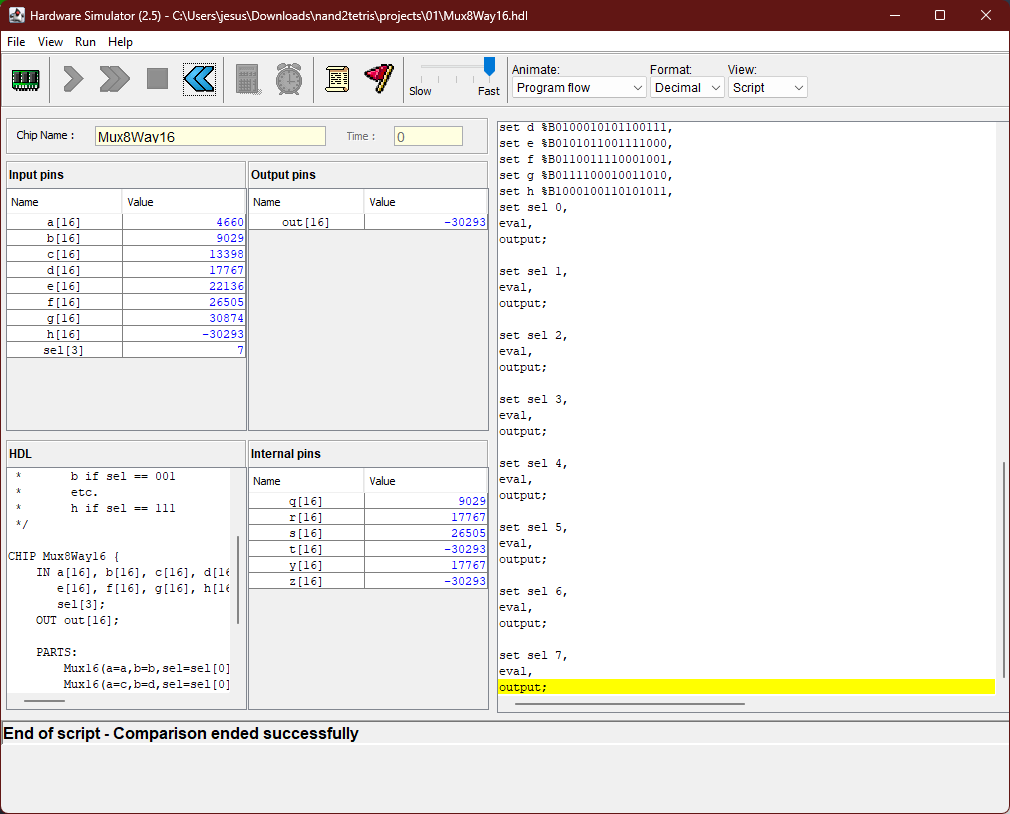
\includegraphics[width=0.75\linewidth]{CIRCUITOS//HDL/mux8way16_hdl.png}
	\caption{Test en Hardware Simulator de Mux8Way16 \cite{nand2tetris}}
	\label{fig:hdlmux8way16}
\end{figure}
\subsubsection{Archivo HDL}
\begin{lstlisting}
	CHIP Mux8Way16 {
		IN a[16], b[16], c[16], d[16],
		e[16], f[16], g[16], h[16],
		sel[3];
		OUT out[16];

		PARTS:
		Mux16(a=a,b=b,sel=sel[0],out=q);
		Mux16(a=c,b=d,sel=sel[0],out=r);
		Mux16(a=e,b=f,sel=sel[0],out=s);
		Mux16(a=g,b=h,sel=sel[0],out=t);
		Mux16(a=q,b=r,sel=sel[1],out=y);
		Mux16(a=s,b=t,sel=sel[1],out=z);
		Mux16(a=y,b=z,sel=sel[2],out=out);
	}
\end{lstlisting}
\newpage


%%%%%%%%%%%%%%%%%%%%%%%%%%%%%%%%%%%%%%%%%%%%%%%%%%%%%%%%%%%%%%%%%%%%%%%%%%
%%%%%%%%%%%%%%%%%%%%%%%%%%%%%%%%%%%%%%%%%%%%%%%%%%%%%%%%%%%%%%%%%%%%%%%%%%

\section{Or8Way (Ori8o1b1)}
\subsection{Tabla de verdad y explicación del circuito}
Un Or de \textit{N}-puertas produce en el output un 1 cuando \textit{al menos} uno de los inputs es 1, y 0 en caso contrario. \cite{nisan_nand2tetris_2005}
\begin{table}[H]
	\centering
	\caption{Tabla de verdad de Or8Way}
	\label{tab:tab_Or8way}
	\resizebox{0.25\textwidth}{!}{%
		\begin{tabular}{@{}ll@{}}
			\toprule
			\texttt{in}       & \texttt{out} \\ \midrule
			\texttt{00000000} & \texttt{0}   \\
			\texttt{11111111} & \texttt{1}   \\
			\texttt{00010000} & \texttt{1}   \\
			\texttt{00000001} & \texttt{1}   \\
			\texttt{00100110} & \texttt{1}   \\ \bottomrule
		\end{tabular}%
	}
\end{table}

\subsection{Esquema del circuito interior}
\begin{figure}[H]
	\centering
	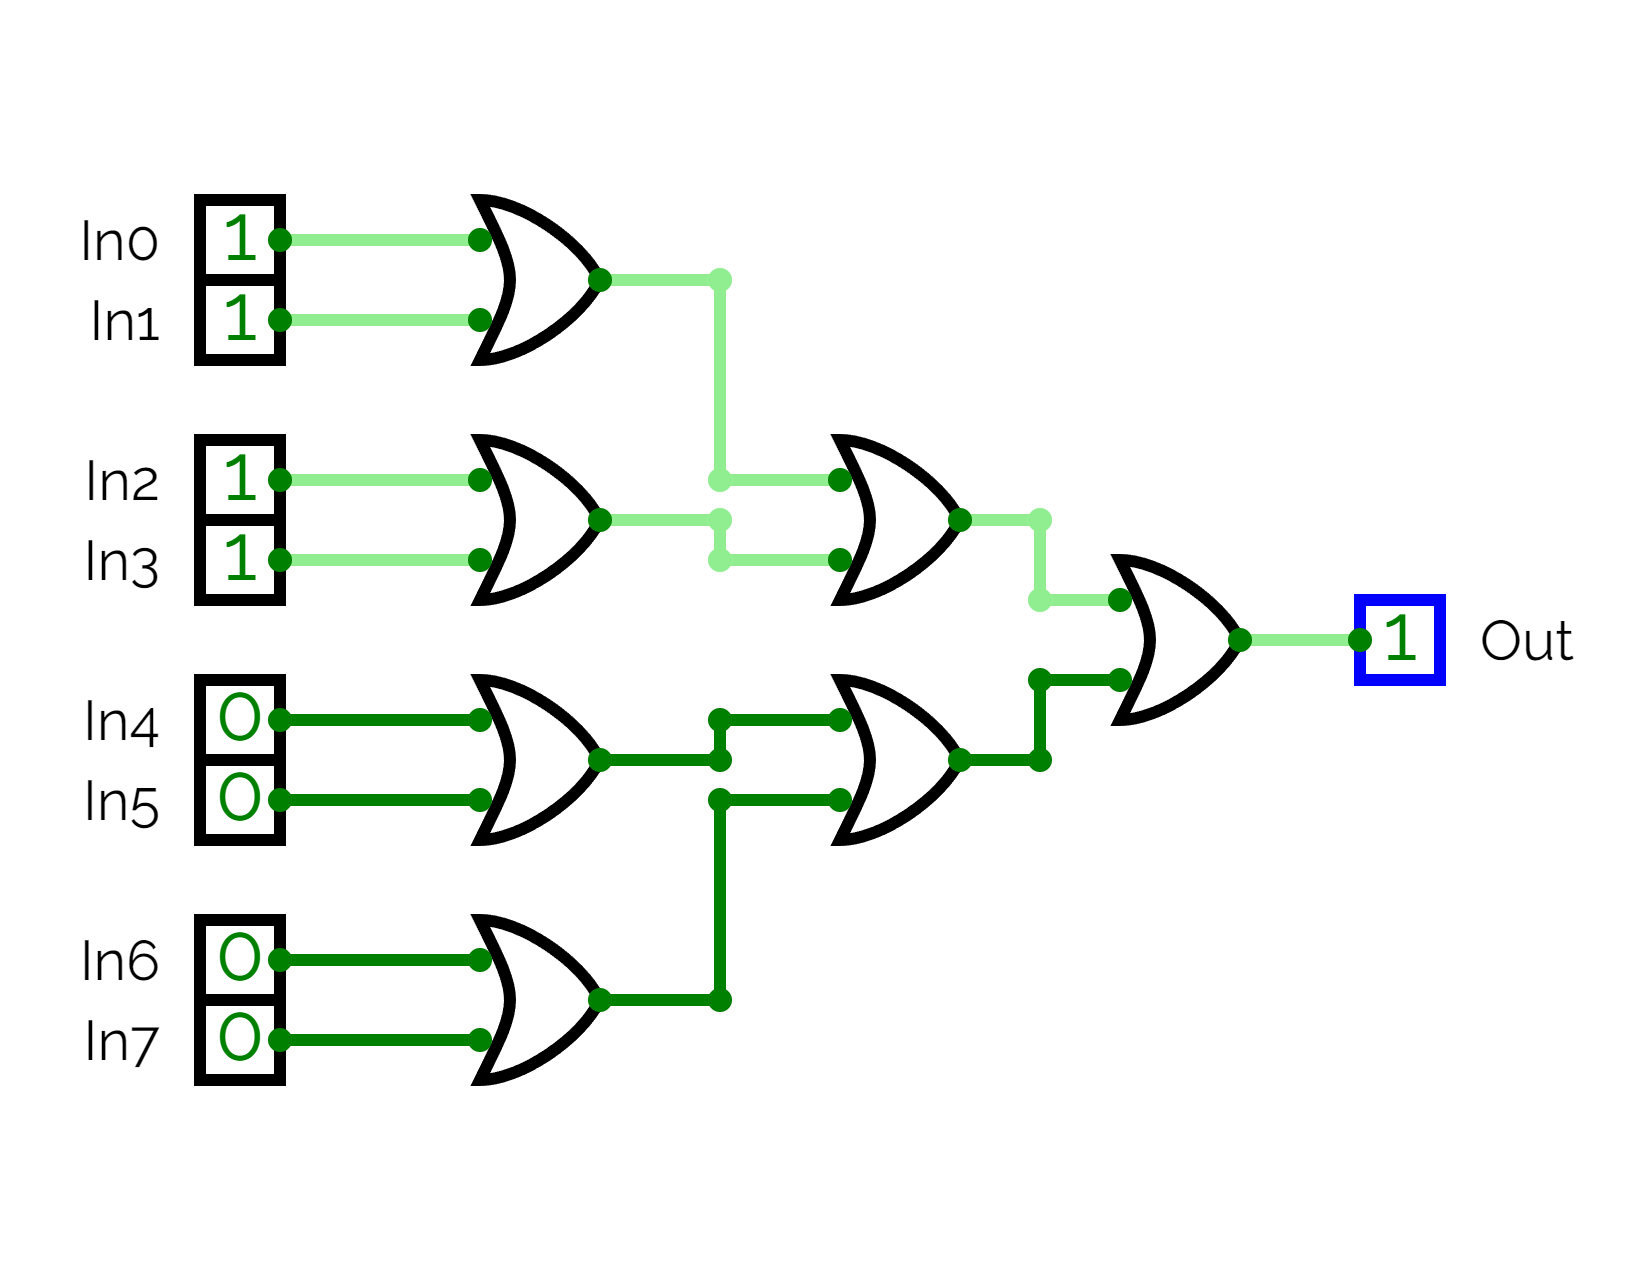
\includegraphics[width=1\textwidth]{CIRCUITOS/INT/OR8Way_int.png}            \caption{Circuito interior de Or8Way \cite{circuitverse}}
	\label{fig:or8way_int}
\end{figure}
\subsection{Esquema del circuito exterior}
\begin{figure}[H]
	\centering
	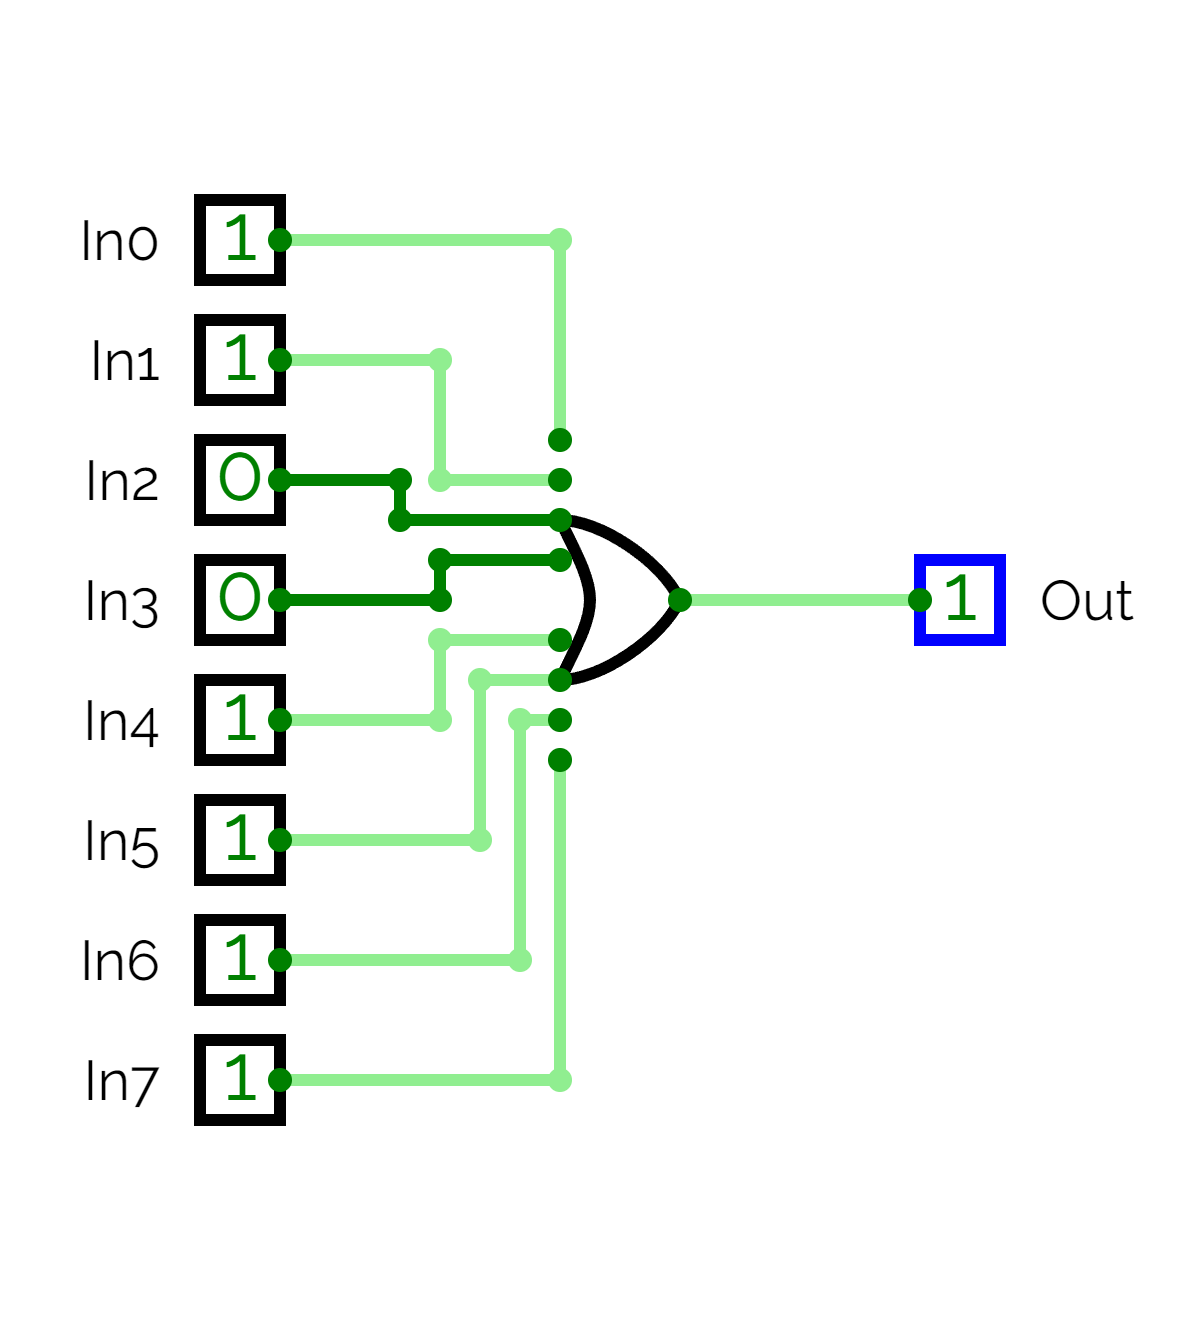
\includegraphics[width=0.8\textwidth]{CIRCUITOS/EXT/Or8Way_ext.png}            \caption{Circuito exterior de Or8Way \cite{circuitverse}}
	\label{fig:or8way_ext}
\end{figure}
\subsection{Implementación HDL}
\begin{figure}[H]
	\centering
	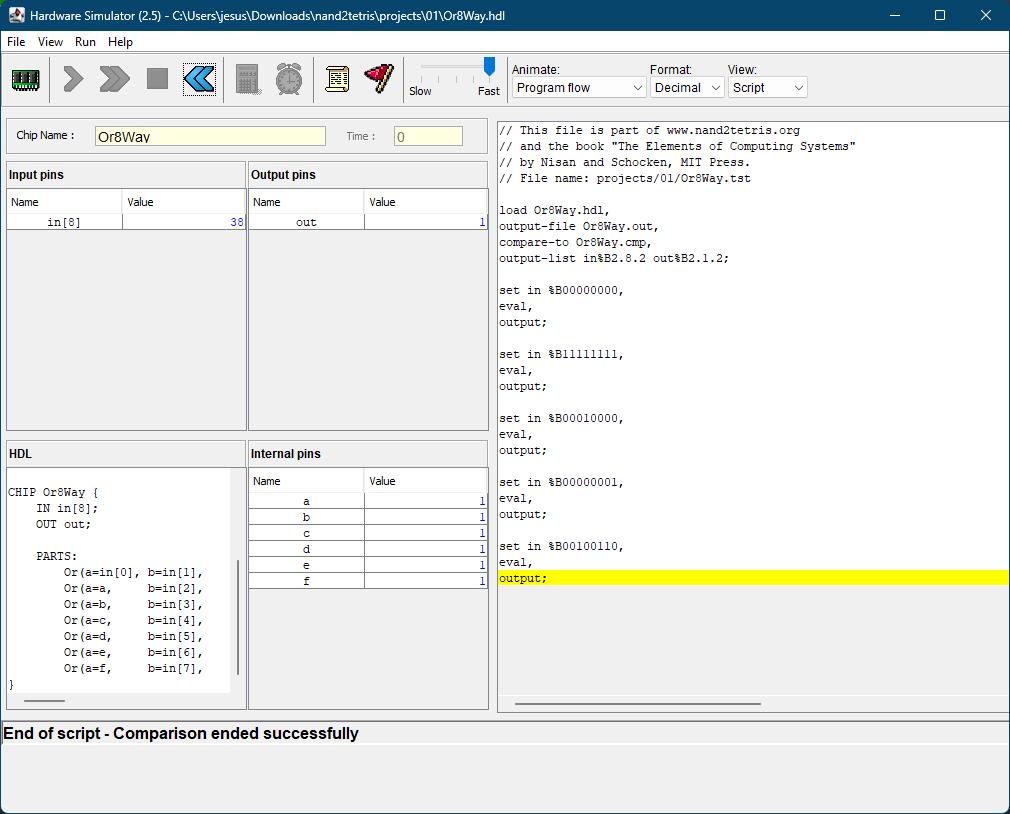
\includegraphics[width=0.75\linewidth]{CIRCUITOS//HDL/or8way.png}
	\caption{Test en Hardware Simulator de Or8Way \cite{nand2tetris}}
	\label{fig:hdlor8way}
\end{figure}
\subsubsection{Archivo HDL}
\begin{lstlisting}
	CHIP Or8Way {
		IN in[8];
		OUT out;

		PARTS:
		Or(a=in[0], b=in[1],     out=a);
		Or(a=a,     b=in[2],     out=b);
		Or(a=b,     b=in[3],     out=c);
		Or(a=c,     b=in[4],     out=d);
		Or(a=d,     b=in[5],     out=e);
		Or(a=e,     b=in[6],     out=f);
		Or(a=f,     b=in[7],     out=out);
	}
\end{lstlisting}
\newpage
\end{comment}
\part{Aritmética Booleana}
\section{HalfAdder}
\hrule
\vspace{0.5cm}
\subsection{Tabla de verdad y explicación del circuito}
El Half-Adder hace la operación de adición de dos números binarios (dos bits) y da dos outputs, la suma de estos y el acarreo.
La suma se produce con dos puertas, un XOR, que lleva la suma y produce un 1 cuando A o B es 1, pero no ambos. Y una AND que produce 1 solamente cuando A y B son 1.
\begin{table}[H]
	\centering
	\caption{Tabla de verdad de HalfAdder}
	\label{tab:halfadder}
	\begin{tblr}{
			width = \linewidth,
			colspec = {Q[87]Q[87]Q[315]Q[350]},
			hline{1,6} = {-}{0.08em},
			hline{2} = {-}{0.05em},
		}
		\texttt{A} & \texttt{B} & \texttt{Sum (S)} & \texttt{Carry (C)} \\
		\texttt{0} & \texttt{0} & \texttt{0}       & \texttt{0}         \\
		\texttt{0} & \texttt{1} & \texttt{1}       & \texttt{0}         \\
		\texttt{1} & \texttt{0} & \texttt{1}       & \texttt{0}         \\
		\texttt{1} & \texttt{1} & \texttt{0}       & \texttt{1}
	\end{tblr}
\end{table}

\subsection{Esquema del circuito exterior y exterior}
\begin{figure}[H]
	\centering
	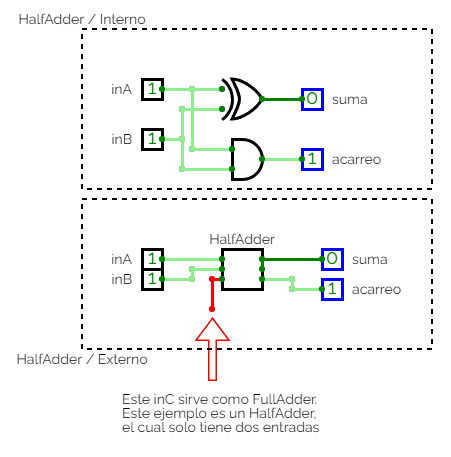
\includegraphics[width=0.75\linewidth]{ALU/HalfAdder.png}
	\caption{Esquema interior/exterior del circuito HalfAdder}
	\label{fig:h_adder}
\end{figure}
\subsection{Implementación HDL}
\begin{figure}[H]
	\centering
	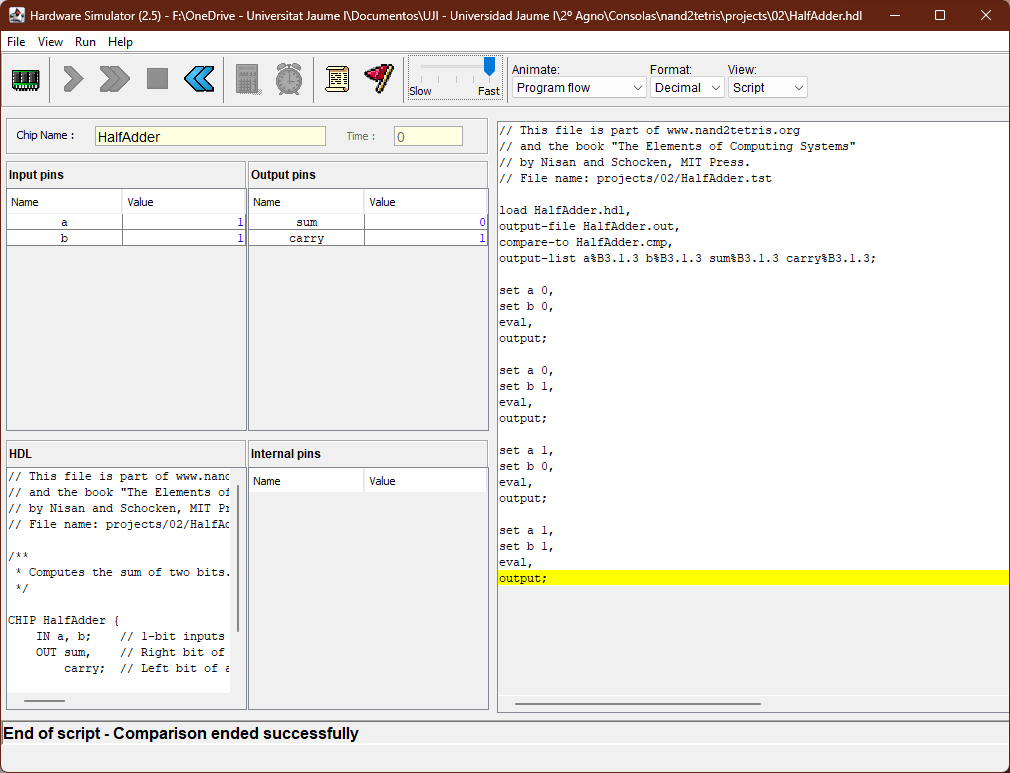
\includegraphics[width=0.75\linewidth]{ALU/halfadder_hw.png}
	\caption{Test de HalfAdder}
	\label{fig:enter-label}
\end{figure}
\subsubsection{Archivo .HDL}
\begin{lstlisting}
	CHIP HalfAdder {
		IN a, b;    // 1-bit inputs
		OUT sum,    // Right bit of a + b
		carry;  // Left bit of a + b

		PARTS:
		Xor(a=a,b=b,out=sum);
		And(a=a,b=b,out=carry);
	}
\end{lstlisting}
\newpage
\subsubsection{Archivo .TST}
\begin{lstlisting}
	load HalfAdder.hdl,
	output-file HalfAdder.out,
	compare-to HalfAdder.cmp,
	output-list a%B3.1.3 b%B3.1.3 sum%B3.1.3 carry%B3.1.3;

	set a 0,
	set b 0,
	eval,
	output;

	set a 0,
	set b 1,
	eval,
	output;

	set a 1,
	set b 0,
	eval,
	output;

	set a 1,
	set b 1,
	eval,
	output;

\end{lstlisting}
\subsubsection{Archivo .CMP}
\begin{lstlisting}
	|   a   |   b   |  sum  | carry |
	|   0   |   0   |   0   |   0   |
	|   0   |   1   |   1   |   0   |
	|   1   |   0   |   1   |   0   |
	|   1   |   1   |   0   |   1   |
\end{lstlisting}
\newpage
%%%%%%%%%%%%%%%%%%%%%%%%%%%%%%%%%%%%%%%%%%%%%%%%%%%%%%%%%%%%%%%%%%%%%%%%%%
%%%%%%%%%%%%%%%%%%%%%%%%%%%%%%%%%%%%%%%%%%%%%%%%%%%%%%%%%%%%%%%%%%%%%%%%%%
\section{FullAdder}
\subsection{Tabla de verdad y explicación del circuito}
EL FullAdder actúa como un Half exceptuando que contiene 3 inputs (3 bits). Su circuito se compone de 2 HalfAdders y se selecciona si contiene acarreo con una puerta OR.
\begin{table}[H]
	\centering
	\caption{Tabla de verdad de Full Adder}
	\label{tab:fulladder}
	\begin{tblr}{
			width = \linewidth,
			colspec = {Q[77]Q[77]Q[133]Q[279]Q[287]},
			hline{1,10} = {-}{0.08em},
			hline{2,7} = {-}{},
		}
		A & B & Cin & Sum (S) & Cout (C) \\
		0 & 0 & 0   & 0       & 0        \\
		0 & 0 & 1   & 1       & 0        \\
		0 & 1 & 0   & 1       & 0        \\
		0 & 1 & 1   & 0       & 1        \\
		1 & 0 & 0   & 1       & 0        \\
		1 & 0 & 1   & 0       & 1        \\
		1 & 1 & 0   & 0       & 1        \\
		1 & 1 & 1   & 1       & 1
	\end{tblr}
\end{table}

\subsection{Esquema del circuito exterior y exterior}
\begin{figure}[H]
	\centering
	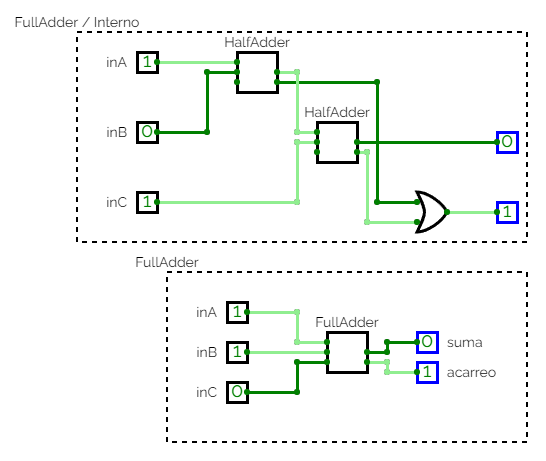
\includegraphics[width=0.75\linewidth]{ALU/FullAdder.png}
	\caption{Esquema interior/exterior del circuito FullAdder}
	\label{fig:f_adder}
\end{figure}
\subsection{Implementación HDL}
\begin{figure}[H]
	\centering
	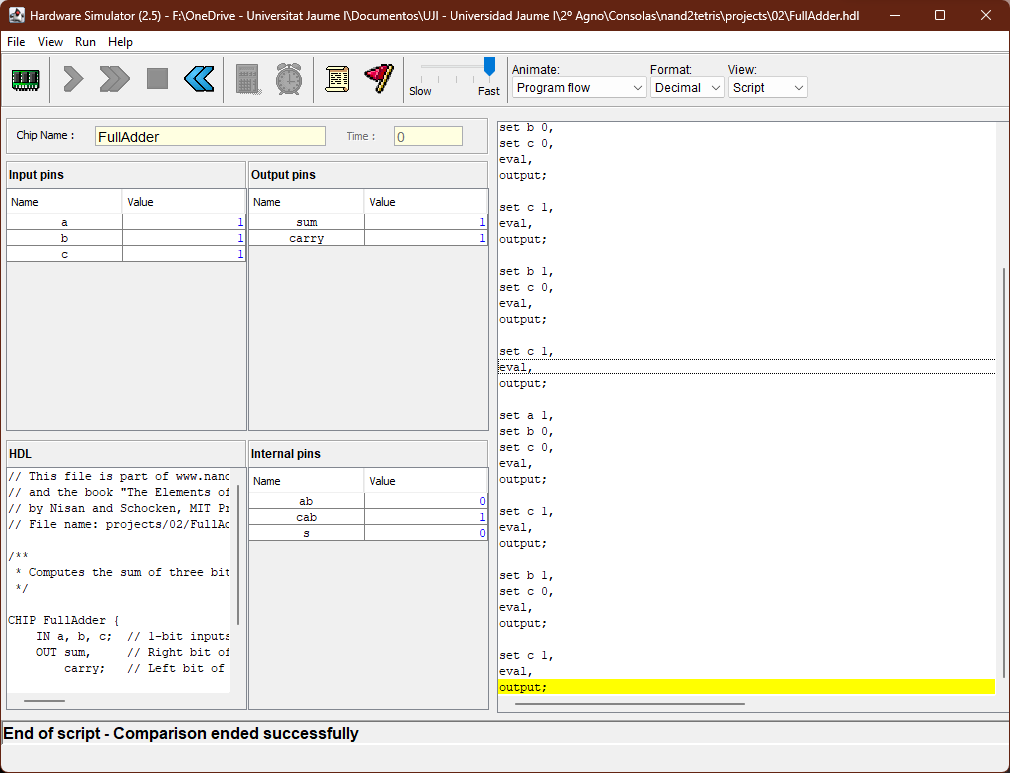
\includegraphics[width=0.75\linewidth]{ALU/fulladder_hw.png}
	\caption{Test de FullAdder}
	\label{fig:enter-label}
\end{figure}
\subsubsection{Archivo .HDL}
\begin{lstlisting}
	CHIP FullAdder {
		IN a, b, c;  // 1-bit inputs
		OUT sum,     // Right bit of a + b + c
		carry;   // Left bit of a + b + c

		PARTS:
		HalfAdder(a=a,b=b,sum=ab,carry=cab);
		HalfAdder(a=c,b=ab,sum=sum,carry=s);
		Or(a=cab,b=s,out=carry);
	}
\end{lstlisting}
\subsubsection{Archivo .TST}
\begin{lstlisting}
	load FullAdder.hdl,
	output-file FullAdder.out,
	compare-to FullAdder.cmp,
	output-list a%B3.1.3 b%B3.1.3 c%B3.1.3 sum%B3.1.3 carry%B3.1.3;

	set a 0,
	set b 0,
	set c 0,
	eval,
	output;

	set c 1,
	eval,
	output;

	set b 1,
	set c 0,
	eval,
	output;

	set c 1,
	eval,
	output;

	set a 1,
	set b 0,
	set c 0,
	eval,
	output;

	set c 1,
	eval,
	output;

	set b 1,
	set c 0,
	eval,
	output;

	set c 1,
	eval,
	output;

\end{lstlisting}
\subsubsection{Archivo .CMP}
\begin{lstlisting}
	|   a   |   b   |   c   |  sum  | carry |
	|   0   |   0   |   0   |   0   |   0   |
	|   0   |   0   |   1   |   1   |   0   |
	|   0   |   1   |   0   |   1   |   0   |
	|   0   |   1   |   1   |   0   |   1   |
	|   1   |   0   |   0   |   1   |   0   |
	|   1   |   0   |   1   |   0   |   1   |
	|   1   |   1   |   0   |   0   |   1   |
	|   1   |   1   |   1   |   1   |   1   |
\end{lstlisting}
\newpage
%%%%%%%%%%%%%%%%%%%%%%%%%%%%%%%%%%%%%%%%%%%%%%%%%%%%%%%%%%%%%%%%%%%%%%%%%%
%%%%%%%%%%%%%%%%%%%%%%%%%%%%%%%%%%%%%%%%%%%%%%%%%%%%%%%%%%%%%%%%%%%%%%%%%%
\section{Add16}
\subsection{Tabla de verdad y explicación del circuito}
El Add16 actúa como un adder, cuyo propósito es hacer la operación de suma con dos inputs de 16 bits. Funciona conectando varios FullAdders.
% \usepackage{color}
% \usepackage{tabularray}
\begin{table}[H]
	\centering
	\caption{Tabla de verdad de Add16}
	\label{tab:fulladder}
	\begin{tblr}{
			width = \linewidth,
			colspec = {Q[133]Q[135]Q[135]Q[196]Q[96]Q[217]},
			cells = {c, font=\ttfamily}, % Set font to monospaced (typewriter)
			vlines,
			hline{1,10} = {-}{0.08em},
			hline{2} = {-}{},
		}
		Inputs  & $A$ & $B$ & $C_{in}$ & Sum & $C_{out}$ \\
		Input 1 & 0   & 0   & 0      & 0   & 0       \\
		Input 2 & 0   & 0   & 1      & 1   & 0       \\
		Input 3 & 0   & 1   & 0      & 1   & 0       \\
		Input 4 & 0   & 1   & 1      & 0   & 1       \\
		Input 5 & 1   & 0   & 0      & 1   & 0       \\
		Input 6 & 1   & 0   & 1      & 0   & 1       \\
		Input 7 & 1   & 1   & 0      & 0   & 1       \\
		Input 8 & 1   & 1   & 1      & 1   & 1
	\end{tblr}
\end{table}
\subsection{Esquema del circuito exterior y exterior}
\subsubsection{Exterior}
\begin{figure}[H]
	\centering
	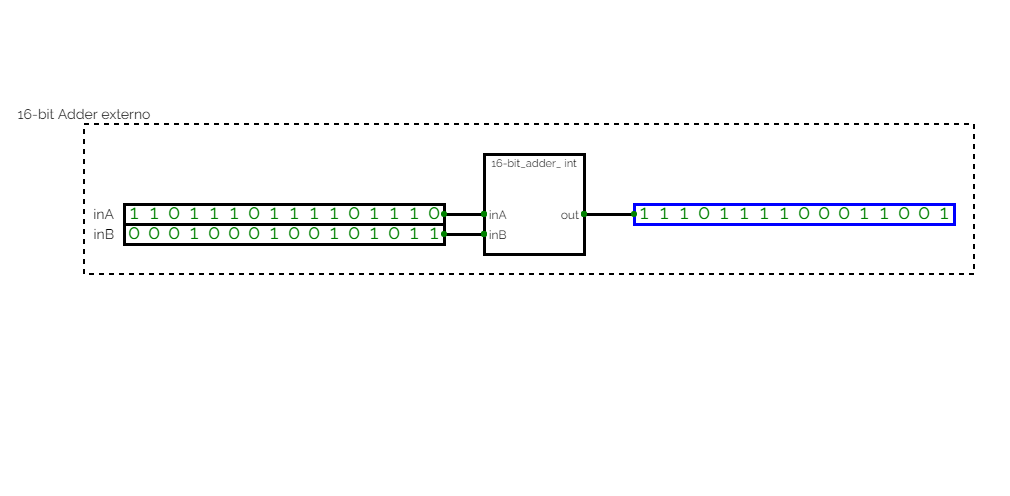
\includegraphics[width=0.75\linewidth]{ALU/16-bit_adder_ext.png}
	\caption{Esquema exterior del circuito Add16}
	\label{fig:add16}
\end{figure}
\subsubsection{Interior}
\begin{figure}[H]
	\centering
	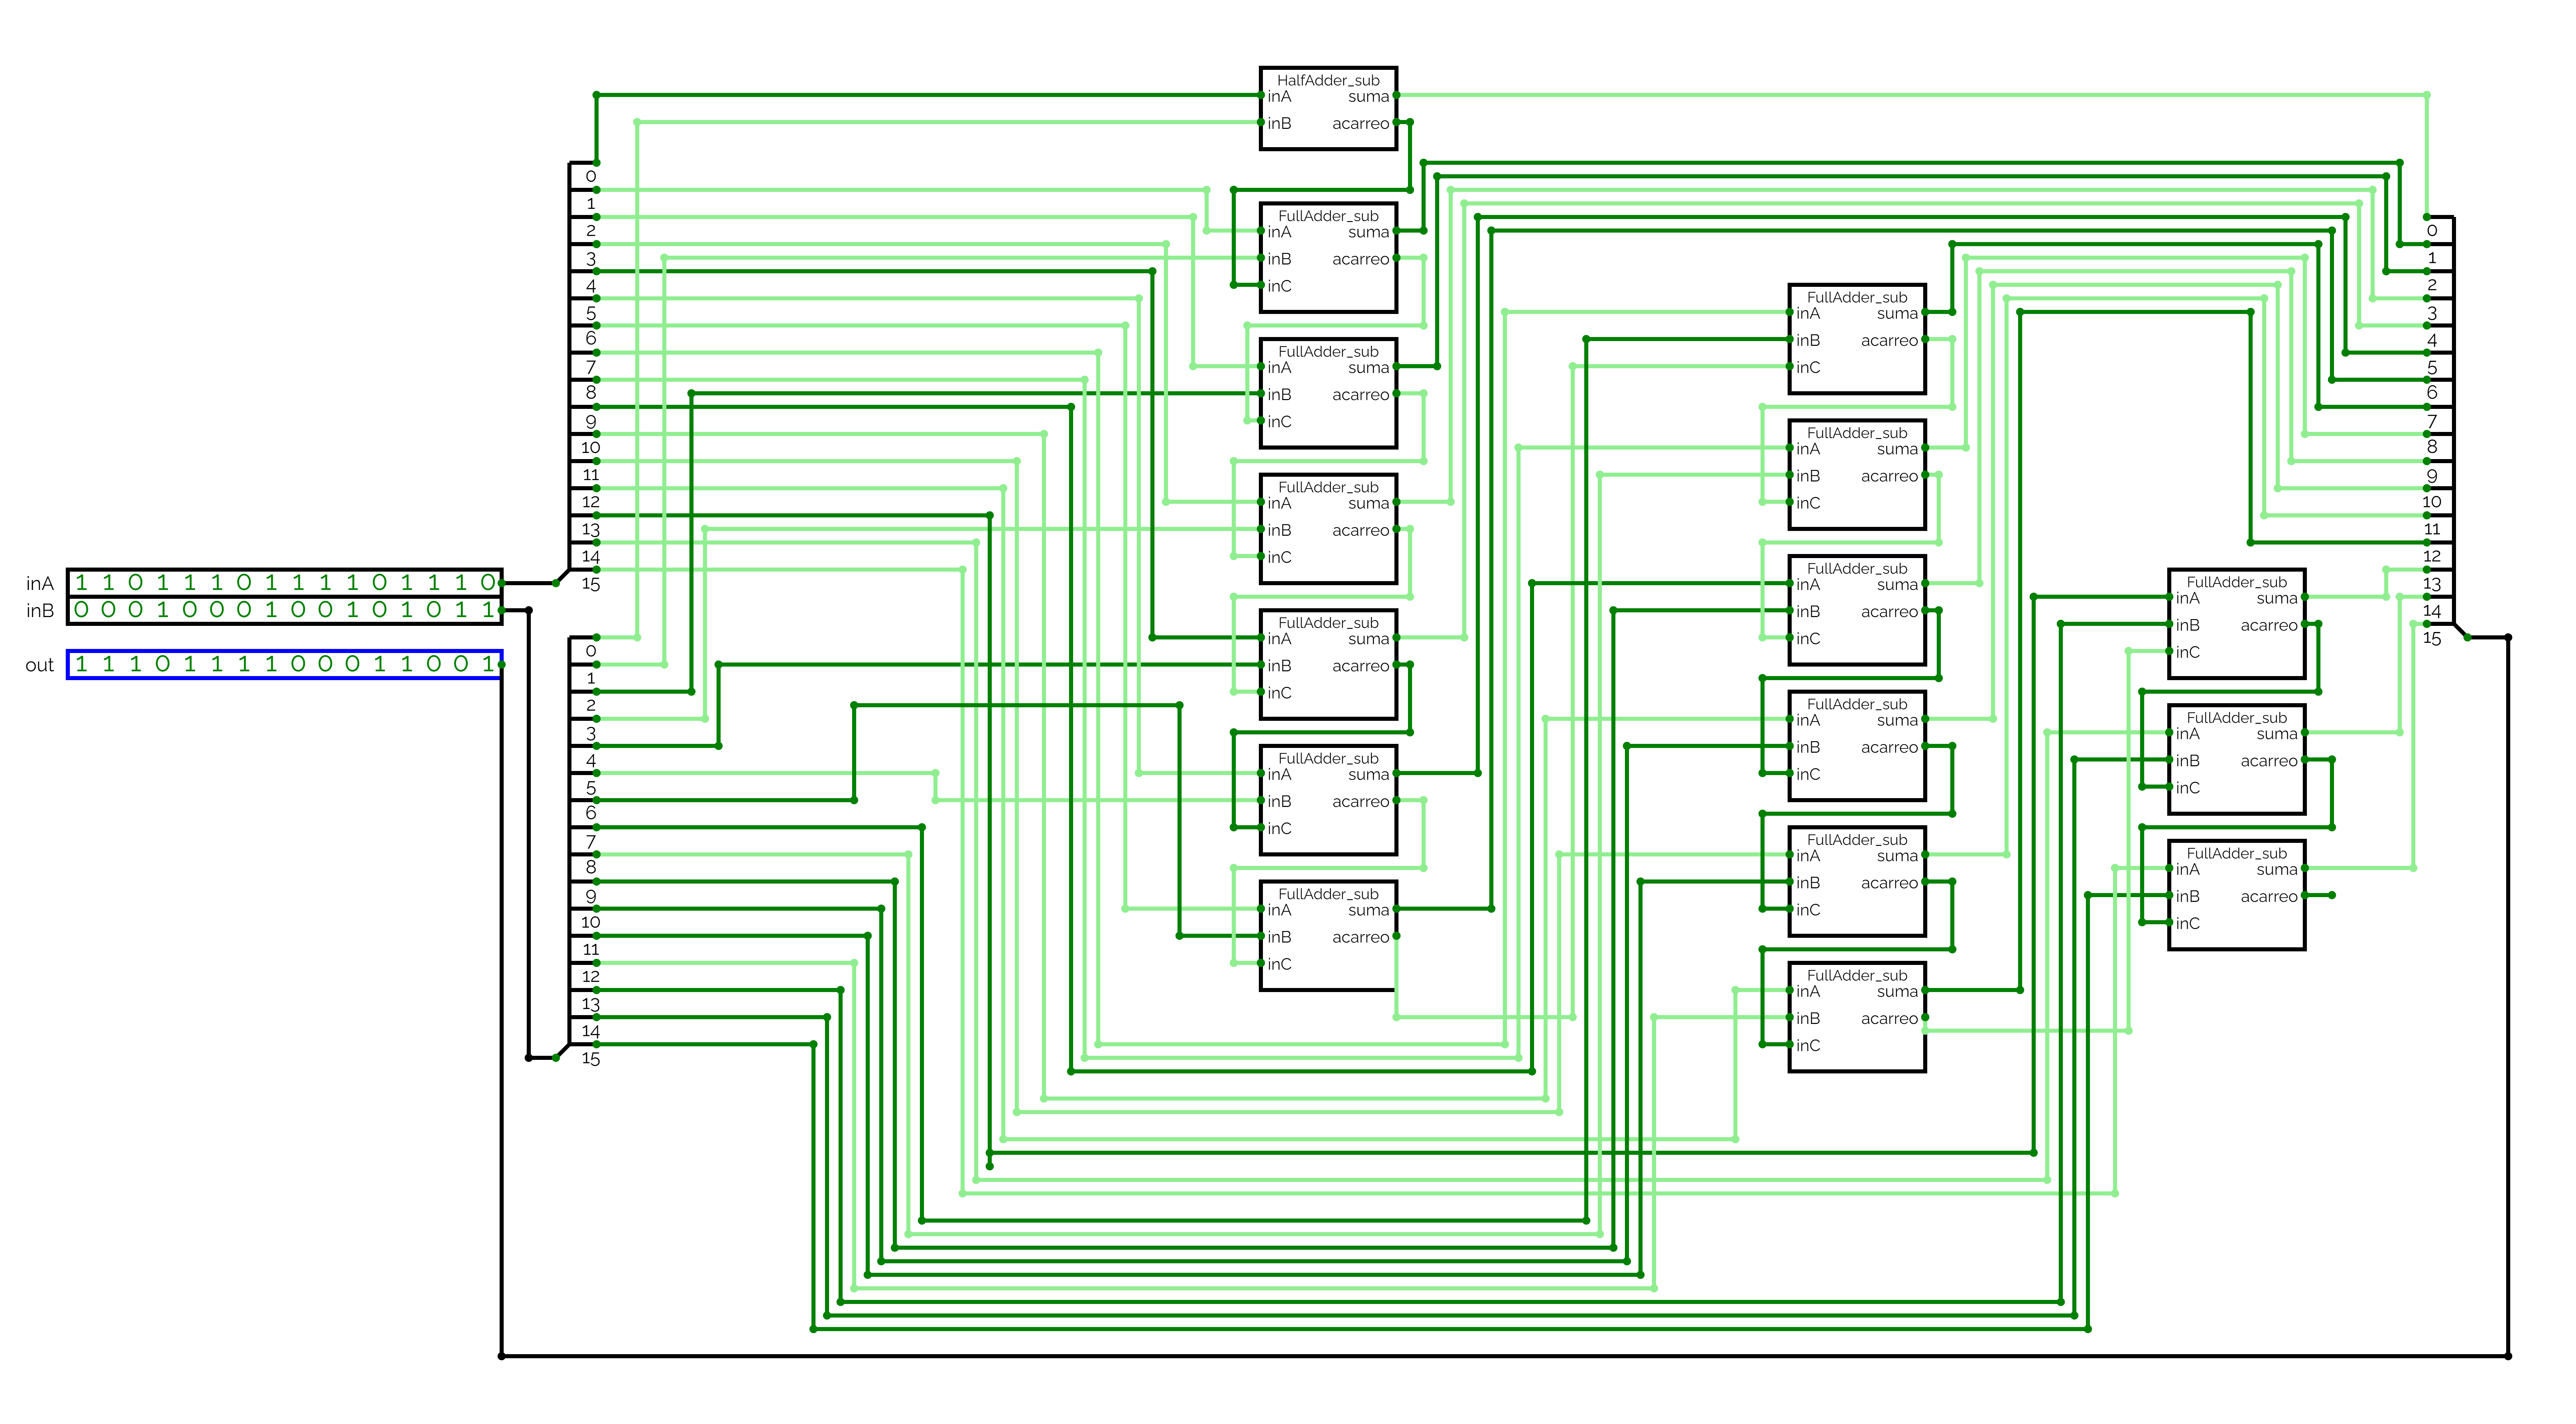
\includegraphics[width=0.75\linewidth]{ALU/16-bitadder_ int.png}
	\caption{Esquema interior del circuito Add16}
	\label{fig:f_add16}
\end{figure}
\subsection{Implementación HDL}
\begin{figure}[H]
	\centering
	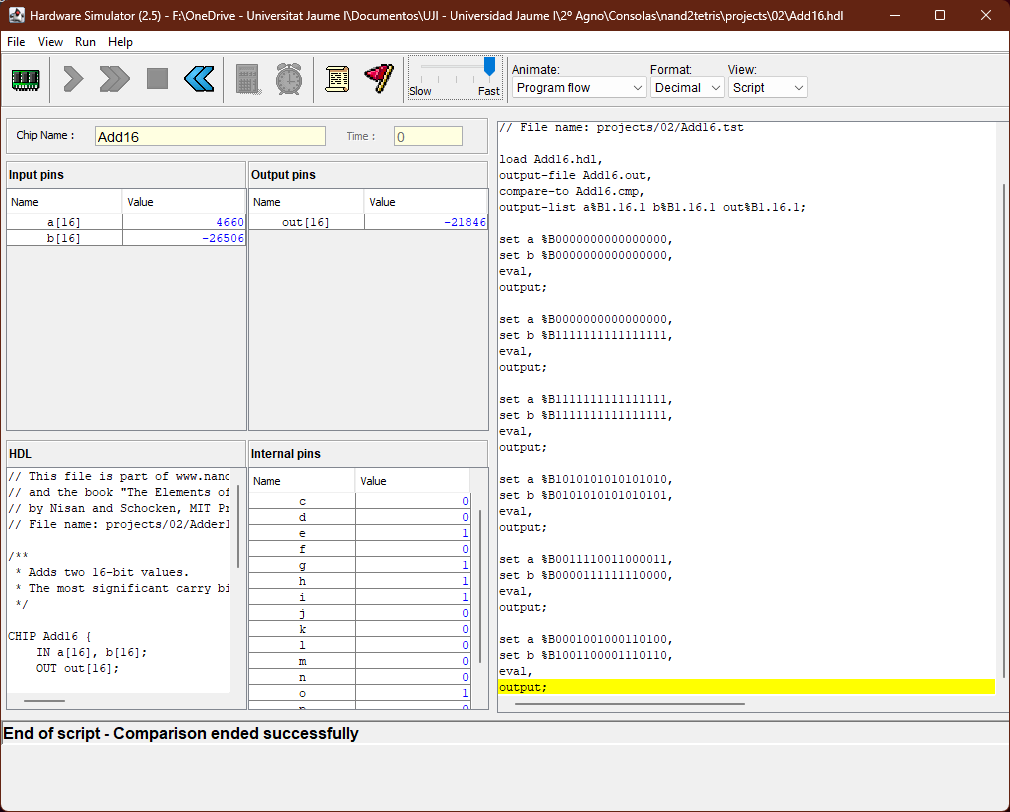
\includegraphics[width=0.75\linewidth]{ALU/add16_hw.png}
	\caption{Test de Add16}
	\label{fig:enter-label}
\end{figure}
\newpage
\subsubsection{Archivo .HDL}
\begin{lstlisting}

	CHIP Add16 {
		IN a[16], b[16];
		OUT out[16];

		PARTS:
		HalfAdder(a=a[0],b=b[0],sum=out[0],carry=c);
		FullAdder(a=a[1],b=b[1],c=c,sum=out[1],carry=d);
		FullAdder(a=a[2],b=b[2],c=d,sum=out[2],carry=e);
		FullAdder(a=a[3],b=b[3],c=e,sum=out[3],carry=f);
		FullAdder(a=a[4],b=b[4],c=f,sum=out[4],carry=g);
		FullAdder(a=a[5],b=b[5],c=g,sum=out[5],carry=h);
		FullAdder(a=a[6],b=b[6],c=h,sum=out[6],carry=i);
		FullAdder(a=a[7],b=b[7],c=i,sum=out[7],carry=j);
		FullAdder(a=a[8],b=b[8],c=j,sum=out[8],carry=k);
		FullAdder(a=a[9],b=b[9],c=k,sum=out[9],carry=l);
		FullAdder(a=a[10],b=b[10],c=l,sum=out[10],carry=m);
		FullAdder(a=a[11],b=b[11],c=m,sum=out[11],carry=n);
		FullAdder(a=a[12],b=b[12],c=n,sum=out[12],carry=o);
		FullAdder(a=a[13],b=b[13],c=o,sum=out[13],carry=p);
		FullAdder(a=a[14],b=b[14],c=p,sum=out[14],carry=q);
		FullAdder(a=a[15],b=b[15],c=q,sum=out[15],carry=drop);
	}
\end{lstlisting}
\subsubsection{Archivo .TST}
\begin{lstlisting}

	set a %B0000000000000000,
	set b %B0000000000000000,
	eval,
	output;

	set a %B0000000000000000,
	set b %B1111111111111111,
	eval,
	output;

	set a %B1111111111111111,
	set b %B1111111111111111,
	eval,
	output;

	set a %B1010101010101010,
	set b %B0101010101010101,
	eval,
	output;

	set a %B0011110011000011,
	set b %B0000111111110000,
	eval,
	output;

	set a %B0001001000110100,
	set b %B1001100001110110,
	eval,
	output;

\end{lstlisting}


\subsubsection{Archivo .CMP}
\begin{lstlisting}

	|        a         |        b         |       out        |
	| 0000000000000000 | 0000000000000000 | 0000000000000000 |
	| 0000000000000000 | 1111111111111111 | 1111111111111111 |
	| 1111111111111111 | 1111111111111111 | 1111111111111110 |
	| 1010101010101010 | 0101010101010101 | 1111111111111111 |
	| 0011110011000011 | 0000111111110000 | 0100110010110011 |
	| 0001001000110100 | 1001100001110110 | 1010101010101010 |
\end{lstlisting}
\newpage
%%%%%%%%%%%%%%%%%%%%%%%%%%%%%%%%%%%%%%%%%%%%%%%%%%%%%%%%%%%%%%%%%%%%%%%%%%
%%%%%%%%%%%%%%%%%%%%%%%%%%%%%%%%%%%%%%%%%%%%%%%%%%%%%%%%%%%%%%%%%%%%%%%%%%
\section{Inc16}
\subsection{Tabla de verdad y explicación del circuito}
El incrementer es, en pocas palabras, un adder con dos inputs; uno con un número binario de 16-bits y otro con el valor constante de 1. Así que, funciona incrementando el valor A por 1.
\begin{table}[H]
	\centering
	\caption{Tabla de verdad de Inc16}
	\label{tab:fulladder}
	\begin{tblr}{
			width = \linewidth,
			colspec = {Q[471]Q[469]},
			cells = {c, font=\ttfamily}, % Set font to monospaced (typewriter)
			hlines,
			vlines,
			hline{1,6} = {-}{0.08em},
		}
		\texttt{Inputs (A15-A0)}                  & \texttt{Outputs (B15-B0)}                 \\
		\texttt{0000 0000 0000 0000 (Decimal: 0)} & \texttt{0000 0000 0000 0001 (Decimal: 1)} \\
		\ldots                                   & \ldots                                    \\
		\texttt{1111 1111 1111 1110 (Decimal: 65534)} & \texttt{1111 1111 1111 1111 (Decimal: 65535)} \\
		\texttt{1111 1111 1111 1111 (Decimal: 65535)} & \texttt{0000 0000 0000 0000 (Decimal: 0)}
	\end{tblr}
\end{table}

\subsection{Esquema del circuito exterior y exterior}

\subsubsection{Interior}
\begin{figure}[H]
	\centering
	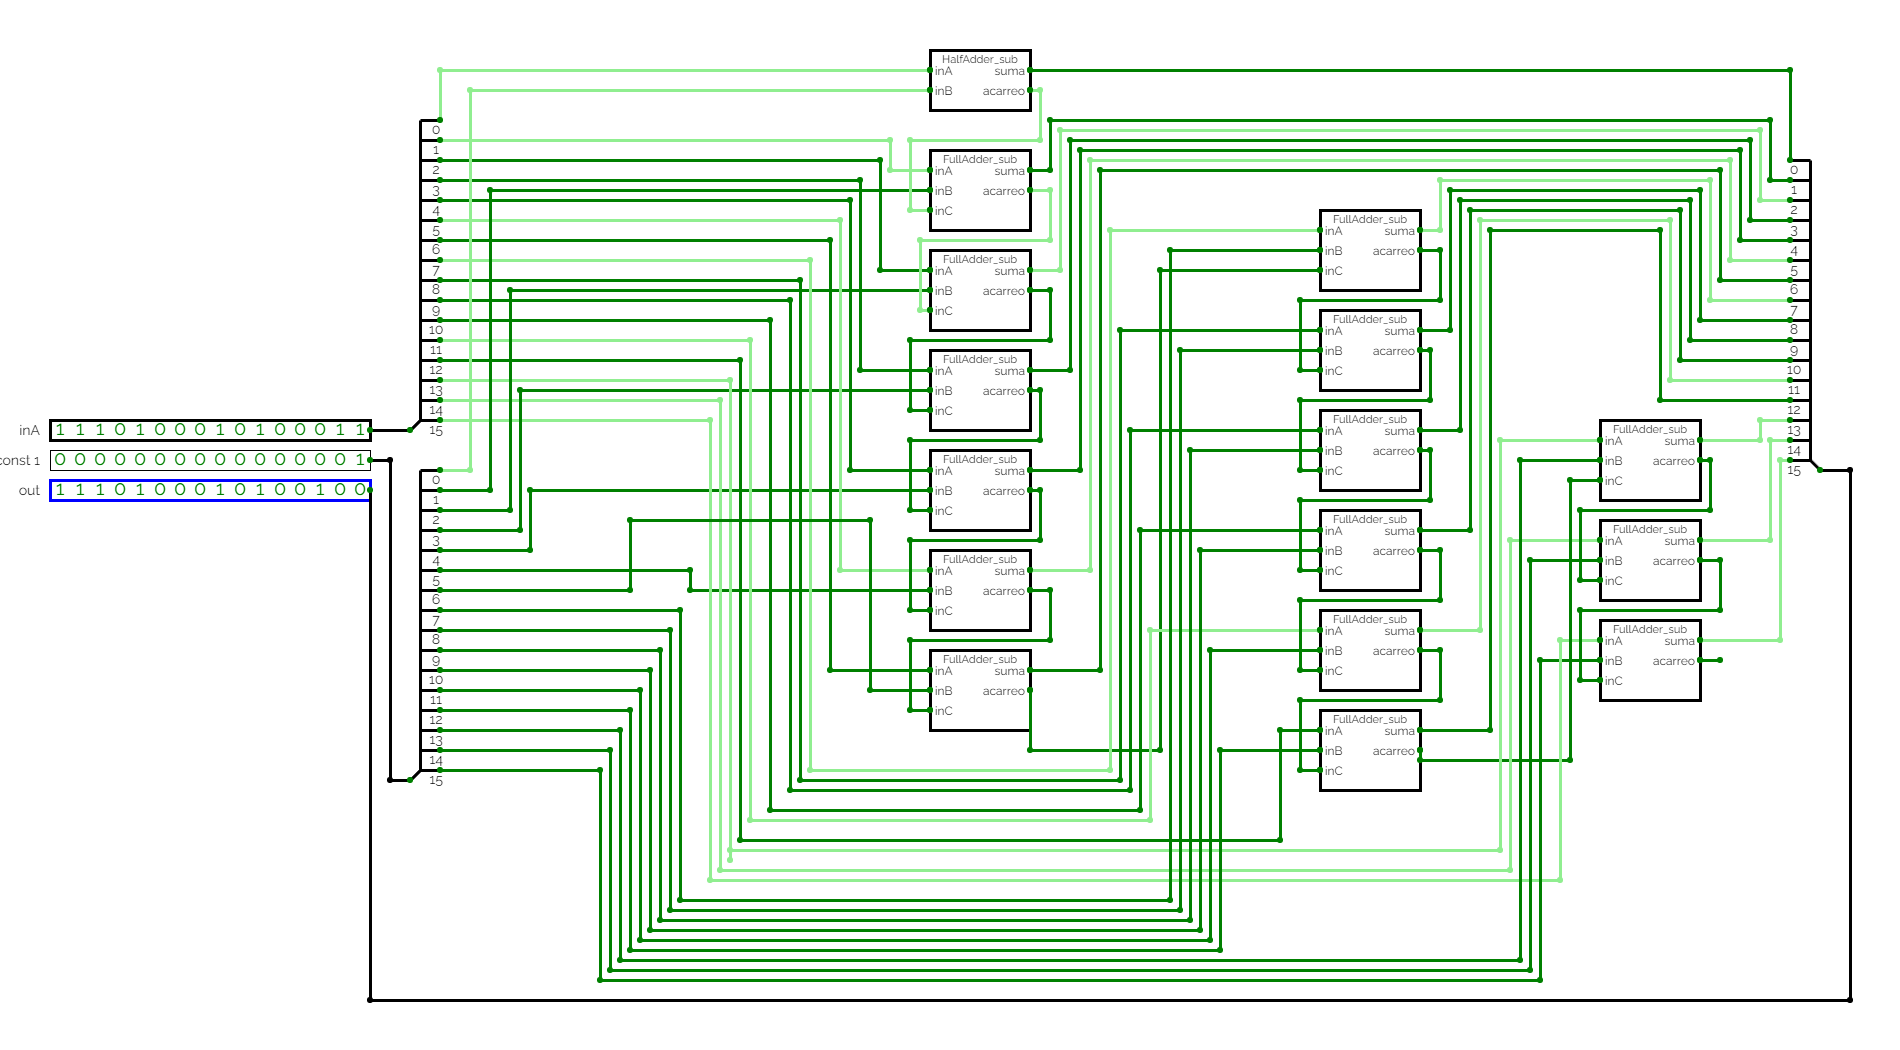
\includegraphics[width=0.75\linewidth]{ALU/Incrementer_int.png}
	\caption{Esquema interior del circuito Inc16}
	\label{fig:f_Inc16}
\end{figure}
\subsection{Implementación HDL}
\begin{figure}[H]
	\centering
	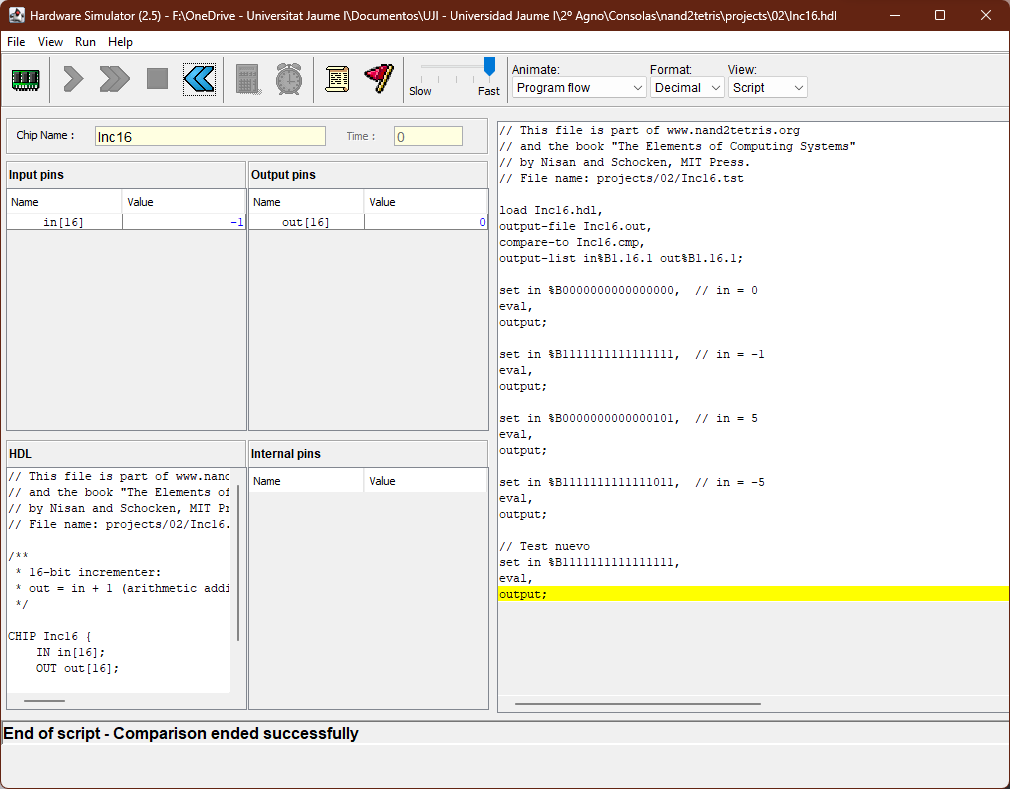
\includegraphics[width=0.75\linewidth]{ALU/inc16_hw.png}
	\caption{Test de Inc16}
	\label{fig:enter-label}
\end{figure}
\subsubsection{Archivo .HDL}
\begin{lstlisting}

	CHIP Inc16 {
		IN in[16];
		OUT out[16];

		PARTS:
		Add16(a=in,b[0]=true,out=out);
	}
\end{lstlisting}
\subsubsection{Archivo .TST}
\begin{lstlisting}

	load Inc16.hdl,
	output-file Inc16.out,
	compare-to Inc16.cmp,
	output-list in%B1.16.1 out%B1.16.1;

	set in %B0000000000000000,  // in = 0
	eval,
	output;

	set in %B1111111111111111,  // in = -1
	eval,
	output;

	set in %B0000000000000101,  // in = 5
	eval,
	output;

	set in %B1111111111111011,  // in = -5
	eval,
	output;

	// Test nuevo
	set in %B1111111111111111,
	eval,
	output;


\end{lstlisting}

\subsubsection{Archivo .CMP}
\begin{lstlisting}
	|        in        |       out        |
	| 0000000000000000 | 0000000000000001 |
	| 1111111111111111 | 0000000000000000 |
	| 0000000000000101 | 0000000000000110 |
	| 1111111111111011 | 1111111111111100 |
	| 1111111111111111 | 0000000000000000 |
\end{lstlisting}
\newpage
%%%%%%%%%%%%%%%%%%%%%%%%%%%%%%%%%%%%%%%%%%%%%%%%%%%%%%%%%%%%%%%%%%%%%%%%%%
%%%%%%%%%%%%%%%%%%%%%%%%%%%%%%%%%%%%%%%%%%%%%%%%%%%%%%%%%%%%%%%%%%%%%%%%%%
\section{ALU}
\subsection{Tabla de verdad y explicación del circuito}
La ALU lleva a cabo diferentes operaciones dependiendo del bit que lleven sus multiples inputs.
% \usepackage{color}
% \usepackage{tabularray}
\begin{table}[H]
	\centering
	\caption{Tabla de verdad de Add16}
	\label{tab:fulladder}
	\begin{tblr}{
			width = \linewidth,
			colspec = {Q[123]Q[67]Q[94]Q[96]Q[185]Q[285]Q[83]},
			cells = {c, font=\ttfamily}, % Set font to monospaced (typewriter)
			cell{1}{1} = {c=2}{0.19\linewidth},
			cell{1}{3} = {c=2}{0.19\linewidth},
			hline{1,13} = {-}{0.08em},
			hline{2,4} = {-}{},
		}
		{Estos bits dicen \\como preajustar \\el input x} &  & {Estos bits dicen\\como preajustar\\el input x } &  & {El bit seleciona~\\entre + / And} & {Este bit selecciona como\\producir el output} & \\
		zx & nx & zy & ny & f & no & out\\
		{if zx then\\x = 0} & {if nx\\then\\x=!x} & {if zy\\then\\y=0} & {if ny\\then\\y=!y} & {if f then\\out=x+y\\else\\out=xy} & {if no\\then\\out=!out} & f(x,y)=\\
		0 & 1 & 1 & 1 & 1 & 1 & x+1\\
		1 & 1 & 0 & 1 & 1 & 1 & y+1\\
		0 & 0 & 1 & 1 & 1 & 0 & x-1\\
		1 & 1 & 0 & 0 & 1 & 0 & y-1\\
		0 & 0 & 0 & 0 & 1 & 0 & x+y\\
		0 & 1 & 0 & 0 & 1 & 1 & x-y\\
		0 & 0 & 0 & 1 & 1 & 1 & y-x\\
		0 & 0 & 0 & 0 & 0 & 0 & xy\\
		0 & 1 & 0 & 1 & 0 & 1 & x\textbar{}y
	\end{tblr}
\end{table}
\subsection{Esquema del circuito exterior y exterior}
\subsubsection{Exterior}
\begin{figure}[H]
	\centering
	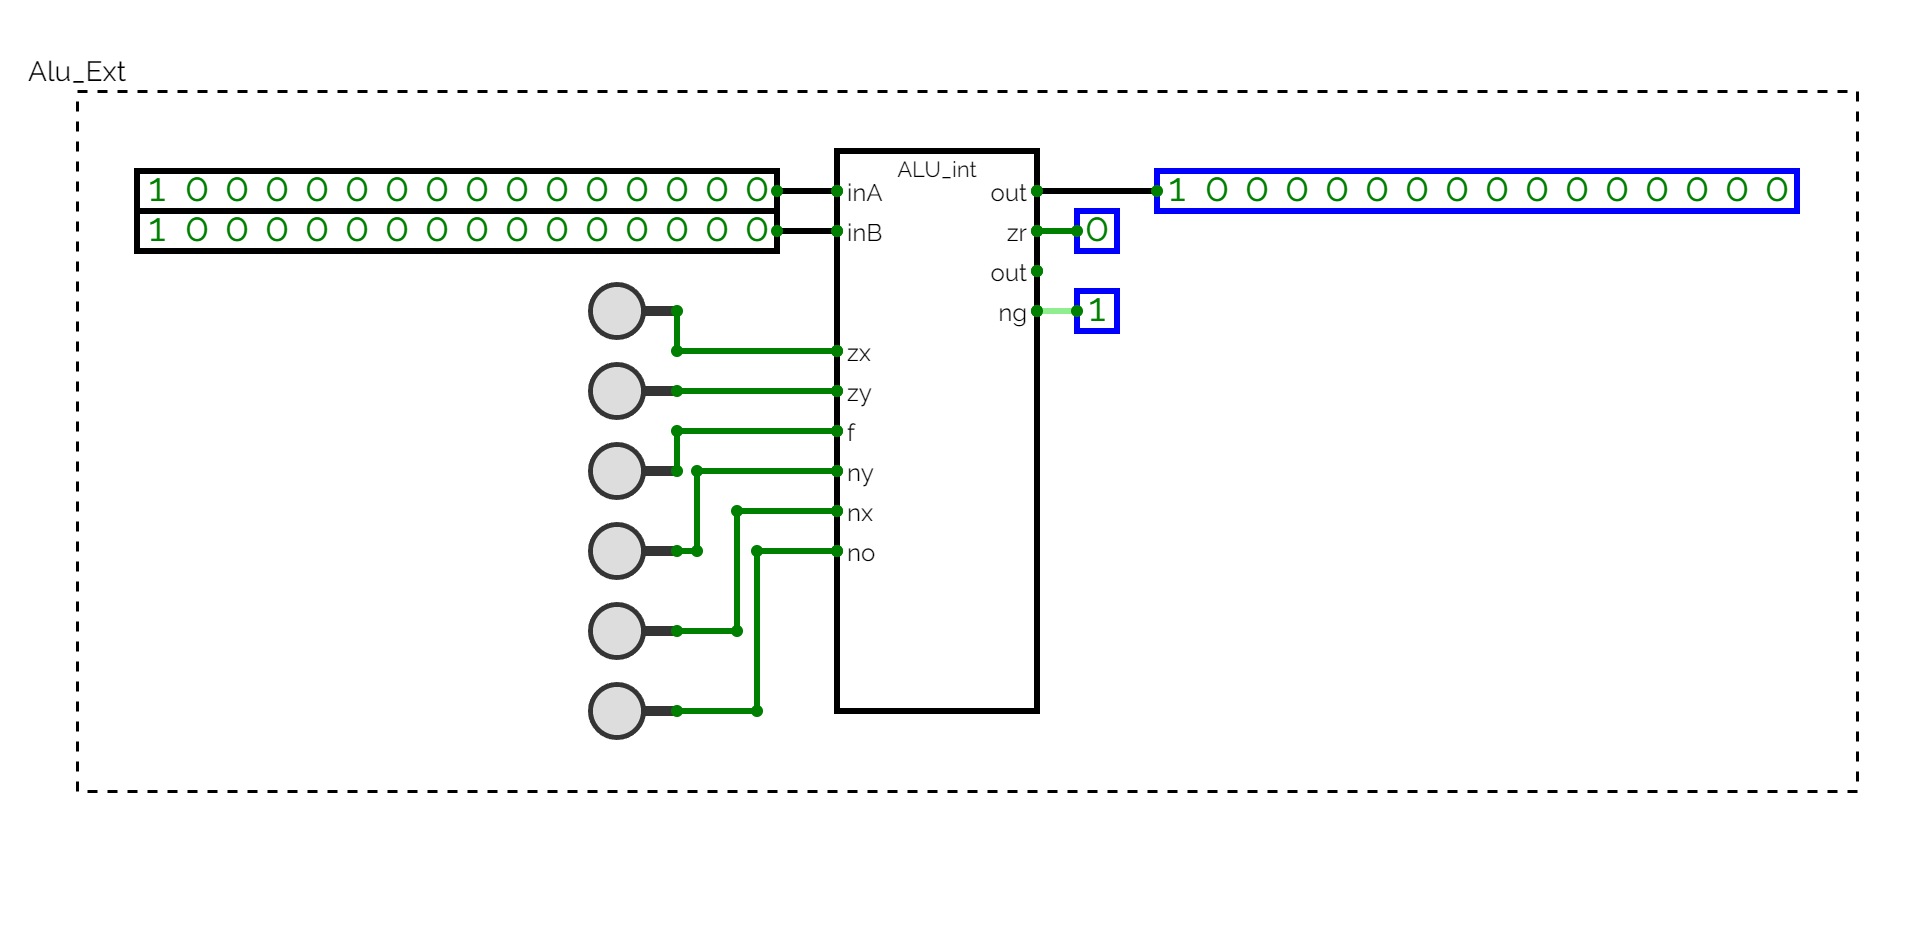
\includegraphics[width=0.75\linewidth]{ALU/ALU_ext.png}
	\caption{Esquema exterior de una ALU}
	\label{fig:Inc16}
\end{figure}
\subsubsection{Interior}
\begin{figure}[H]
	\centering
	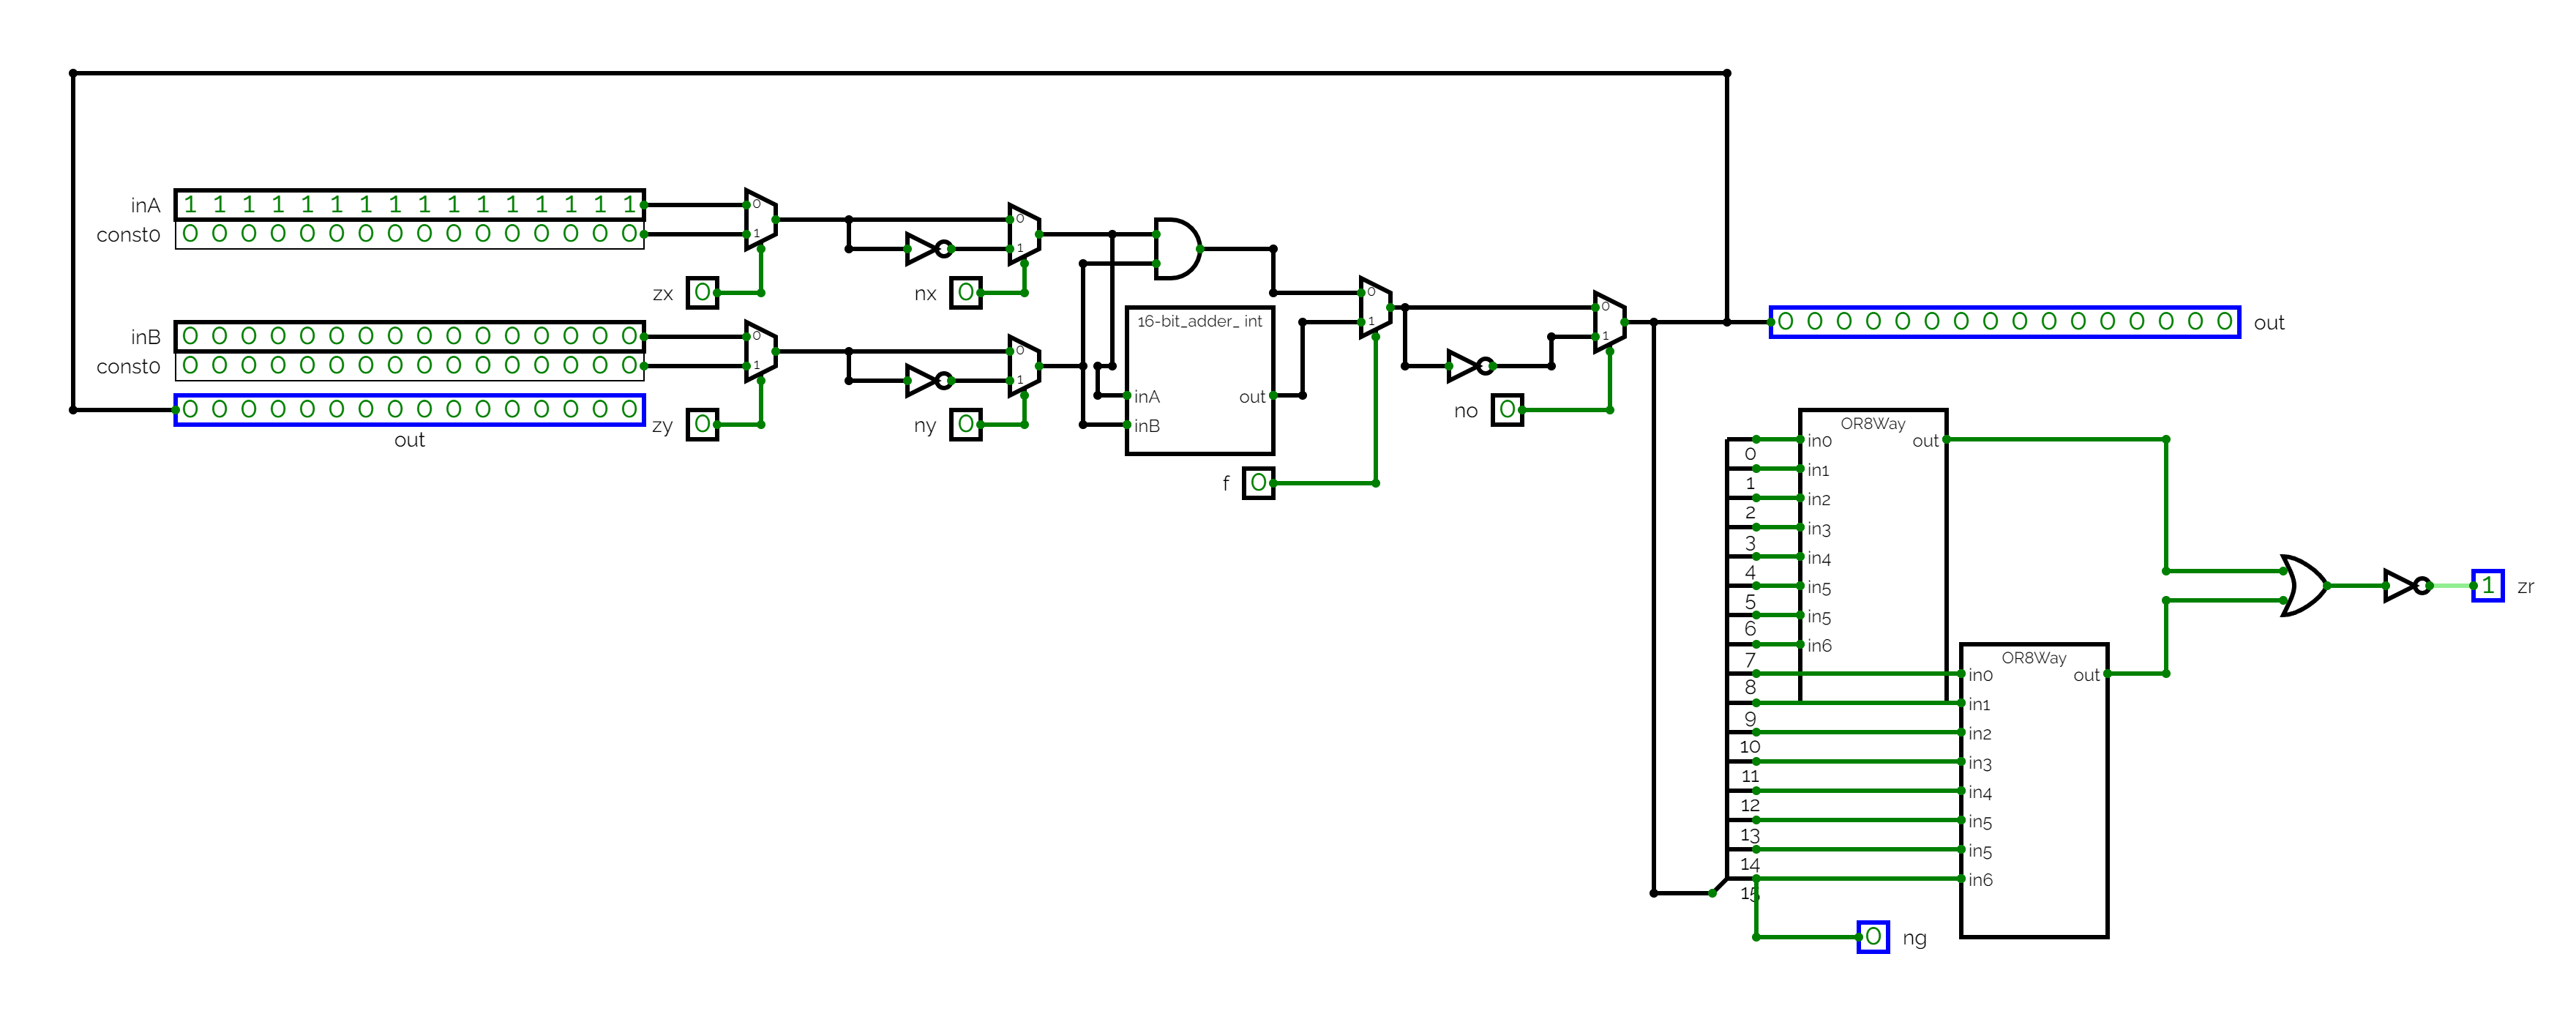
\includegraphics[width=0.75\linewidth]{ALU/ALU_int.png}
	\caption{Esquema interior de una ALU}
	\label{fig:f_Inc16}
\end{figure}
\subsection{Implementación HDL}
\begin{figure}[H]
	\centering
	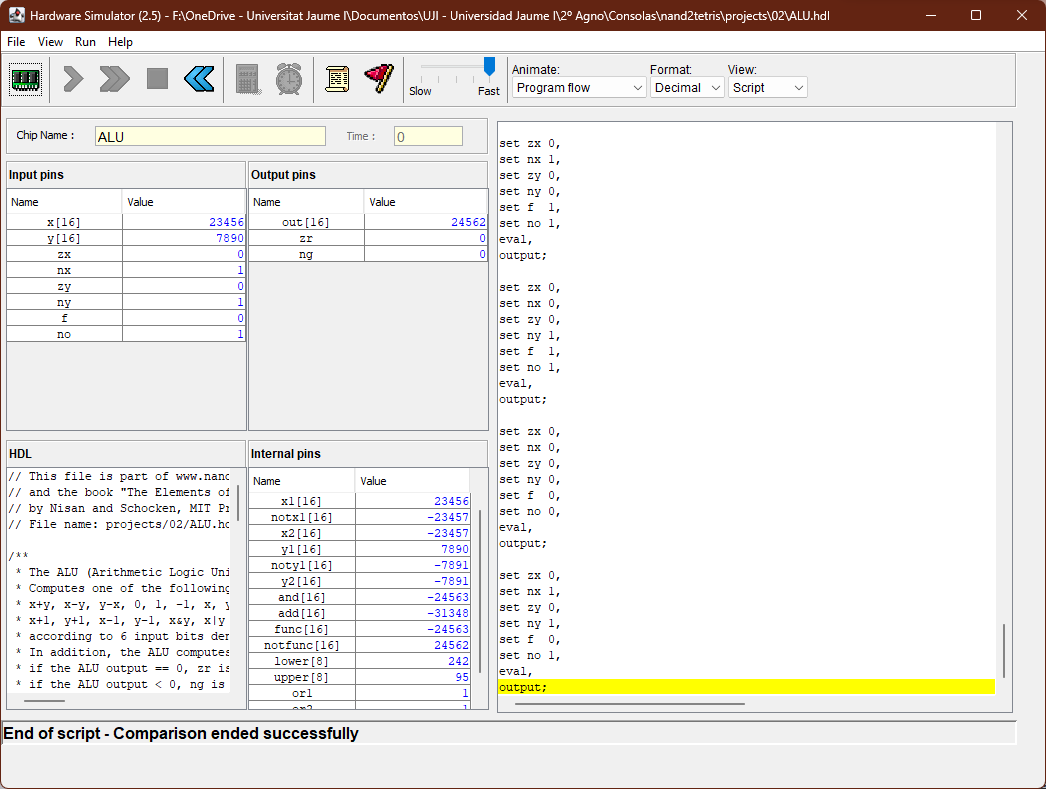
\includegraphics[width=0.75\linewidth]{ALU/alu_hw.png}
	\caption{Test de ALU}
	\label{fig:enter-label}
\end{figure}
\subsubsection{Archivo .HDL}
\begin{lstlisting}
	CHIP ALU {
		IN
		x[16], y[16],  // 16-bit inputs
		zx, // zero the x input?
		nx, // negate the x input?
		zy, // zero the y input?
		ny, // negate the y input?
		f,  // compute  out = x + y (if f == 1) or out = x & y (if == 0)
		no; // negate the out output?

		OUT
		out[16], // 16-bit output
		zr, // 1 if (out == 0), 0 otherwise
		ng; // 1 if (out < 0),  0 otherwise

		PARTS:
		// zx
		Mux16(a=x, b=false, sel=zx, out=x1);

		// nx
		Not16(in=x1, out=notx1);
		Mux16(a=x1, b=notx1, sel=nx, out=x2);

		// zy
		Mux16(a=y, b=false, sel=zy, out=y1);

		// ny
		Not16(in=y1, out=noty1);
		Mux16(a=y1, b=noty1, sel=ny, out=y2);

		// f
		And16(a=x2, b=y2, out=and);
		Add16(a=x2, b=y2, out=add);
		Mux16(a=and, b=add, sel=f, out=func);

		// no, ng
		Not16(in=func, out=notfunc);
		Mux16(a=func, b=notfunc, sel=no, out=out, out[0..7]=lower, out[8..15]=upper, out[15]=ng);

		// zr
		Or8Way(in=lower, out=or1);
		Or8Way(in=upper, out=or2);
		Or(a=or1, b=or2, out=or);
		Not(in=or, out=zr);
	}
\end{lstlisting}
\subsubsection{Archivo .TST}
\begin{lstlisting}
	// Tests viejos
	. . .
	// Test nuevo
	set x %B0000000000000000,  // x = 0
	set y %B1111111111111111,  // y = -1

	// Operacion AND
	set zx 1,
	set nx 0,
	set zy 1,
	set ny 0,
	set f  0,
	set no 0,
	eval,
	output;}
	\end{lstlisting}
	\subsubsection{Archivo .CMP}
	\begin{lstlisting}
// Comparers viejos
...
// Comprarer nuevo
|        x         |        y         |zx |nx |zy |ny | f |no |       out        |zr |ng |
| 0000000000000000 | 1111111111111111 | 1 | 0 | 1 | 0 | 0 | 0 | 0000000000000000 | 1 | 0 |
\end{lstlisting}
\newpage

%%%%%%%%%%%%%%%%%%%%%%%%%%%%%%%%%%%%%%%%%%%%%%%%%%%%%%%%%%%%%%%%%%%%%%%%%%
%%%%%%%%%%%%%%%%%%%%%%%%%%%%%%%%%%%%%%%%%%%%%%%%%%%%%%%%%%%%%%%%%%%%%%%%%%
\section{Registro de 1bit}
\subsection{Tabla de verdad y explicación del circuito}

El registro de 1bit se compone de dos piezas fundamentales, el \textit{data flip flop} (DFF) y un MUX que sirve como el selector de escritura o lectura.
Esta pieza sirve para almacenar (o recordar \cite{nisan_nand2tetris_2005}) un valor durante un tiempo.
% \usepackage{tabularray}
\begin{table}[H]
	\centering
	\caption{Tabla de verdad de registro de 1bit \cite{chatgpt}}
	\label{tab:1bit}
	\begin{tblr}{
			width = \linewidth,
			colspec = {Q[198]Q[183]Q[475]},
			cells = {c, font=\ttfamily},
			hline{1,5} = {-}{0.08em},
		}
		\textbf{Load} & \textbf{Data} & \textbf{Q (next state)}\\
		0 & X & Q (no change)\\
		1 & 0 & 0\\
		1 & 1 & 1
	\end{tblr}
\end{table}
\subsection{Esquema del circuito exterior y exterior}
\begin{figure}[H]
	\centering
	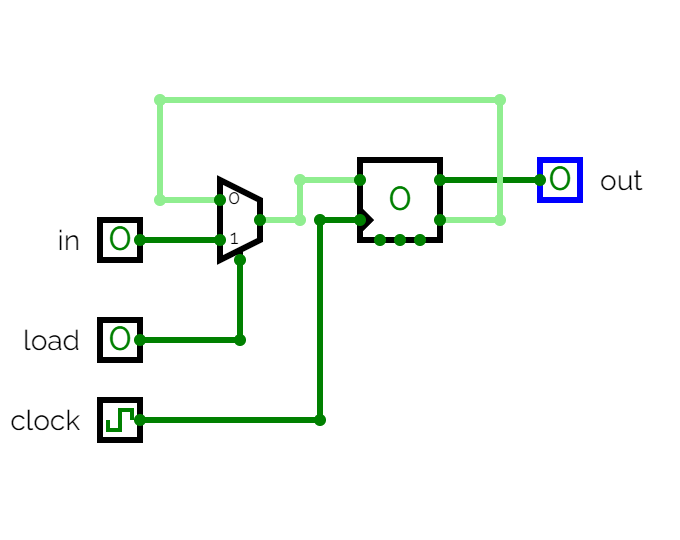
\includegraphics[width=0.75\linewidth]{RAM/REG1Bit.png}
	\caption{Esquema interior de un registro de 1 bit.}
	\label{fig:reg1bit}
\end{figure}
\subsection{Implementación HDL}
\begin{figure}[H]
	\centering
	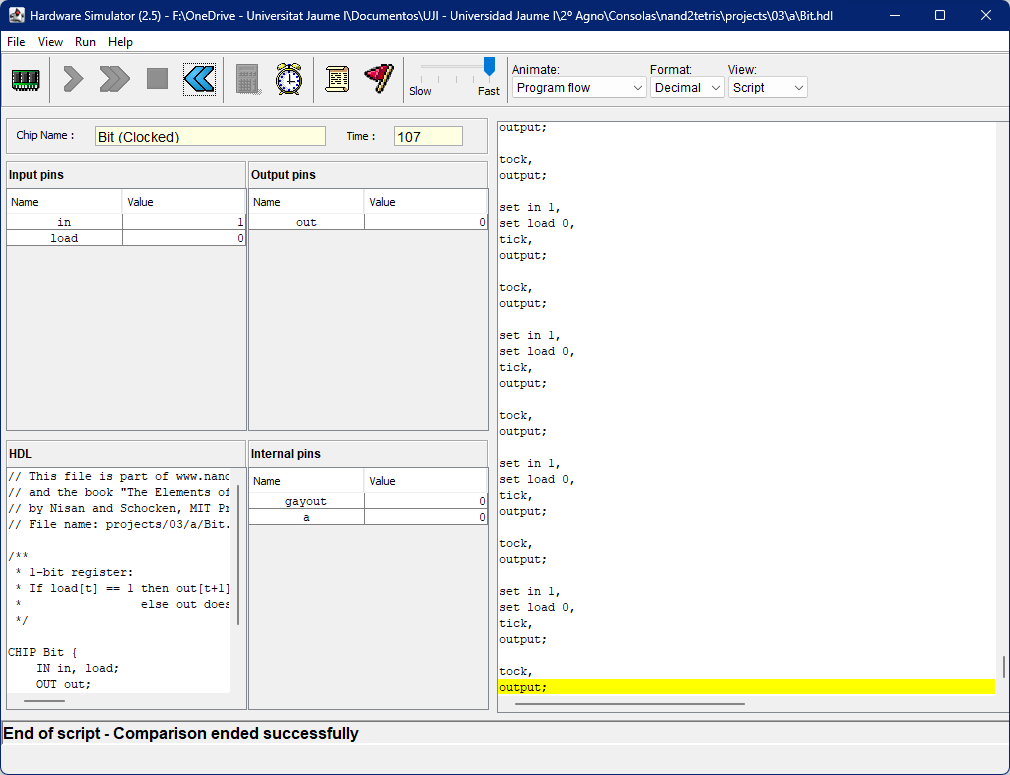
\includegraphics[width=0.75\linewidth]{RAM/bit_hdl}
	\caption{Implementación en Hardware Simulator de Registro de 1bit}
	\label{fig:bithdl}
\end{figure}
\subsubsection{Archivo .HDL}
\begin{lstlisting}
	CHIP Bit {
		IN in, load;
		OUT out;

		PARTS:
		Mux(a=gayout,b=in,sel=load,out=a);
		DFF(in=a,out=out,out=gayout);
	}
\end{lstlisting}

\newpage
%%%%%%%%%%%%%%%%%%%%%%%%%%%%%%%%%%%%%%%%%%%%%%%%%%%%%%%%%%%%%%%%%%%%%%%%%%
%%%%%%%%%%%%%%%%%%%%%%%%%%%%%%%%%%%%%%%%%%%%%%%%%%%%%%%%%%%%%%%%%%%%%%%%%%
\section{REG16}
\subsection{Tabla de verdad y explicación del circuito}
Un registro de 16bit se crea mediante la conjunción de varios (16 en concreto) registros de 1bit.

\begin{table}[H]
	\centering
	\caption{Tabla de verdad registro de 16Bit  \cite{chatgpt}}
	\label{tab:fulladder}
	\begin{tblr}{
			width = \linewidth,
			colspec = {Q[112]Q[402]Q[402]},
			row{even} = {c},
			row{1} = {c},
			row{3} = {c},
			row{5} = {c},
			row{7} = {c},
			row{9} = {c},
			cell{11}{1} = {c},
			cell{11}{2} = {c},
			cell{11}{3} = {c},
			hline{1,13} = {-}{0.08em},
			cells = {font=\ttfamily},
		}
		\textbf{Load} & \textbf{Data[15:0]} & \textbf{Q[15:0] (next state)}\\
		0 & X & Q[15:0] (no change)\\
		1 & 0000 0000 0000 0000 & 0000 0000 0000 0000\\
		1 & 0000 0000 0000 0001 & 0000 0000 0000 0001\\
		1 & 0000 0000 0000 0010 & 0000 0000 0000 0010\\
		1 & 0000 0000 0000 0011 & 0000 0000 0000 0011\\
		1 & 0000 0000 0000 0100 & 0000 0000 0000 0100\\
		1 & 0000 0000 0000 0101 & 0000 0000 0000 0101\\
		1 & 0000 0000 0000 0110 & 0000 0000 0000 0110\\
		1 & 0000 0000 0000 0111 & 0000 0000 0000 0111\\
		... & ...               &       ...          \\
		1 & 1111 1111 1111 1111 & 1111 1111 1111 1111
	\end{tblr}
\end{table}
\subsection{Esquema del circuito exterior y exterior}
\begin{figure}[H]
	\centering
	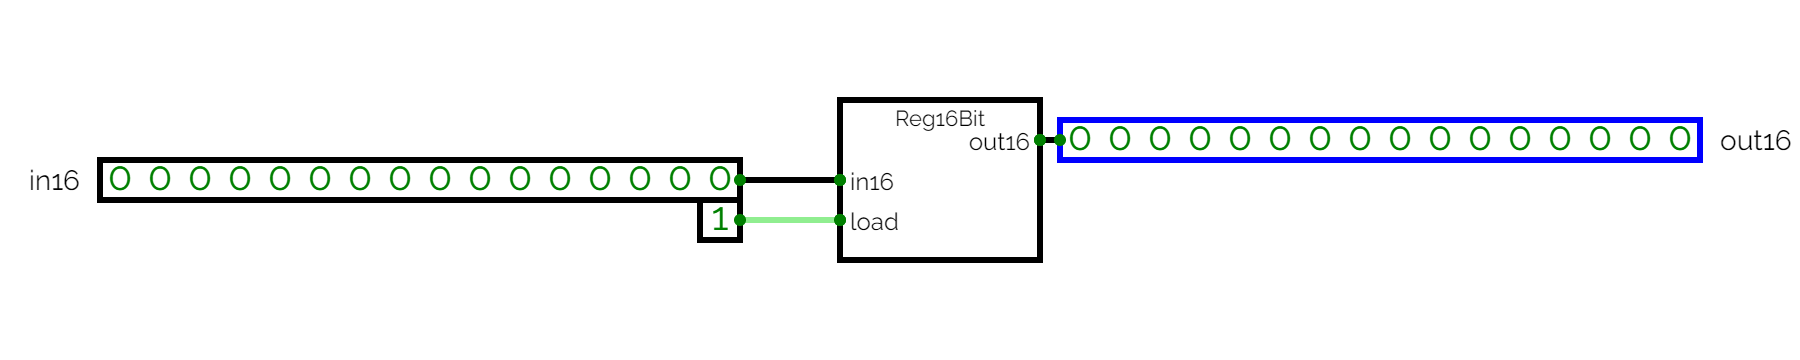
\includegraphics[width=0.75\linewidth]{RAM/REG16bit_ext}
	\caption{Circuito externo de REG16}
	\label{fig:reg16bitext}
\end{figure}

\begin{figure}[H]
	\centering
	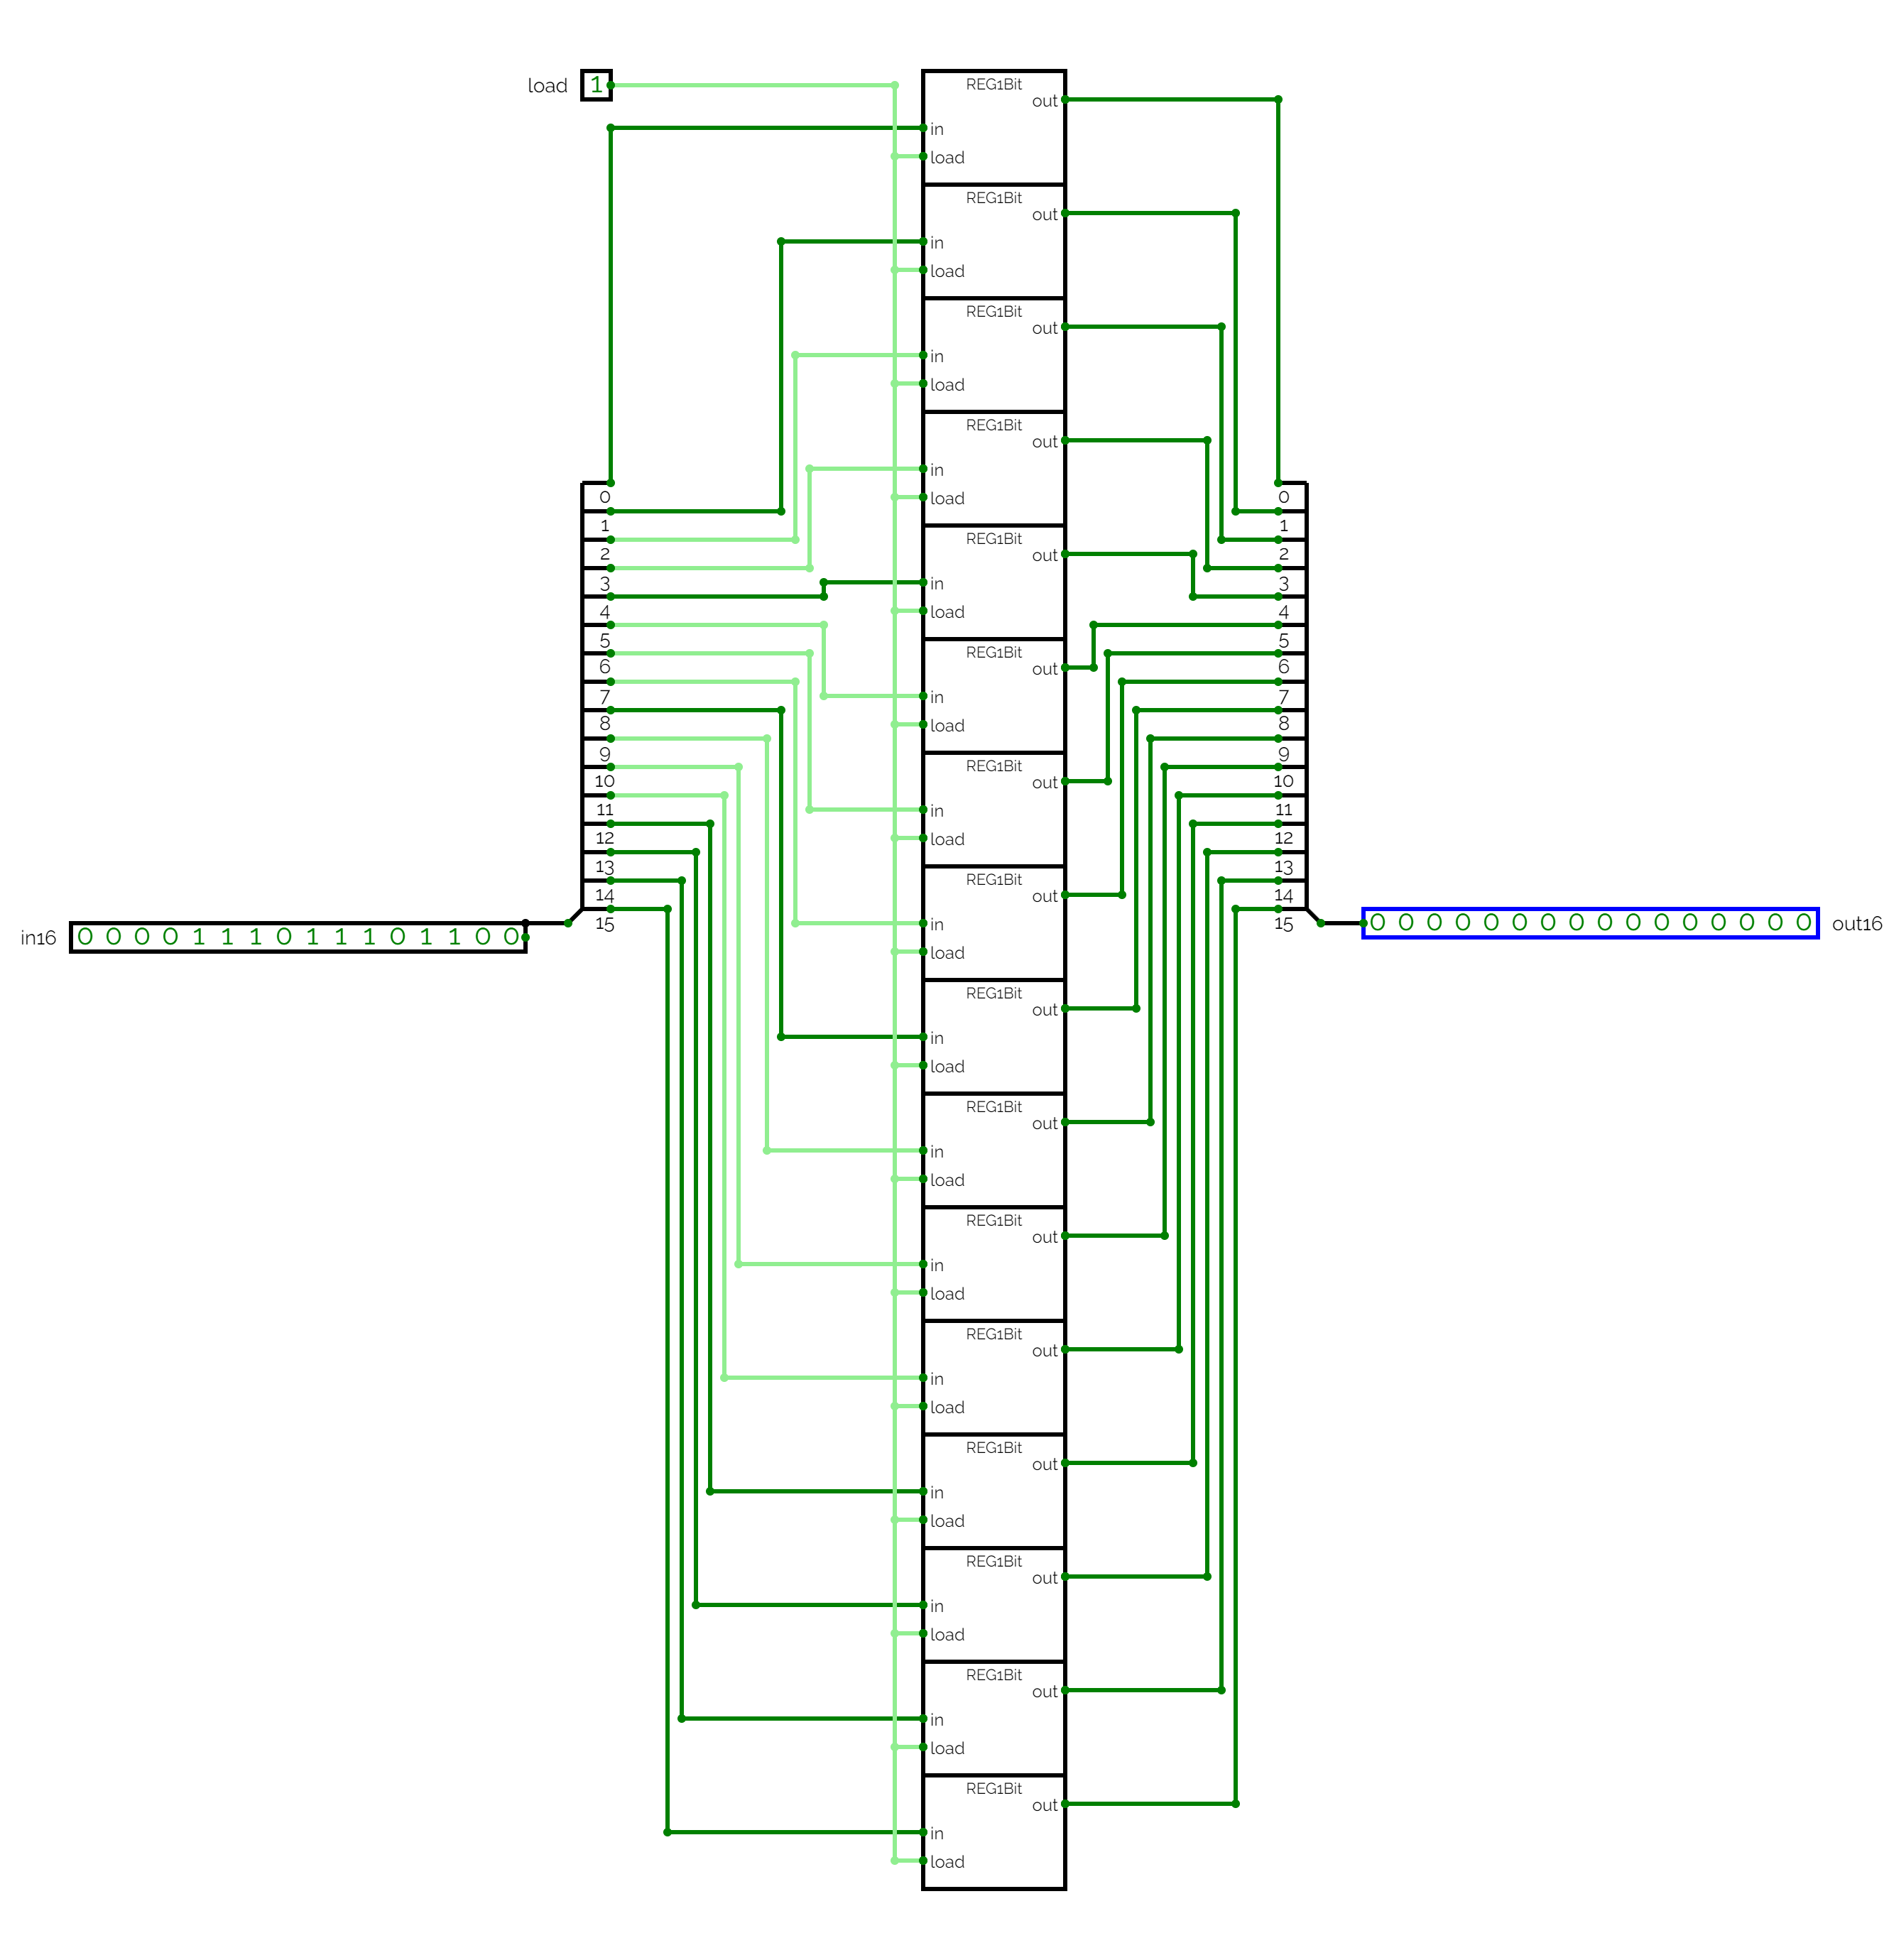
\includegraphics[width=0.75\linewidth]{RAM/Reg16Bit}
	\caption{Circuito interno de REG16}
	\label{fig:reg16bit}
\end{figure}

\subsection{Implementación HDL}
\begin{figure}[H]
	\centering
	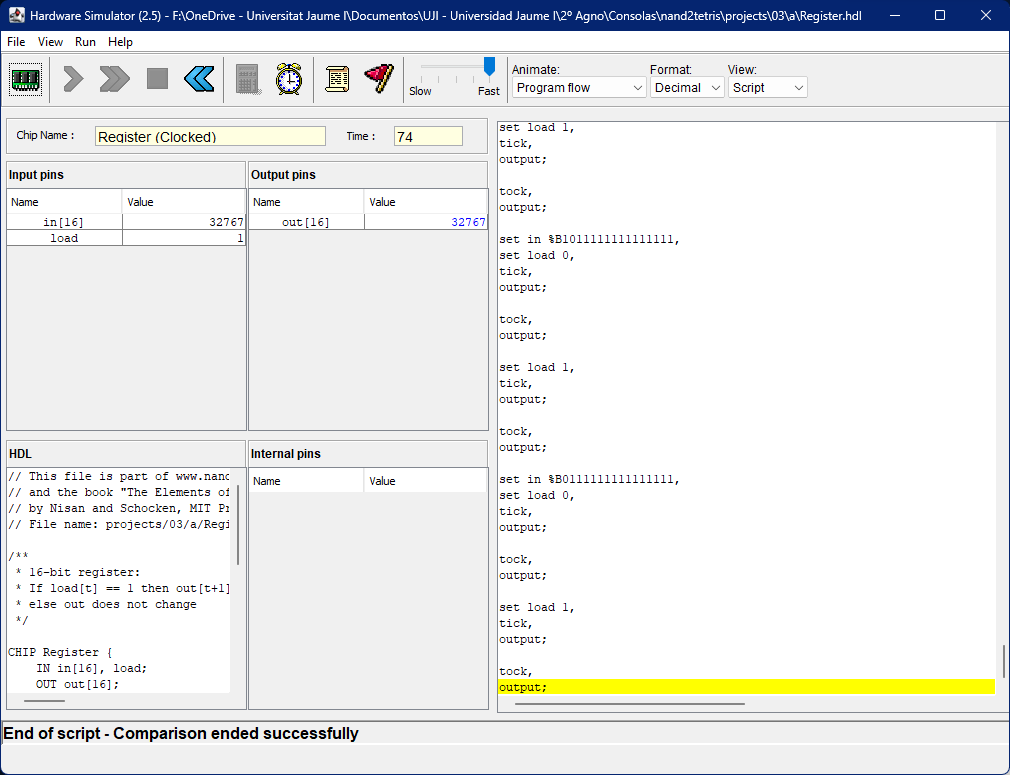
\includegraphics[width=0.75\linewidth]{RAM/reg_hdl}
	\caption{Implementación en Hardware Simulator de REG16}
	\label{fig:reghdl}
\end{figure}

\subsubsection{Archivo .HDL}
\begin{lstlisting}
	CHIP Bit {
		IN in, load;
		OUT out;

		PARTS:
		Mux(a=gayout,b=in,sel=load,out=a);
		DFF(in=a,out=out,out=gayout);
	}
\end{lstlisting}

\newpage
%%%%%%%%%%%%%%%%%%%%%%%%%%%%%%%%%%%%%%%%%%%%%%%%%%%%%%%%%%%%%%%%%%%%%%%%%%
%%%%%%%%%%%%%%%%%%%%%%%%%%%%%%%%%%%%%%%%%%%%%%%%%%%%%%%%%%%%%%%%%%%%%%%%%%
\section{RAM8} \label{ram8}
\subsection{Tabla de verdad y explicación del circuito}
Una RAM es un conjunto de registros n y w-bit, siendo n la cantidad de registros y w la cantidad de bits por registro.
La RAM8 se compone de 8 registros, o de 2 RAM4.
\begin{table}[H]
	\centering
	\caption{Tabla de verdad registro de 16Bit \cite{chatgpt}}
	\label{tab:ram8}
	\begin{tblr}{
			width = \linewidth,
			colspec = {Q[88]Q[204]Q[315]Q[323]},
			cells = {c, font=\ttfamily},
			hline{1,11} = {-}{0.08em},
		}
		\textbf{Load} & \textbf{Address[2:0]} & \textbf{In[15:0]} & \textbf{Out[15:0] (next state)}\\
		0 & 000 & X & Out[15:0] (no change)\\
		1 & 000 & 0000 0000 0000 0000 & Data at Address 0\\
		1 & 001 & 0000 0000 0000 0001 & Data at Address 1\\
		1 & 010 & 0000 0000 0000 0010 & Data at Address 2\\
		1 & 011 & 0000 0000 0000 0011 & Data at Address 3\\
		1 & 100 & 0000 0000 0000 0100 & Data at Address 4\\
		1 & 101 & 0000 0000 0000 0101 & Data at Address 5\\
		1 & 110 & 0000 0000 0000 0110 & Data at Address 6\\
		1 & 111 & 0000 0000 0000 0111 & Data at Address 7
	\end{tblr}
\end{table}
\subsection{Esquema del circuito exterior y exterior}
Composición de una RAM4 con 4 registros de 16bit.
\begin{figure}[H]
	\centering
	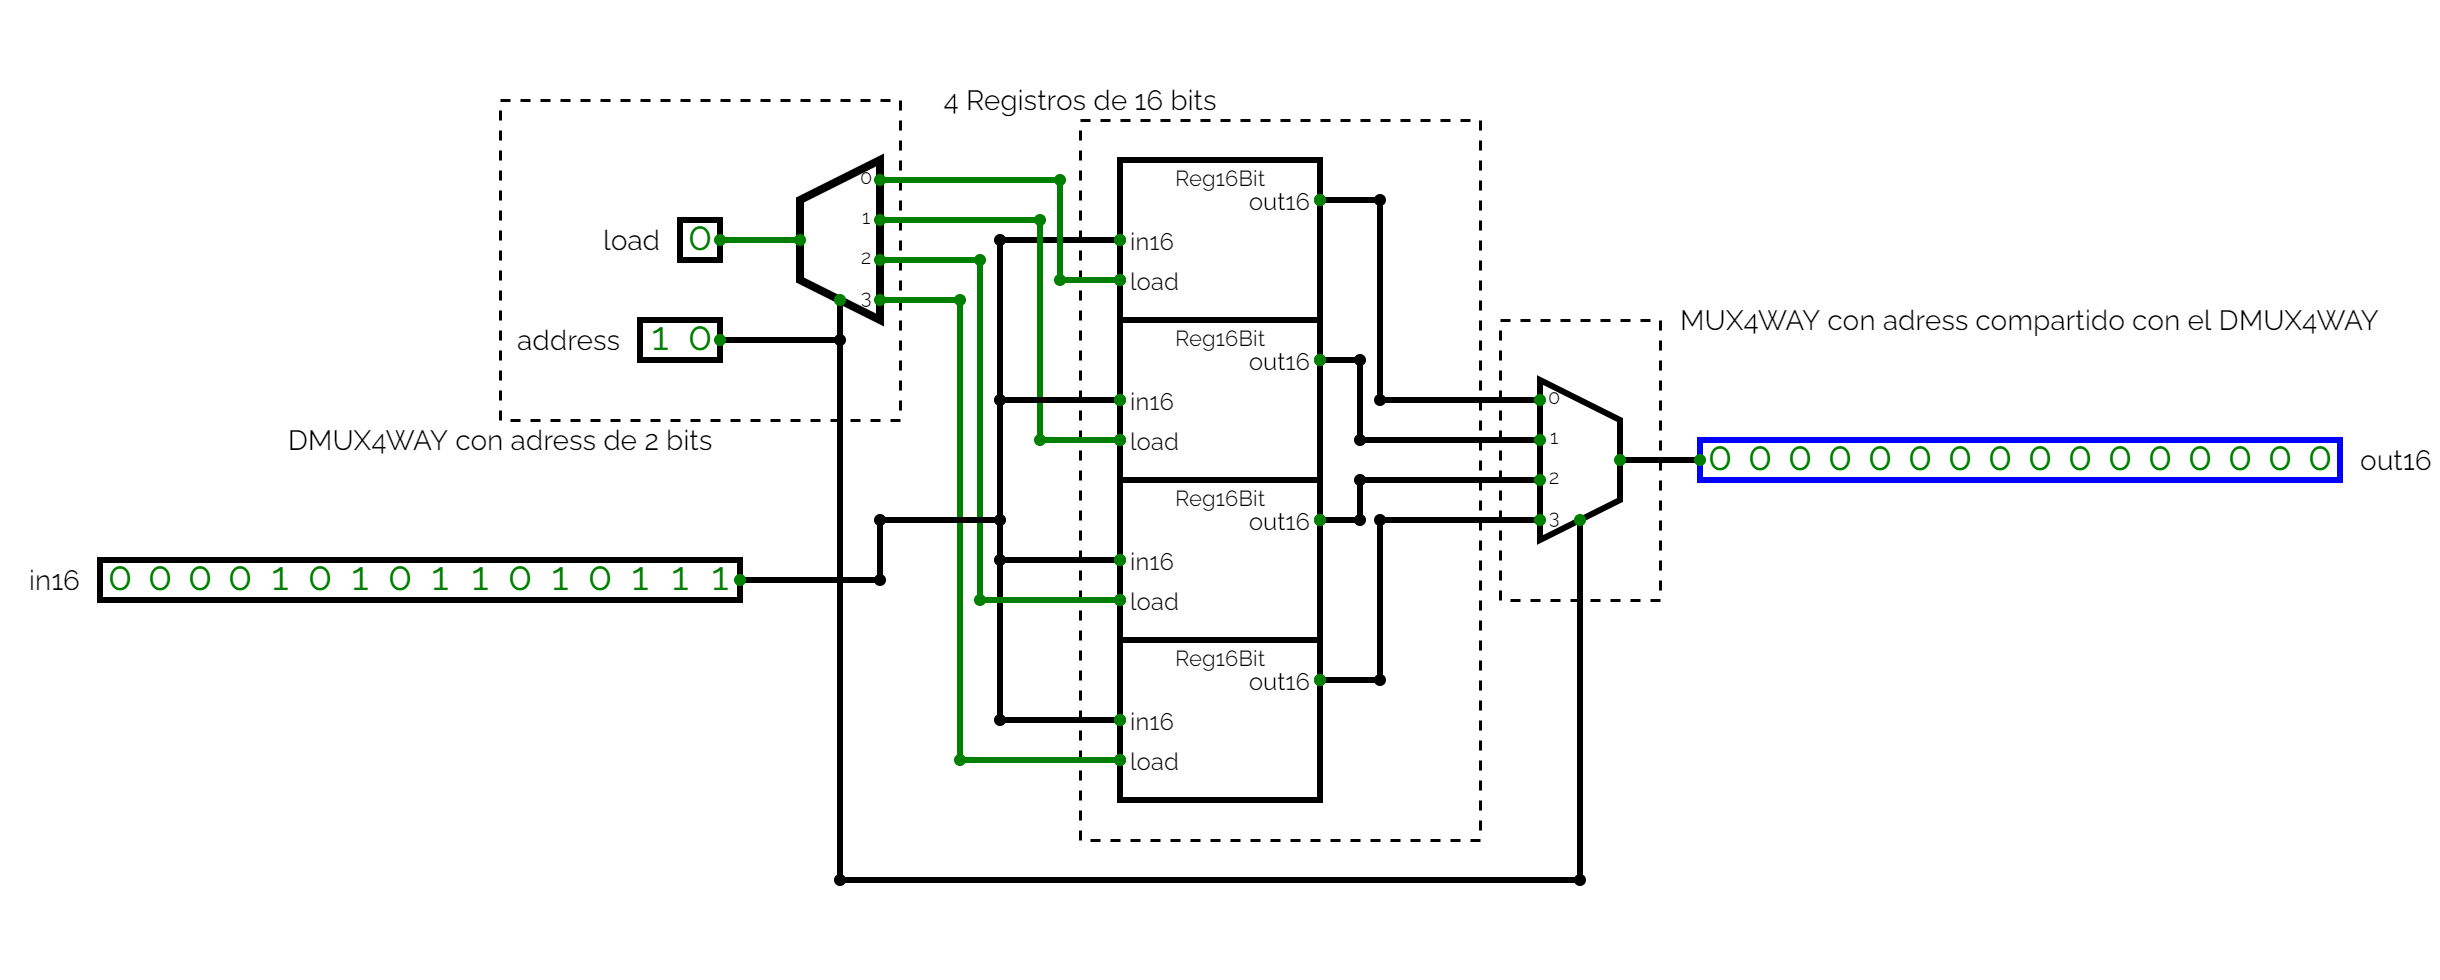
\includegraphics[width=0.75\linewidth]{RAM/RAM_int}
	\caption{Circuito interior de RAM4}
	\label{fig:ramint}
\end{figure}

Con 2 RAM4, se puede componer una RAM8.
\begin{figure}[H]
	\centering
	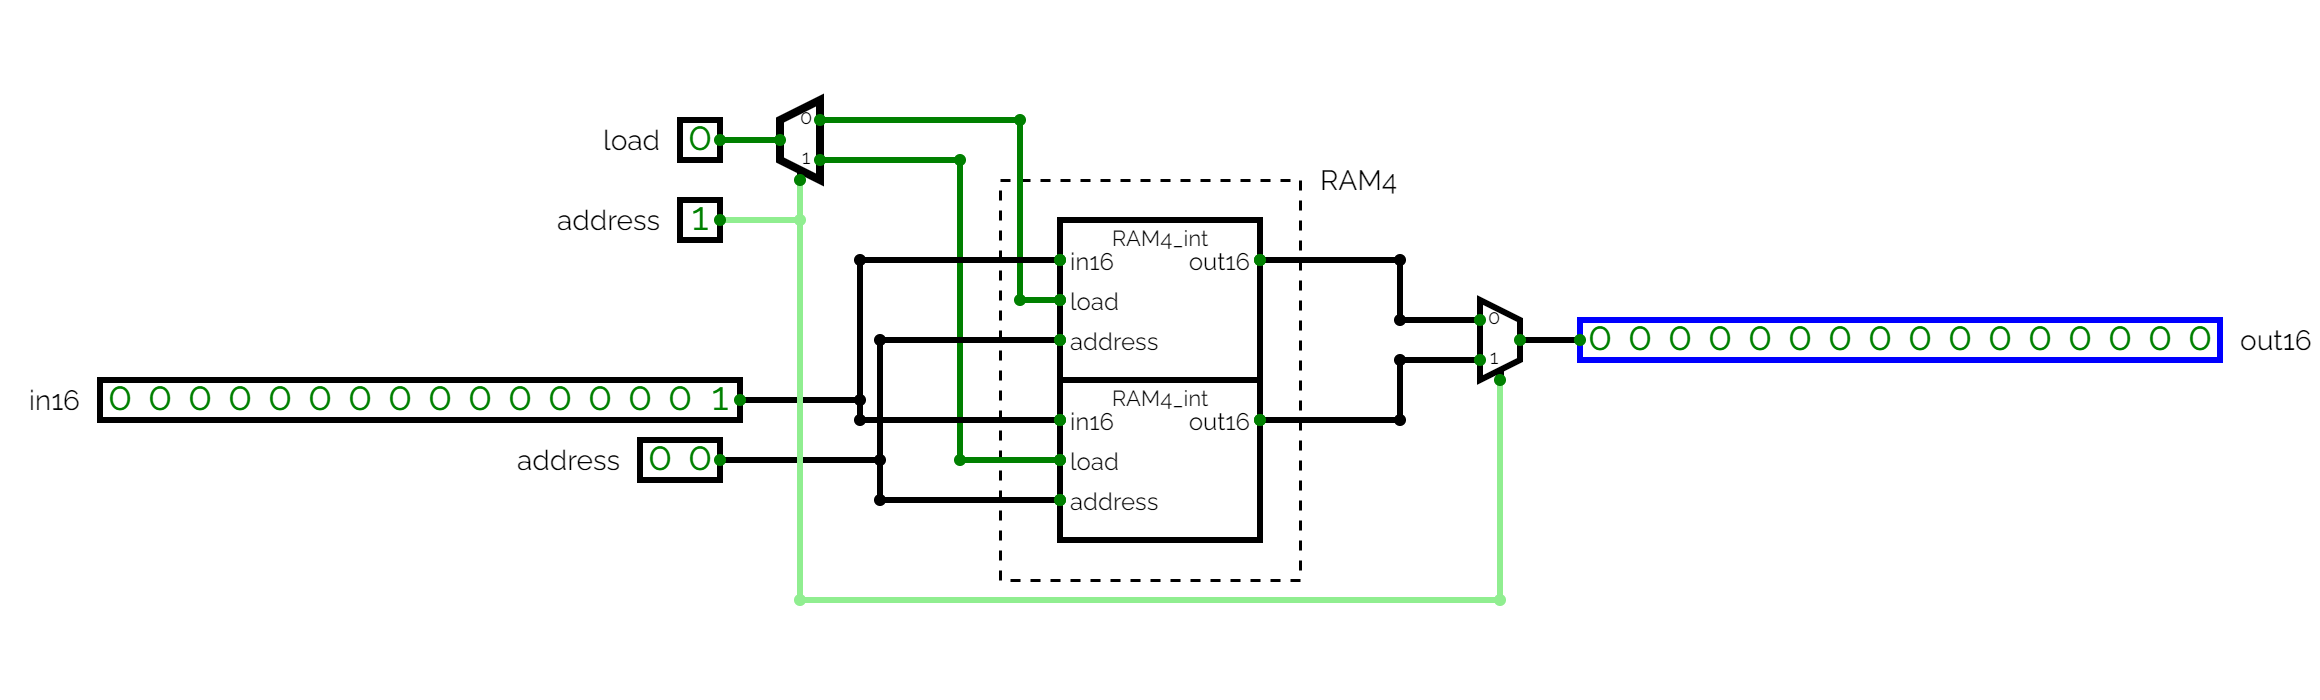
\includegraphics[width=0.75\linewidth]{RAM/RAM8_int}
	\caption{Circuito interior de RAM8}
	\label{fig:ram8int}
\end{figure}


\begin{figure}[H]
	\centering
	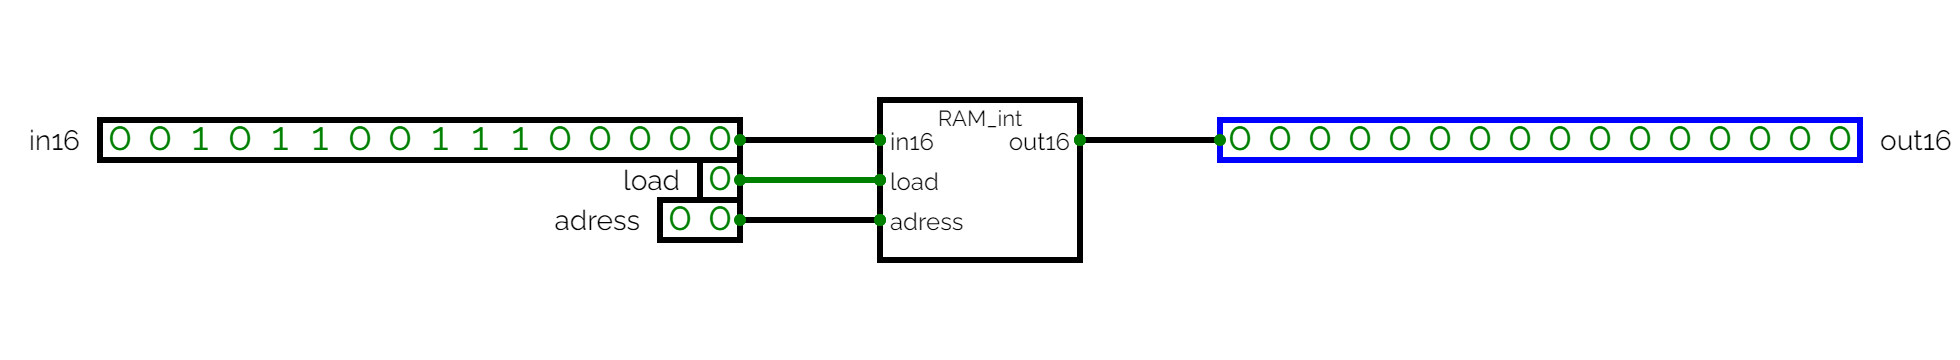
\includegraphics[width=0.75\linewidth]{RAM/RAM_EXT}
	\caption{Circuito exterior de RAM8}
	\label{fig:ramext}
\end{figure}


\subsection{Implementación HDL}
\begin{figure}[H]
	\centering
	\includegraphics[width=0.75\linewidth]{RAM/ram8_hdl}
	\caption{Implementación en Hardware Simulator de RAM8}
	\label{fig:ram8hdl}
\end{figure}

\subsubsection{Archivo .HDL}
\begin{lstlisting}
	CHIP RAM8 {
		IN in[16], load, address[3];
		OUT out[16];

		PARTS:
		DMux8Way(in=load,sel=address,a=a,b=b,c=c,d=d,e=e,f=f,g=g,h=h);

		Register(in=in,load=a,out=oa);
		Register(in=in,load=b,out=ob);
		Register(in=in,load=c,out=oc);
		Register(in=in,load=d,out=od);
		Register(in=in,load=e,out=oe);
		Register(in=in,load=f,out=of);
		Register(in=in,load=g,out=og);
		Register(in=in,load=h,out=oh);

		Mux8Way16(a=oa,b=ob,c=oc,d=od,e=oe,f=of,g=og,h=oh,sel=address,out=out);
	}
\end{lstlisting}


\newpage

%%%%%%%%%%%%%%%%%%%%%%%%%%%%%%%%%%%%%%%%%%%%%%%%%%%%%%%%%%%%%%%%%%%%%%%%%%
%%%%%%%%%%%%%%%%%%%%%%%%%%%%%%%%%%%%%%%%%%%%%%%%%%%%%%%%%%%%%%%%%%%%%%%%%%
\section{RAM64, RAM512, RAM4K y RAM 16K}
    \subsection{Explicación del circuito}
		Todas estas RAMs se comportan de una manera parecida, pero aumentando su capacidad. Todas se construyen a partir de la RAM de ocho registros \ref{ram8} y después cada una con sus anteriores, es decir, RAM64 * 8 = RAM512.

    \subsection{Esquema del circuito de la RAM64, RAM512, RAM4k y RAM16k}
		\footnotesize{\textit{NOTA: Debido a que el programa que uso para hacer los circuitos: CircuitVerse, no puede manejar la RAM64 debido a su complejidad, opto por usar un módulo prefabricado que incluye la propia página, los cuales se distinguen con un punto verde en la esquina.} }
		\begin{figure}[H]
			\centering
			\includegraphics[width=0.75\linewidth]{RAM/RAM64_int}
			\caption{Circuito de la RAM64}
			\label{fig:ram64int}
		\end{figure}

		\begin{figure}[H]
			\centering
			\includegraphics[width=0.75\linewidth]{RAM/RAM512_int}
			\caption{Circuito de la RAM512}
			\label{fig:ram512int}
		\end{figure}

		\begin{figure}[H]
			\centering
			\includegraphics[width=0.75\linewidth]{RAM/RAM4k_int}
			\caption{Circuito de la RAM4k}
			\label{fig:ram4kint}
		\end{figure}

		\begin{figure}[H]
			\centering
			\includegraphics[width=0.75\linewidth]{RAM/RAM16k_int}
			\caption{Circuito de la RAM16k}
			\label{fig:ram16kint}
		\end{figure}

    \subsection{Implementación HDL - RAM64}

        \subsubsection{Archivo .HDL}

\begin{figure}[H]
	\centering
	\includegraphics[width=0.75\linewidth]{RAM/ram64_hdl}
	\caption{Implementación HDL de RAM64}
	\label{fig:ram64hdl}
\end{figure}
        \begin{lstlisting}

CHIP RAM64 {
	IN in[16], load, address[6];
	OUT out[16];

	PARTS:

	DMux8Way(in=load,sel=address[3..5],a=a,b=b,c=c,d=d,e=e,f=f,g=g,h=h);

	RAM8(in=in,load=a,address=address[0..2],out=oa);
	RAM8(in=in,load=b,address=address[0..2],out=ob);
	RAM8(in=in,load=c,address=address[0..2],out=oc);
	RAM8(in=in,load=d,address=address[0..2],out=od);
	RAM8(in=in,load=e,address=address[0..2],out=oe);
	RAM8(in=in,load=f,address=address[0..2],out=of);
	RAM8(in=in,load=g,address=address[0..2],out=og);
	RAM8(in=in,load=h,address=address[0..2],out=oh);

	Mux8Way16(a=oa,b=ob,c=oc,d=od,e=oe,f=of,g=og,h=oh,sel=address[3..5],out=out);

}

        \end{lstlisting}

\subsection{Implementación HDL - RAM512}
  	\subsubsection{Archivo .HDL}

\begin{figure}[H]
	\centering
	\includegraphics[width=0.75\linewidth]{RAM/RAM512_hdl}
	\caption{Implementación HDL de RAM512}
	\label{fig:ram512hdl}
\end{figure}

  	\begin{lstlisting}

CHIP RAM512 {
	IN in[16], load, address[9];
	OUT out[16];

	PARTS:

	DMux8Way(in=load,sel=address[6..8],a=a,b=b,c=c,d=d,e=e,f=f,g=g,h=h);

	RAM64(in=in,load=a,address=address[0..5],out=oa);
	RAM64(in=in,load=b,address=address[0..5],out=ob);
	RAM64(in=in,load=c,address=address[0..5],out=oc);
	RAM64(in=in,load=d,address=address[0..5],out=od);
	RAM64(in=in,load=e,address=address[0..5],out=oe);
	RAM64(in=in,load=f,address=address[0..5],out=of);
	RAM64(in=in,load=g,address=address[0..5],out=og);
	RAM64(in=in,load=h,address=address[0..5],out=oh);

	Mux8Way16(a=oa,b=ob,c=oc,d=od,e=oe,f=of,g=og,h=oh,sel=address[6..8],out=out);
}

  	\end{lstlisting}

	\subsection{Implementación HDL - RAM4k}

  	\subsubsection{Archivo .HDL}
	\begin{figure}[H]
		\centering
		\includegraphics[width=0.75\linewidth]{RAM/RAM4k_hdl}
		\caption{Implementación HDL de RAM4k}
		\label{fig:ram4khdl}
	\end{figure}
  	\begin{lstlisting}

CHIP RAM4K {
	IN in[16], load, address[12];
	OUT out[16];

	PARTS:
	DMux8Way(in=load,sel=address[9..11],a=a,b=b,c=c,d=d,e=e,f=f,g=g,h=h);

	RAM512(in=in,load=a,address=address[0..8],out=oa);
	RAM512(in=in,load=b,address=address[0..8],out=ob);
	RAM512(in=in,load=c,address=address[0..8],out=oc);
	RAM512(in=in,load=d,address=address[0..8],out=od);
	RAM512(in=in,load=e,address=address[0..8],out=oe);
	RAM512(in=in,load=f,address=address[0..8],out=of);
	RAM512(in=in,load=g,address=address[0..8],out=og);
	RAM512(in=in,load=h,address=address[0..8],out=oh);

	Mux8Way16(a=oa,b=ob,c=oc,d=od,e=oe,f=of,g=og,h=oh,sel=address[9..11],out=out);
}

  	\end{lstlisting}

  	    \subsection{Implementación HDL - RAM16k}

  	\subsubsection{Archivo .HDL}

\begin{figure}[H]
	\centering
	\includegraphics[width=0.75\linewidth]{RAM/RAM16k_hdl}
	\caption{Implementación HDL de RAM16k}
	\label{fig:ram16khdl}
\end{figure}
  	\begin{lstlisting}

CHIP RAM16K {
	IN in[16], load, address[14];
	OUT out[16];

	PARTS:
	DMux4Way(in=load,sel=address[12..13],a=a,b=b,c=c,d=d);

	RAM4K(in=in,load=a,address=address[0..11],out=oa);
	RAM4K(in=in,load=b,address=address[0..11],out=ob);
	RAM4K(in=in,load=c,address=address[0..11],out=oc);
	RAM4K(in=in,load=d,address=address[0..11],out=od);

	Mux4Way16(a=oa,b=ob,c=oc,d=od,sel=address[12..13],out=out);
}

  	\end{lstlisting}

\newpage
%%%%%%%%%%%%%%%%%%%%%%%%%%%%%%%%%%%%%%%%%%%%%%%%%%%%%%%%%%%%%%%%%%%%%%%%%%
%%%%%%%%%%%%%%%%%%%%%%%%%%%%%%%%%%%%%%%%%%%%%%%%%%%%%%%%%%%%%%%%%%%%%%%%%%
\printbibliography[heading=bibintoc]
\end{document}
